\documentclass[a4paper,12pt]{book}
\usepackage[italian]{babel}
\usepackage[T1]{fontenc}
\usepackage[utf8]{inputenc}
\usepackage{todonotes}
\usepackage{caption}
\usepackage{subfig}
\usepackage[version=3]{mhchem}
\usepackage{textcomp}
\usepackage{float}
%\DeclareGraphicsExtensions{.jpg}
\captionsetup{format=hang,labelfont={sf,bf}}
\usepackage{amsmath,amssymb}
\usepackage{xspace}
\usepackage[hidelinks]{hyperref}
\usepackage{chemfig}
\usepackage{mhchem}

\newcommand{\freccia}{\ensuremath{\rightarrow}}
\newcommand{\lfreccia}{\ensuremath{\longrightarrow}}


\begin{document}
\author{Elisa Nerli}
\title{Fisiologia vegetale}
\maketitle
\newpage
\tableofcontents
\newpage




\chapter{Relazioni Idriche}
L'ambiente acquoso è importante per le piante per la struttura molecolare e per la struttura cellulare.

Il passaggio dalla vita acquatica alla vita terrestre comporta:
\begin{itemize}
   \item{Apparato radicale: per captazione dell'acqua} 
    \item{Rivestimento di cutina: 
    \begin{enumerate} 
    \item{Evitare perdita di acqua + apertura degli stomi.}
    \item{Collegato alla \emph{traspirazione}, movimento di acqua attraverso la pianta}
    \end{enumerate}}
\end{itemize}
Ovviamente è necessario un sistema di regolazione di questi fenomeni.

Turgore: acqua che esercita pressione idrostatica contro la parete. Essenziale per il corretto svolgimento delle funzioni delle piante, e per mantenerle erette.


L'acqua è il solvente universale:
\begin{itemize}
    \item{impedisce l'aggragazione tra le molecole cariche;}
    \item{mantiene integrità strutturale della cellula;}
    \item{mantiene la temperatura della pianta costante.}
\end{itemize}

I nutrienti vengono traslocati nella pianta grazie al flusso d'acqua (transiente, ovvero l'acqua è sempre in movimento):
\begin{itemize}
\item{Discendente}
\item{Ascendente}
\end{itemize}

Servono comunque grandi quantità di acqua per far crescere una pianta: 250 L a stagione per pianta di mais.
L'accrescimento è quindi lento in confronto alla disponibilità di acqua (questo varia in base al metabolismo delle cellule).
Il contenuto idrico varia anche nelle stesse cellule (nel vacuolo, 90-95\%): negli organi in accrescimento varia tra l'80\% e il 90\% della massa totale.
 
\paragraph{Contenuto idrico}
Per valutare il contenuto idrico:
\begin{enumerate}
\item{Pesare una fronda per determinare il peso fresco (FW)}
\item{Metterla in stufa a 103 \textcelsius}
\item{Raffreddare il tessuto in un essiccatore contenente silice granulata}
\item{Pesare di nuovo il tessuto per misurarne il peso secco (DW)} 
\end{enumerate}
A questo punto si procede con il calcolo del contenuto idrico:
\begin{equation*}
\centering
	\% H_{2}O=\frac{(FW-DW) \cdot 100}{FW}
\end{equation*}

\section{Caratteristiche molecolari dell'acqua}

\chemfig{H-[:52.24]\lewis{1:3:,O}-[::-104.48]H}

Molecola d’acqua con i due atomi di idrogeno legati covalentemente all’atomo di ossigeno. Le cariche parziali opposte fra molecole di acqua vicine tendono ad attrarsi originando una debole interazione elettrostatica nota come legame ad idrogeno.

Le molecole di acqua possono formare interazioni elettrostatiche con ioni e legami ad idrogeno
con sostanze organiche (urea nell’esempio) che contengono atomi elettronegativi (O oppure
N).\todo{Ripassa: struttura molecola; interazioni elettrostatiche; legame a H}

\paragraph{Proprietà di termoregolazione}

\begin{itemize}
\item{Alto calore specifico}
\item{Alto calore latente di evaporazione\footnote{energia di calore necessaria per spostare a temperatura costante molecole di acqua dallo stato liquido alla fase gassosa} (abbassamento T pianta) insieme a traspirazione}
\end{itemize}

\paragraph{Proprietà di coesione e adesione}

\begin{itemize}
\item{Le molecole di acqua che restano vicine creano una forza intensa, che genera una \emph{tensione superficiale}\footnote{Energia necessaria ad aumentare l'area di un'interfaccia liquido-gas.}}
\item{L'attrazione tra molecole d'acqua e superfici solide determina l'\emph{adesione}}
\end{itemize}

L'adesione verso superfici idrofile si può vedere immergendo un tubicino idrofilico in acqua: si forma una concavità e si ha risalita dell'acqua (menisco concavo). Se immergo un tubicino idrofobico, non si ha risalita dell'acqua e si ha solo tensione superficiale, non adesione.

\section{Come avviene il movimento d'acqua?}
Il movimento d'acqua può avvenire per:
\begin{enumerate}
\item{Diffusione: gradiente di concentrazione}
\item{Flusso di massa: gradiente di pressione}
\item{Osmosi: gradiente di potenziale idrico}
\end{enumerate}

\subsection{Diffusione}
Spostamento di acqua a breve distanza da regioni ad alta concentrazione a regioni a bassa  concentrazione. Moto browniano indirizzato verso i plasmodesmi.

Il movimento per diffusione è descritto dalla \textbf{Legge di Fick}:
\begin{equation}
J_{H_{2}O}=- \frac{D_{H_{2}O} \Delta C_{H_{2}O}}{L}
\centering
\end{equation}

dove J è la densità di flusso, D è il coefficiente di diffusione, $\Delta C$ è la differenza di concentrazione ed L è la distanza.
Il segno - indica che il flusso va da una zona ad alta concentrazione ad una a più bassa concentrazione.

Da questa legge possiamo ricavare anche un'altra relazione, che determina il tempo necessario ad una sostanza s per raggiungere un punto situato ad una distanza d dal punto di partenza, tale che la concentrazione sia la metà di quella iniziale:
\begin{equation}
t_{c=0,5}=\frac{d^2}{D_{s}} \cdot K
\centering
\end{equation}

dove K=1.

La diffusione è un fenomeno adatto solo al trasporto a breve distanza.  

(1.10.2014)
\subsection{Flusso di massa}
In fisiologia vegetale interessa soprattutto il flusso di massa dell’acqua e dei soluti in essa
disciolti in condotti di piccolo diametro come i pori del suolo, i vasi xilematici e i tubi floematici.
Esso è descritto dall’equazione di Hagen-Poiseuille:
\begin{equation}
\centering
J_{H_{2}O}= - \frac{\pi r^{4}}{8 \eta} \cdot \frac{\Delta \Psi_{H_{2}O}}{L}
\end{equation}
in cui r è il raggio del capillare e $\eta$ la \emph{viscosità} del liquido, mentre $\frac{\Delta \Psi_{H_{2}O}}{L}$ è il \emph{gradiente di pressione} nel capillare.

Il flusso di massa è ideale per il trasporto a lunga distanza perchè è molto più veloce della diffusione: per il movimento dell'acqua nei vasi xilematici e floematici, ma anche a livello del suolo e dal suolo alla pianta (all'apparato radicale della pianta, per essere precisi), a livello dell'apoplasto, spazio intercellulare costituito dalla parete cellulare di cellule adiacenti. 

\subsection{Osmosi}
Movimento di acqua attraverso una membrana semipermeabile, che somma diffusione e flusso di massa. Il movimento di acqua continua per diffusione fino a che le concentrazioni non sono uguali.

Interviene anche un fenomeno legato alla pressione per cui il movimento può essere legato alla pressione: applicando una pressione su una delle due metà della vasca, il movimento dell'acqua rallenta e viene impedito \lfreccia gradiente di pressione.
Nelle cellule vegetali il processo comporta entrambe i tipi di movimento.

C'è anche un movimento dovuto alla forza motrice che è il gradiente di potenziale idrico. Ci sono canali attraverso i quali l'acqua entra nella cellula secondo il fenomeno di flusso di massa, mentre la diffusione di poche molecole di acqua avviene nel doppio strato.

L'acqua poi entra all'interno delle cellule e si muove nel \emph{simplasto}, spostandosi da una cellula all'altra per diffusione.

\section{Potenziale idrico}
Lo spostamento richede un imput energetico: l'acqua si sposta da un contenuto energetico X ad un contenuto energetico < X.
Il \emph{potenziale chimico} $\mu_{w}$ esprime l’energia libera associata ad una sostanza (nel nostro caso l'acqua). Va
ricordato che l’energia libera rappresenta il potenziale a compiere un lavoro. Processi come le reazioni biochimiche, l’accumulo di soluti ed il trasporto a lunga distanza, sono resi possibili da un apporto di energia libera.

\begin{equation}
\centering
\mu_{w}=RT ln \ {} a_{w} + PV_{w} + ghm_{w}
\end{equation}
dove $m_{w}$ è la massa dell'acqua.

Definiamo il potenziale idrico $\Psi_{w}$ come il lavoro necessario per spostare 1 molecola di $H_{2}O$ pura, da un comparto contenente $H_{2}O$ pura ad un comparto contenente una soluzione diluita.
Il potenziale idrico di una pianta viene espresso come il lavoro necessario per portare l'acqua
legata biologicamente al livello di potenziale di acqua pura. È espresso in \emph{unità di pressione}, anzichè in unità di energia.

È definito come il potenziale chimico dell'acqua diviso il volume parziale molare dell'acqua.

Dividendo l'equazione del potenziale chimico per il volume parziale molare dell'acqua, otteniamo:
\begin{equation}
\centering
\Psi_{w}= \frac{\mu_{w}}{V_{w}}= \frac{RT ln \ {} a}{V} + \frac{PV}{V} + \frac{mgh}{V}
\end{equation}

dove $\frac{RT ln \ {} a}{V}$ è la componente osmotica $\Psi_{s}$, $\frac{PV}{V}$ è la componente idrostatica $\Psi_{p}$ e $\frac{mgh}{V}$ la componente gravitazionale $\Psi_{g}$.

Il termine $\Psi_{s}$ è chiamato il \emph{potenziale di soluto}\footnote{o potenziale osmotico} e rappresenta l'effetto dei soluti disciolti sul potenziale idrico. I soluti riducono l'energia libera dell'acqua diluendola.

Il termine $\Psi_{p}$ indica il \emph{potenziale di pressione} della soluzione. Pressioni positive incrementano il potenziale idrico, negative lo riducono.

Il termine $\Psi_{g}$ indica il \emph{potenziale gravitazionale}. Si può indicare la massa dell'acqua come $\rho_{w} V$, che ha un valore di 0,01 MPa $m^{-1}$. Di solito si omette nelle considerazioni riguardo il trasporto dell'acqua a livello cellulare. Dipende dalla densità dell’acqua, dalla gravità e dall’altezza. Di solito aumenta di 0,01 MPa per metro di altezza.

Esiste poi il termine $\Psi_{m}$, detto \emph{potenziale di matrice}, che esprime l'influenza dell'interfaccia liquido-solido, ma il cui effetto è già rappresentato da $\Psi_{s}$ e da $\Psi_{p}$. Assume valori negativi perché le molecole di acqua, all'interfaccia con un solido,
hanno minore tendenza a reagire chimicamente, evaporare, etc. (cioè hanno
minore energia libera).
E' importante nei suoli asciutti, nei tessuti disidratati (semi) e nelle pareti cellulari
scarsamente idratate.

Se h<5-10 m, trascuriamo la gravità, e se le componenti di una pianta sono idratate, trascuriamo $\Psi_{m}$. Riduciamo quindi l'espressione del potenziale idrico a:
\begin{equation}
\centering
\Psi_{w}= \Psi_{s} + \Psi_{p}
\end{equation}

Per piante non adatte a vivere in ambienti salini, in condizione di bassa idratazione, è molto difficile assumere acqua dall'esterno. 

\subsection{Diagramma di Hofler}
Modo per schematizzare le variazioni del potenziale idrico a seconda delle variazioni del potenziale di soluto. Mostra infatti le relazioni esistenti tra potenziale osmotico, potenziale idrico, potenziale di turgore e volume cellulare.
\begin{figure}[H]
\centering
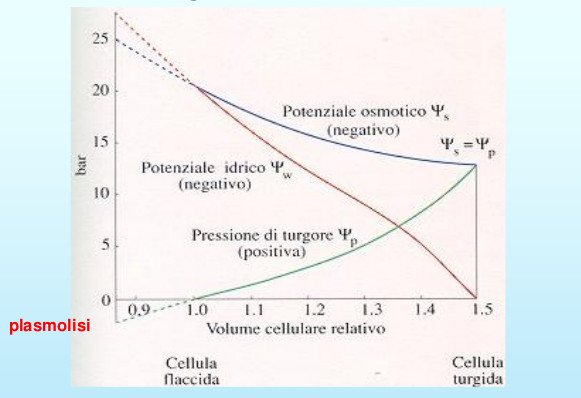
\includegraphics[scale=0.4]{immagini/hofler.jpg}
\caption{Diagramma di Hofler}
\end{figure}

Si parte da una cellula vegetale flaccida, ovvero idratata ma non al punto tale da comprimere il vacuolo. 
\begin{itemize}
\item{Se cellula flaccida volume cellulare relativo 1, allora potenziale idrico = potenziale osmotico}
\item{Se l'acqua inizia ad entrare per osmosi, il protoplasto aumenta di volume, fino ad occupare tutto il volume a disposizione (fino a che la pressione di turgore = pressione esercitata dalla parete sul vacuolo). Si ha diminuzione di Cs, quindi del potenziale osmotico. Aumenta il potenziale di turgore  e il potenziale idrico diminuisce man a mano che entra acqua nella cellula. Allora potenziale di soluto = potenziale di pressione, e quello idrico sarà = 0

Quando la cellula sarà al massimo turgore, l'acqua non entrerà più.}
\item{Se l'acqua esce : cellula plasmolisata. Il protoplasto si contrae fino a rottura, perdita di adesione del protoplasto alla parete cellulare}
\end{itemize}

La \emph{parete cellulare} consente alla cellula vegetale di adattarsi alle condizioni presenti. La parete consente di interrompere l'assunzione di acqua.

(6.10.2014)

\paragraph{Plasmolisi}
 I cordoni citoplasmatici sono delle strutture composte di fibrille, microfibrille di cellulosa, filamenti di actina attorno ai quali si distribuisce la membrana plasmatica a seguito della contrazione del protoplasto, in modo tale che resti distesa.
Non sempre la plasmolisi può avere un decorso favorevole: solo entro lo stadio di plasmolisi incipiente questa è reversibile. A quel punto, la cellula può di nuovo plasmolisare.

\section{Metodi per la misurazione del potenziale idrico dei tessuti}

\begin{enumerate}
\item{Immersione di frammenti di tessuto in soluzioni a diverse concentrazioni, via via crescenti, fino a che non troviamo la soluzione isotonica con il tessuto immerso. Si utilizzano sali o molecole organiche non metabolizzate (es. manitolo, saccarosio - questo assunto in minima parte).
Si valuta se il peso del tessuto è cambiato. La soluzione isotonica ha una concentrazione che ci permette di calcolare il potenziale idrico}

\item{Bomba a pressione: apparecchiatura collegata ad erogatore di aria compressa. Recidere un ramo della pianta e misurare la pressione che serve a controbilanciare la tensione esistente all'interno dei tessuti (all'interno dei vasi xilematici, esiste una tensione, o pressione negativa: recidendo un ramo, l'acqua recede dalla superficie di taglio \lfreccia menisco ricurvo).
Il ramo è inserito nell'apparecchiatura, nella quale si esercita pressione rilasciandovi aria compressa: con il manometro misuriamo la pressione che serve a far rialzare il menisco nel ramo tagliato.
Facendo un grafico della variazione del peso nel tempo, si ottiene una curva che  cresce fino al \emph{plateau}, la pressione che equivale alla pressione idrostatica all'interno dello xilema. Assumiamo il potenziale osmotico trascurabile, poichè non sto assorbendo nè perdendo acqua. il potenziale idrico sarà quindi l'opposto della pressione idrostatica}
\end{enumerate}


\chapter{Movimento dell'acqua: suolo, pianta e atmosfera}

L'acqua non presenta una soluzione di continuità dal suolo all'atmosfera: segue però un percorso che dal suolo la porta all'atmosfera passando per la pianta, detto \emph{continuum suolo-pianta-atmosfera}:

suolo \lfreccia peli radicali \lfreccia cilindro vascolare (xilema) \lfreccia spazi intercellulari al livello del meristema, parenchima fotosintetico \lfreccia evaporazione per traspirazione.

\section{Il suolo}
Il suolo è una miscela di materiali, alcuni in forma solida (particelle minerali), più o meno in soluzione.
\begin{itemize}
\item{45\% : componente minerale}
\item{50\% : aria ed acqua, che circolano nei pori tra le particelle del suolo}
\item{5\%  : componente organica, composta da Humus (80\%), radici (10\%) e microfauna e flora (10\%)}
\end{itemize}
Il profilo del suolo è composto da una serie di strati, gli \emph{orizzonti}:
\begin{itemize}
\item{Orizzonte O: organico, humus + lettiera vegetale. Strato inerte dal punto di vista di nutrimento delle piante}
\item{Orizzonte A: il materiale organico inizia ad essere degradato e a costituire nutrimento, permettendo al suolo di trattenere ioni ed acqua. Le sostanze più fini, tipo l'argilla, vengono dilavate da questo strato, scendendo verso il basso, e si portano dietro le componenti colloidali che vanno nello strato illuviale}
\item{Orizzonte B: strato illuviale, dilavamento dell'argilla, assenza di pigmenti}
\item{Orizzonte C: roccia che dà origine ai materiali minerali, iniziale trasformazione della roccia madre, ma non presenta modificazione da parte di sostanze organiche \lfreccia no nutrimento piante}
\item{Orizzonte R: roccia madre, non trasformata}
\end{itemize}

Le particelle più grandi che troviamo nel suolo sono quelle di \emph{sabbia}, di forma irregolare. Sono inerti e conferiscono al suolo una porosità elevata: ciò provoca grande circolazione di acqua ed aria (non troppo positivo).

Le particelle di \emph{limo} hanno dimensioni un poco inferiori: superficie liscia appiattita \lfreccia suolo compatto, che trattiene acqua, la quale circola male.

Le particelle di \emph{argilla }sono le più piccole, fromate da silicati di alluminio, che costituiscono un reticolo cristallino caratterizzato da carica superficiale netta negativa (trattenimento di cationi).
L'argilla costituisce cristalli con grande capacità di solvatazione \lfreccia le cariche - interagiscono con i dipoli dell'acqua, quindi l'argilla riesce a trattenere discrete quantità di acqua. Gli spazi tra le particelle sono piuttosto piccoli (micropori).

Certi cationi vengono legati meglio di altri: i bivalenti sono legati più fortemente. Es. magnesio lega meglio del calcio: importante perchè le piante hanno bisogno di determinate dosi dei vari elementi. 

\emph{Qual è il suolo ideale per la crescita delle piante?}

Dobbiamo guardare la \emph{tessitura del suolo}: in laboratorio, mediante setacciatura del suolo essiccato. Si risale al tipo di terreno grazie al \emph{triangolo tessiturale}: si hanno terreni di sabbia, argilla e limo. Vediamo che quello che favorisce meglio lo sviluppo delle piante è la parte in blu, LOAM, in cui nessuna frazione (sabbia, argilla o limo) prevale sulle altre.

Le caratteristiche che influenzano la tessitura e le proprietà del suolo sono:
\begin{itemize}
\item{Areazione}
\item{Drenaggio}
\item{Capacità di trattenere nutrienti}
\item{Capacità di trattenere acqua}
\end{itemize}

Un suolo sabbioso ha un'eccellente areazione e drenaggio, ma bassa capacità di trattenere nutrienti ed acqua.

Un suolo limoso ha buone areazione e drenaggio e media capacità di trattenere nutrienti ed acqua.

Un suolo argilloso ha bassa capacità di drenaggio ed areazione, ma alta capacità di trattenere nutrienti, che lega, ed acqua.
\subsection{Struttura}
La struttura del terreno è importante: un terreno meno compatto favorisce la circolazione di acqua ed aria. Il terreno può avere struttura:
\begin{enumerate}
\item{A particelle singole: non si aggregano fra loro}
\item{A particelle aggregate: si aggregano (humus)}
\end{enumerate}

Le singole particelle del suolo tendono ad aggregarsi per attrazione fisica e chimica. Cationi come il calcio , il magnesio e l’alluminio con più di una carica positiva agiscono come un \emph{ponte elettrostatico} che lega insieme due particelle di argilla cariche negativamente. Terreni con struttura ottimale hanno ampi spazi vuoti che aumentano il movimento dell’aria e dell’acqua nel suolo.
A seconda della quantità di materia organica, si hanno diverse compattezze: meno ce n'è, meno è compatto il suolo.

\paragraph{Humus} si trova nel livello che comprende l'apparato radicale, sopra la componente argillosa. È ciò che deriva dalla decomposizione della sostanza organica dai microrganismi del suolo. Può essere labile o stabile:
\begin{itemize}
\item{Labile: dato da macromolecole, primi prodotti della decomposizione della materia orgnaica}
\item{Stabile: molecole che hanno subito un ulteriore processo di degradazione. Gli elementi che lo compongono sono : C, N, P (di fosforo solo lo 0.5\%, di carbonio il 50\%)}
\end{itemize}

\paragraph{}
L'acqua nel suolo è presente in modo variabile: le variazioni sono date dalla presenza delle piante, che assorbono continuamente acqua dal suolo, e anche dall'evaporazione dell'acqua dalla superficie del suolo e dalla risalita dell'acqua nel suolo per capillarità. Il richiamo dell'acqua dagli strati più profondi è favorito dalla pianta.

La capacità che un suolo ha di trattenere acqua è detta \emph{capacità di campo}, ovvero la quantità di acqua per grammo del suolo. Si pesa un campione di suolo, si satura di acqua, si lascia sgocciolare per togliere l'acqua in eccesso e si ripesa il campione, misurando così la quantità di acqua trattenuta. 

Nel suolo sono presenti \emph{pori}, nei quali si trova aria circolante. A seguito dei processi di adesione e coesione, si ha una maggior disponibilità di acqua nelle parti più prossime alla superficie, e via via che ci si allontana il quantitativo di acqua si assottiglia fino all'arrivo alla superficie del poro. L'acqua tende quindi ad aderire alle particelle solide, creando interstizi nei quali l'aria può circolare.

L'acqua può penetrare all'interno della radice grazie ad una \emph{differenza di potenziale idrico}, negativo per la pianta e meno negativo per il suolo. Questo \emph{potenziale idrico del suolo} ha le 3 componenti del potenziale idrico. 
 
\textbf{Come si genera questo potenziale nel suolo?}

Sempre grazie a processi che sviluppano la tensione superficiale a livello di spazi in cui l'acqua è a contatto con l'aria (forze di adesione e coesione generano questa tensione superficiale). Man a mano che l'acqua viene richiamata dalle piante, diminuisce la superficie e si creano zone con menischi ricurvi. La formazione di essi si traduce nella generazione di una tensione nell'acqua a livello del suolo: si forma come si forma nel mesofillo fogliare.

\begin{equation}
\centering
\Psi_{P}=- \frac{2T}{r}
\end{equation}
dove T è la tensione superficiale ed r il raggio di curvatura dell'interfaccia aria-acqua.


Il potenziale idrico molto negativo si forma perchè quello osmotico è sempre negativo (-0.002 MPa) e spesso trascurabile, la componente data dalla pressione è negativa o 0 a seconda dello stato di solvatazione del suolo. 
Più il suolo diventa arido, più influisce il potenziale osmotico, che dipende direttamente dalla concentrazione dei soluti. Nei suoli secchi infatti il raggio di curvatura dell'interfaccia aria-acqua è molto più piccolo.
Nei suoli salini, l'effetto è ancora più elevato. Nei suoli umidi, $\Psi_{P}$ è circa 0.

Aumentare il potenziale osmotico fa si che all'interno della pianta, affinchè si possa richiamare acqua, debba svilupparsi un potenziale idrico ancora più negativo. Le piante che riescono a farlo, sono adattate a queste circostanze grazie al fatto che nei vacuoli delle cellule radicali ci sono altissime concentrazioni di sali. Solo così riescono a richiamare acqua.

\subsection{pH del suolo}
Determinato con pHmetri o con cartine indicatrici.
Vi sono piante acidofile (azalee, rododendri, ortensie) e piante alcaline (rose).

Il pH è legato alla capacità del suolo di rendere o meno disponibili determinati elementi necessari alla crescita delle piante. La maggior parte di questi elementi sono maggiormente disponibili a pH leggermente acidi (disponibilità legata al pH del  suolo).

\paragraph{Scambio cationico dell'argilla} l'argilla lega cationi (con capacità diverse). A seconda delle concentrazioni relative dei cationi, essi saranno diversamente disponibili per la pianta.


\section{Assorbimento di acqua a livello della radice}
In prossimità della radice c'è  una \emph{zona di esaurimento} dei nutrienti, che vengono assorbiti dai peli radicali. La zona di ingerenza della radice si amplia nel suolo proprio grazie a questi peli : es. il segale ha 625 km/pianta di radici, comprende una superficie di 230 $m^{2}$.


I peli si trovano nella parte alta della radice: qui aumentano l'assorbimento penetrando negli spazi tra le particelle del suolo. Nella parte del root cap e del centro quiescente invece l'acqua entra in modo più lento, guidata dall'osmosi. L'acqua entra per diffusione, richiamata dai soluti disciolti all'interno delle cellule (scarsa). 
\begin{figure}[H]
\centering
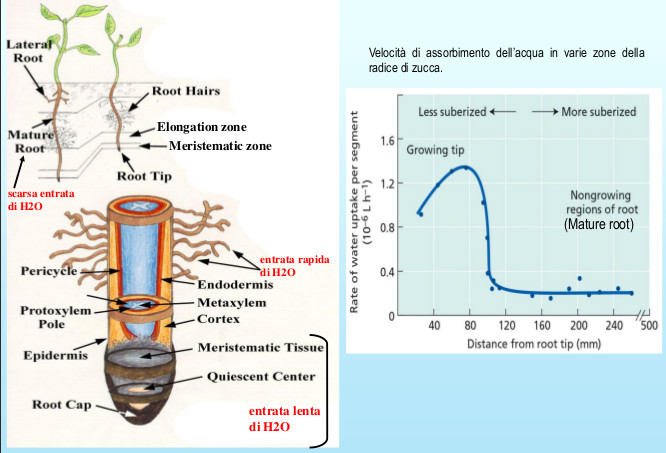
\includegraphics[scale=0.5]{immagini/radice.jpg}
\caption{Distribuzione dei peli radicali e velocità di assorbimento}
\end{figure}
Nei peli radicali, l'acqua entra per omosi: le cellule hanno grandi e numerosi vacuoli. Nel cilindro centrale è presente una tensione: genera un potenziale idrico più basso nello xilema rspetto alle cellule del pelo radicale, e quindi l'acqua si sposterà dei peli radicali verso lo xilema. 
I peli radicali sono fragili, vengono danneggiati rapidamente (vita media 2 gg).

Se vediamo il grafico di assorbimento di acqua nelle varie zone della radice, a partire dall'apice radicale si ha assorbimento che aumenta avvicinandosi alla zona che presenta peli radicali. Man a mano che ci allontaniamo, diminuisce drasticamente perchè si ha suberizzazione della parete delle cellule.

\paragraph{Xilema} trasporto linfa ascendente.
L'acqua può compiere due percorsi, attraverso:
\begin{enumerate}
\item{Cellule dei peli radicali}
\item{Cellule della corteccia}
\item{Endodermide (strisce del caspari, zone di impermeabilizzazione)}
\item{Periciclo}
\item{Cilindro centrale}
\item{Floema}
\end{enumerate}

Le vie che l'acqua può percorrere, nella parte iniziale, sono:
\begin{itemize}
\item{Via simplastica: \emph{attraversa i citoplasmi} delle cellule dei parenchimi, fino a che non raggiunge l'endodermide e poi lo xilema}
\item{Via apoplastica: l'acqua scivola esternamente alla membrana plasmatica, muovendosi \emph{all'interno delle pareti}, ma non entrando nella cellula. Questo richiede meno resistenze rispetto alla via simplastica. L'acqua raggiunge sempre l'endodermide, ma si ferma, non arriva allo xilema perchè le cellule dell'endodermide, a causa della presenza della banda del Caspari, sono impermeabilizzate: l'acqua deve  quindi per forza entrare all'interno delle cellule per arrivare allo xilema}
\end{itemize} 
La radice è un organo che non solo si relaziona al suolo per captarne elementi, ma essa stessa modifica il suolo nella rizosfera. Questa modificazione deriva da azioni legate ai rapporti stabiliti con alcuni microrganismi del suolo (simbiosi micorrizziche con gli attinomiceti, oppure simbiosi con batteri azotofissatori). Le piante emettono sostanze che favoriscono l'istaurarsi di simbiosi, la produzione di mucillaggini, l'acquisizione di nutrienti, l'assorbimento di ferro con sostanze chelanti; anche l'alterazione del pH nella zona prossima alla radice è importante \lfreccia terreno più acidificato intorno alla matrice che favorisce il trasporto attivo di ioni: l'apoplasto, nel quale vengono rilasciati i protoni nella radice, è in equilibrio con le particelle del suolo grazie all'acqua.

\subsection{Salita della linfa grezza}
Nella maggior parte delle piante, lo xilema costituisce la parte più lunga della rete di trasporto dell'acqua. Ha bassa resistenza

Lo xilema è formato da due tipi di vasi: \emph{tracheidi} e gli \emph{elementi dei vasi}. Le tracheidi si trovano in angiosperme e gimnosperme, gli elementi dei vasi solo nelle angiosperme e in un piccolo gruppo di gimnosperme. La maturazione di questi vasi coinvolge la deposizione della parete secondaria e la morte delle cellule.\todo{ricontrolla su botanica}
 
Nei vasi si ha frequentemente occlusione: si occludono zone più o meno ampie di una trachea o di una tracheide. Le perforazioni laterali permettono di isolare questo vaso e di far andare l'acqua nel vaso accanto, in modo tale che il flusso di acqua non si blocchi.

(8.10.2014)


Attraverso lo xilema, l'acqua attraversa tutta la pianta e forma una \emph{rete continua} all'interno della pianta. La forza che guida il movimento è il \emph{potenziale idrico}: l'acqua compie lavoro spostandosi da un distretto all'altro della pianta, \emph{da un potenziale maggiore ad un potenziale inferiore}. Il potenziale minimo diminuisce all'interno della pianta man a mano che ci si avvicina all'atmosfera.

Dal suolo l'acqua penetra nei peli radicali, guidata da un gradiente di potenziale idrico, in seguito ad assorbimento di ioni, che vanno nel vacuolo ed aumentano la pressione osmotica, diminuendo il potenziale idrico della radice rispetto a quello dell'acqua nel suolo. Muovendosi nell'apoplasto o attraverso il simplasto (via preferenziale), l'acqua raggiunge l'endoderma: qui la banda del Caspari oppone resistenza, quindi l'acqua si tasferisce nel simplasto e si muove verso potenziale idrico minore all'interno dello xilema nella radice. Nello xilema si ha di nuovo il caricamento di ioni, quindi qui il potenziale è molto molto basso, 10 volte inferiore a quello del suolo. Qui il potenziale idrico dalla parte radicale alla parte apicale subisce un forte decremento: l'acqua si muove secondo flusso di massa da un potenziale idrico pari a -0,3 a 10 volte inferiore nelle foglie. Dalle foglie all'atmosfera il potenziale idrico diminuisce di altre 10 volte.

A livello della foglia è favorito il movimento apoplastico.
La negativizzazione della pressione all'interno dello xilema spinge l'acqua verso l'alto e contribuisce all'evaporazione nelle foglie: \emph{l'evaporazione agisce come una forza di trazione} nella colonna continua di acqua nello xilema. Le molecole di acqua aderiscono ai vasi mediante forze adesive e fra loro mediante forze coesive. La trazione infatti si trasmette tra le molecole, mentre le forze adesive permettono il mantentimento della continuità della colonna.

Un fenomeno legato a queste caratteristiche di coesione ed adesione è la \emph{capillarità}, ovvero l'ascesa dell'acqua in un tubo di piccole dimensioni (come sono i vasi xilematici), resa possibile da queste proprietà di adesione e coesione delle molecole d'acqua. Si giustificano però solo movimenti molto piccoli! 
Questo fenomeno si realizza in parte nelle piante, guidato a sua volta da un aumento della pressione osmotica nei vasi in seguito ad ingresso attivo di ioni dalle radici: se ad esempio recidiamo un ramo di vite, si osserva fuoriuscita di liquido dai vasi xilematici. In queste piante a livello della radice si crea una \emph{pressione positiva} dovuta a richiamo di acqua a seguito della traslocazione attiva di ioni nel vacuolo della radice: in alcune piante ciò crea un movimento di acqua anche significativo (come nella vite) , ma in generale non è sufficiente a spingere l'acqua verso l'alto. È una \textbf{tensione} quella che permette l'ascesa dell'acqua nello xilema.
La pianta non impiega energia per promuovere il movimento dell'acqua, ma c'è un imput: l'\emph{energia solare} introduce energia nel sistema, favorendo il fenomeno.

La \emph{coesione} consente all'acqua di sopportare tensioni molto elevate (-30 MPa).
\subsection{Movimento dell'acqua dalla foglia all'atmosfera}

La fuoriuscita di acqua dalla pianta genera la forte differenza di potenziale idrico che guida il movimento dell'acqua: è la \emph{diffusione di vapore acqueo} dalla foglia all'aria, ovvero la \emph{traspirazione}. L'acqua penetra nell'apoplasto del mesofillo fogliare, fino alle cellule del mesofillo spugnoso sul lato ventrale della foglia (dove ci sono le camere sottostomatiche): qui l'acqua liquida diventa gassosa. \emph{La traspirazione quindi è la principale forza motrice per l'ascesa dell'acqua nella pianta}.

La traspirazione dipende dal potenziale idrico dell'aria e dalla resistenza stomatica.

Il \emph{potenziale idrico dell'aria} è dato da:
\begin{equation}
\centering
\Psi_W =\frac{RT ln(RH)}{V_{w}}
\end{equation}

dove RH è l'umidità relativa dell'aria e $V_{w}$ il volume molare dell'acqua liquida.

Il potenziale idrico diventa sempre più negativo man a mano che ci si allontana dalla foglia, in questo modo l'acqua passa dalla foglia all'atmosfera\footnote{Perchè, come abbiamo detto prima, l'acqua si muove da una zona a potenziale idrico maggiore ad una zona a potenziale idrico minore}.

Come si produce la pressione negativa?
Con la stessa modalità a livello del suolo: si misura in termini di tensione di curvatura del menisco. 

\subsection{Teoria della tensione-coesione-adesione}
Negli spazi interstiziali del mesofillo spugnoso, man a mano che l'acqua evapora, si riduce la quantità d'acqua nella foglia e si assottiglia lo strato di acqua all'interno di questo tessuto. Se evapora molta acqua, la pellicola si distribuisce a riverstire le singole fibrille di cellulosa e descrive dei menischi sempre più curvi, il cui raggio di curvatura diviene sempre più piccolo. La tensione superficiale, essendo sempre la stessa, riduce significativamente il potenziale a questo livello \lfreccia tensione sempre più negativa. Ecco che \emph{la forte pressione negativa (tensione) che spinge l'acqua dal suolo verso l'alto è generata proprio sulle parti superficiali delle cellule della foglia}.

Grande vascolarizzazione della foglia: le nervature raggiungono i distretti più lontani della foglia, perchè lo xilema deve arrivare fino alle camere sottostomatiche. Ogni cellula della foglia è vicinissima allo xilema, in modo tale che la tensione nello xilema possa \emph{propagarsi}.

Le lignificazioni a cui vanno incontro i vasi xilematici sono importantissime perchè se i vasi non fossero rigidi ed incomprimibili, collasserebbero sotto la forte tensione dell'acqua. Questi vasi hanno comunque un certo grado di elasticità \lfreccia variazioni giornaliere del diametro del tronco. Si ha un progressivo aumento del potenziale idrico dalla radice alle parti aeree della pianta.

(13.10.2014)
\paragraph{Recapitolando...}
\begin{itemize}
\item{Il potenziale di pressione è quindi negativo quando  è attiva la traspirazione}
\item{Il potenziale osmotico è sempre negativo, anche nelle cellule in cui il potenziale idrico è positivo}
\item{Il potenziale gravitazionale è 0 o poco più in tutte le parti dello xilema al di sotto di 10 metri: dopo è circa 0.1, e non più trascurabile}
\item{La differenza di pressione, o meglio la \emph{tensione} all'interno dello xilema, è il motore del flusso dell'acqua}
\item{La pressione che serve all'ascesa dell'acqua si genera proprio per tensione-coesione-adesione. Per le legge di Poiseuille, serve una differenza di pressione di 2 MPa per uno spostamento di 100 metri.}
\item{La capillarità non giustifica l'ascesa dell'acqua, la quale  è invece determinata dalle forze di adesione alle pareti del vaso e coesione delle molecole: ciò permette l'ascesa fino a che queste forze di adesione-coesione non sono controbilanciate dalla forza di gravità. L'ascesa per capillarità è inversamente proporzionale al diametro del tubo: affinchè l'acqua salga di 100 metri, servirebbe un tubo minuscolo, che non esiste nelle piante}
\item{La pressione radicale, positiva, non sviluppa abbastanza pressione \lfreccia si ha richiamo d'acqua che sviluppa pressione positiva, ma piuttosto limitata. Inoltre questa pressione positiva non si verifica in tutte le specie}
\end{itemize}

L'evidenza della presenza della pressione negativa è la misurazione del diametro del fusto: in condizioni di traspirazione elevata aumenta la tensione all'interno del flusso xilematico \lfreccia si ha \emph{contrazione del fascio vascolare} e un restringimento del diametro. 

\subsection{Misurazione del potenziale di pressione nei vasi xilematici}
\paragraph{Bomba a pressione} tensione misurata sulla base della pressione che va esercitata affinchè l'acqua nel ramo tagliato raggiunga di nuovo la superficie di taglio.
\begin{itemize}
\item{Trasduttore di pressione}
\item{Potometro: non misura direttamente la pressione, ma ci indica se esiste una pressione all'interno dei rami. Si recide un ramo, si mette in una beuta che comunica con un tubo capillare che ha una bolla d'aria alla fine. Il movimento della bolla d'aria nel capillare indica se c'è una pressione positiva o negativa o meno}
\end{itemize}

Nelle sequoie ad esempio serve una grande differenza di pressione affinchè l'acqua possa muoversi. Essa è collegata alla velocità di traspirazione. I valori di pressione all'interno dello xilema diminuiscono (assumono valori più negativi) man a mano che si sale verso l'alto (quando la pianta traspira normalmente); quando la pianta non traspira, le pressioni sono sigificativamente più inferiori.

\subsection{Cavitazione ed embolia}
Il fatto che esistano forti tensioni nei vasi xilematici della pianta genera lo stato \emph{metastabile} nella pianta: l'acqua non evapora nello xilema, anche se lo stato gassoso sarebbe termodinammicamente più favorito. Possono però formarvisi bolle d'aria. Nella pianta le tensioni intorno ai 3 MPa non sono sufficienti per rompere la colonna e far vaporizzare l'acqua (servirebbero infatti 30 MPa).

Le bolle d'aria possono formarsi perchè si hanno alte velocità di traspirazione: in condizioni di elevata temperatura e ventosità, si ha elevata traspirazione e possono venire richiamate bolle d'aria dall'esterno dall'apoplasto radicale. Esse resterebbero tali, ma possono anche dilatarsi e andare ad occupare l'intera dimensione del vaso: il vaso non riesce quindi più a trasmettere la tensione e il flusso si interrompe.

Anche a seguito di danno meccanico può essere introdotta aria: in questo caso l'aria embolizza i vasi.
Al passaggio tra inverno e primavera può succedere la stessa cosa: lo xilema in inverno congela, ma quando si ha aumento di temperatura, l'acqua scongela e microbolle d'aria intrappolate nel ghiaccio possono espandersi e portare ad embolizzazione del vaso. L'acqua perde adesione alla parete del vaso e si scolla, fa espandere la bolla d'aria che genera un'onda d'urto che si ripercuote all'esterno sotto forma di crick.
Un vaso embolizzato può essere bypassato perchè l'acqua può passare nel vaso adiacente, grazie alle aperture controllate dal toro, che sigilla l'embolia .

\subsection{Velocità del flusso della linfa xilematica}
L'acqua si muove nello xilema per flusso di massa. Se consideriamo il vaso xilematico come un capillare ideale, possiamo applicare la Legge di Poiseuille:
\begin{equation}
Jv=\frac{(\Delta P \cdot \pi \cdot r^{4})}{L \cdot 8 \cdot \eta}
\centering
\end{equation}
Per misurare la velocità di flusso, si scalda la linfa attraverso un termoelemento applicato al di sotto della corteccia, la linfa riscaldata raggiungerà un rilevatore, detto termocoppia, e il tempo impiegato a raggiungerlo ci indicherà la velocità della linfa. 
\begin{figure}[H]
\centering
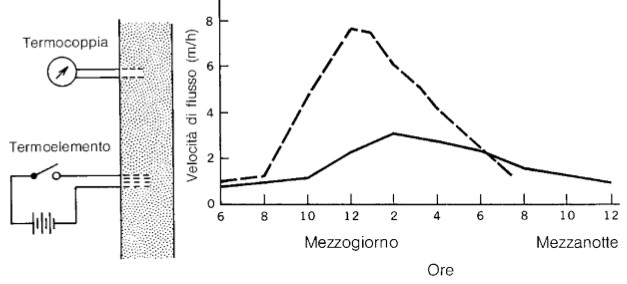
\includegraphics[scale=0.5]{immagini/velocita.jpg}
\caption{Misurazione della velocità di flusso della linfa xilematica}
\end{figure}

Che succede se non abbiamo traspirazione?

Viene tagliato il fusto e si ha trasudazione di liquido xilematico.

\subsection{Pressione radicale}
La radice genera pressione positiva richiamando ioni dal suolo e concentrandoli nello xilema:
\begin{itemize}
\item{Abbassamento di $\Psi_{s}$ nello xilema}
\item{Richiamo di acqua e aumento di $\Psi_{p}$ }
\end{itemize}
La pressione radicale può essere misurata recidendo la radice alla sua emergenza dal suolo e applicando un tubo capillare che ha mercurio all'estremità: dal movimento del mercurio si vede la pressione.

Gli ioni richiamati dal suolo alle cellule dell'endoderma permettono il richiamo di acqua: questi ioni infatti non possono tornare indietro, si accumulano e quindi aumenta il potenziale di pressione, generando una pressione positiva (effetti non rilevabili).
Nell'embolia, quando le bolle di aria sotto tensione tendono a dilatarsi, sentono questa pressione positiva e questa controbilancia la tensione che dilaterebbe l'espansione della bolla, comprimendola ed evitanto l'embolia.

Di notte c'è ampia disponibilità di acqua, la pressione radicale spinge l'acqua all'interno dei vasi e questa può uscire dalla pianta per il fenomeno di \emph{guttazione} (non è rugiada, ma acqua). L'acqua di guttazione fuoriesce sulla superficie fogliare all'estremità del fascio vascolare che percorre la lamina fogliare in cativà, o \emph{idatodi}, che sono pori che permettono l'espulsione di acqua.


\section{Traspirazione stomatica}
L'acqua che si trova allo stato di vapore negli spazi intercellulari della foglia esce per diffusione attraverso gli stomi (traspirazione stomatica).

Gli stomi, localizzati sulla faccia ventrale della foglia, possono essere aperti o chiusi: ciò regola la traspirazione. A questo livello la pressione idrostatica è:
\begin{equation}
\centering
P = -\frac{2T}{r}
\end{equation}
dove r è il raggio di curvatura del menisco che si forma e T la tensione superficiale.
Con l'aumentare della traspirazione, la pellicola sulla superficie si assottiglia e va ad abbracciare le singole fibrille: aumenta quindi l'entità della pressione idrostatica negativa. Con la diminuzione del raggio di curvatura, si ha aumento del valore assoluto della pressione idrostatica.
La traspirazione avviene negli spazi interni agli stomi (camere sottostomatiche), ma la pianta traspira anche attraverso le superfici della foglia rivestite di materiale idrofobo, che rallenta il passaggio di acqua. 

Tutte le parti aeree della pianta sono rivestite di sostanze idrofobe per evitare l'eccessiva traspirazione.
Esistono aperture sul tronco, o \emph{lenticelle}, che attraversano la corteccia: non sono soggette a regolazione, gli stomi si.

I fattori determinanti la traspirazione sono:
\begin{enumerate}
\item{Gradiente della pressione del vapore acqueo: più è ripido , più veloce è la diffusione dell'acqua dal mesofillo all'atmosfera}
\item{Resistenze alla diffusione del vapore acqueo: strato di aria ferma sulla superficie della foglia e chiusura stomi}
\end{enumerate}

\begin{figure}[H]
\centering
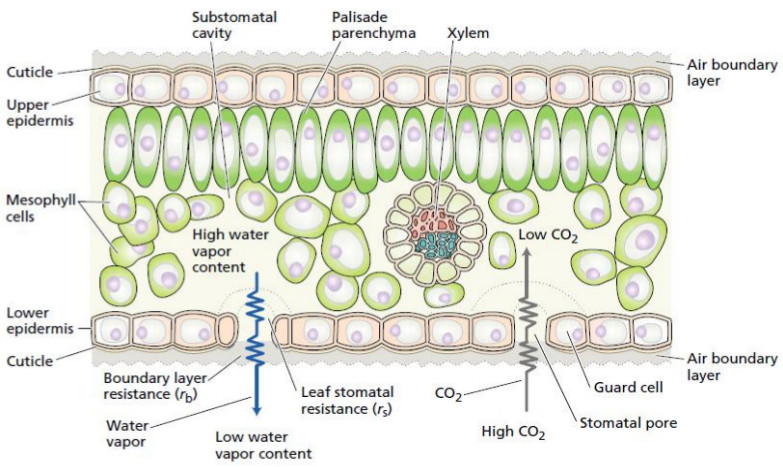
\includegraphics[scale=0.5]{immagini/stomi.jpg}
\caption{Percorso dell'acqua nella foglia. L'acqua è spinta dallo xilema nella parete cellulare del mesofillo, dove evapora negli spazi aeriferi della foglia. Il vapore acqueo diffonde verso l'esterno, attraverso le aperture stomatiche, mentre la $CO_{2}$ percorre la via opposta}
\end{figure}
Umidità relativa \lfreccia misura della concentrazione del vapore acqueo in diversi ambienti, riferendoci alla pressione parziale del vapore acqueo in codizioni di saturazione.

Resistenza dello strato limite \lfreccia varia con lo spessore dell'aria immobile sulla superficie della foglia. Esso dipende dalla velocità del vento, dall'anatomia fogliare e dall'orientamento della lamina fogliare. Può controllarlo la pianta andando incontro a modificazioni strutturali, ad esempio aumentando i peli in prossimità dello stoma: questi intrappolano aria ed evitano turbolenze: anche altre modificazioni tipo l'invaginazione degli stomi, modificazioni nella disposizione della foglia per esporle meno ai movimento dell'acqua.

Resistenza stomatica fogliare \lfreccia apertura stomatica regolata in base alle esigenze metaboliche della pianta: aumentando l'apertura, aumenta la traspirazione. Controllo poco efficiente se la resistenza dello strato limite diminuisce troppo in base alla ventilazione sulla foglia della pianta :  maggiore traspirazione con maggiore ventilazione.

\subsection{Stomi}

Nelle monocotiledoni hanno la parte centrale assottigliata e le parti periferiche più spesse (a manubrio). La parte scura corrisponde a deposizione di grosse quantità di microfibrille di cellulosa. Ci sono due \emph{cellule di guardia} e due \emph{cellule sussidiarie}, che aiutano le cellule di guarda nell'apertura/chiusura degli stomi.

Nelle dicotiledoni si ha lo stoma classico.

A livello dell'epidermide, le cellule di guardia sono le uniche verdi (in grado di effettuare fotosintesi); le cellule sussidiarie sono immerse nelle cellule dell'epidermide.
\begin{figure}[H]
\centering
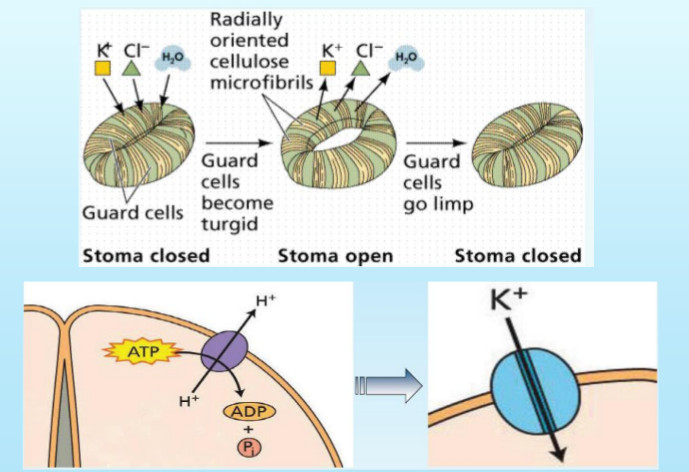
\includegraphics[scale=0.5]{immagini/chiusura.jpg}
\caption{Chiusura/apertura stomatica}
\end{figure}
 
Le microfibrille di cellulosa ispessiscono la parete delle cellule di guardia : funzionale all'apertura stomatica.
Gli stomi sono numerosi, ma l'area che occupano è molto limitata, ma distribuita in piccole aree della foglia: vantaggioso rispetto all'avere un unico grande poro, perchè la traspirazione è molto più rapida. Quando l'acqua si sposta alla periferia del poro, il suo movimento è più facilitato perchè da un lato mancano le interazioni con le cellule dintorno. 

Le cellule di guarda fanno gonfiare lo stoma, ma la tensione non è uniforme: quella sul lato interno è molto maggiore di quella sul lato esterno.
Le cellule sussidiarie forniscono ioni ed acqua, riducendo il proprio volume e facendo espandere le cellule di guardia: il K entra grazie ad un canale ionico sulla membrana, attivato da un'ATPasi (depolarizza la membrana, attivando il canale per K, che entra dentro la cellula).	

La variazione di turgore delle cellule di guardia è causata dall’ingresso massivo di ioni potassio (da 0,2 a 0,6 M) dalle cellule compagne e successivamente di acqua. L’ingresso del potassio è attivo ed è determinato dalla pompa protonica di membrana (iperpolarizzazione e apertura canali voltaggio dipendenti). L’assorbimento di cloro o la sintesi di anioni come il malato sono finalizzati a neutralizzare la carica del potassio. La chiusura stomatica si realizzerebbe per inversione dei suddetti processi.

(15.10.2014)
\paragraph{Recapitolando...}
Conseguenza dell'apertura stomatica è la perdita di acqua ad opera del processo di traspirazione. 
La regolazione dell'apertura stomatica dipende da vari fattori: variazione del turgore delle cellule di guardia, movimento di ioni.

\subsection{Andamento dell'apertura stomatica}
La fase oscura della fotosintesi, che è la fase di vera e popria sintesi, è diversa nei vari tipi di pianta. Il metabolismo di base è quello C3; piante che vivono in particolari ambienti adottano un meccanismo accessorio, che è il C4 per piante che vivono in climi caldi e umidi, e il CAM, tipico delle crassulacee, piante grasse, adattate a vivere in estrema aridità ed elevate temperature. Le piante CAM e C4 devono limitare fortemente la traspirazione: stomi chiusi durante il giorno e aperti durante la notte, acquisiscono la $CO_{2}$ nella notte, la immagazzinano fissandola e la rilasciano il giorno. 
Per una pianta C3, l'apertura stomatica varia in questo modo: stomi chiusi la notte, si aprono rapidamente all'nizio della gironata e si mantengono aperti in modo costante, poi iniziano  achiudersi nel pomeriggio e stanno chiusi tutta la notte. Nelle ore più calde si può avere parziale chiusura degli stomi.

Le condizioni che regolano l'apertura stomatica somno fattori esterni ed interni: luce, temperatura, disponibilità di $CO_{2}$ nel tessuto fotosinteticamente attivo e le condizioni di idratazione della pianta.
 
La luce controlla indirettamente il processo attraverso gli effetti che ha sull'utilizzo di $CO_{2}$: ad elevata isolazione, elevato consumo di $CO_{2}$ \lfreccia apertura stomatica.
Il meccanismo di apertura stomatica sembra coinvolgere gli ioni Ca e l'acido abscissico, ma non si hanno dati certi di quale siano gli eventi che portano dall'abbondanza di $CO_{2}$ all'apertura stomatica.

L'effetto diretto sull'apertura lo ha la luce blu, ovvero quella delle prime ore dell'alba, che modula l'apertura degli stomi dopo la chiusira notturna: è coinvolto un pigmento, la \emph{zeaxantina} (famiglia xantofille), che agisce insieme a fotorecettori che percepiscono la luce blu, i \emph{criptocromi} e le \emph{fototropine} \lfreccia a stomi chiusi, l'irradiazione con luce blu porvoca l'apertura. C'è una coincidenza dello spettro d'azione dell'apertura stomatica con quello di assorbimento della zeaxantina (non coincidono perfettamente perchè gli esperimenti fatti in vitro utilizzano pigmenti puri, che in vivo puri non sono).
La concentrazione di zeaxantina nelle cellule di guardia è correlata con l'intensità della luce blu fornita.

\paragraph{Come agisce la zeaxantina?}
I mutanti NPQ1 sono mutanti nell'enzima che converte la violaxantina in zeaxantina: questi pigmenti amplificano, nello spettro della radiazione luminosa, la capacità di percezione della luce solare nel cloroplasto, e percepiscono radiazioni luminose che proteggono le clorofille dall'ossidazione. Sono presenti nel cloroplasto e interconvertiti da una serie di enzimi cme NPQ1; queste due molecole sono precursori dell'acido abscissico. 
\begin{figure}[H]
\centering
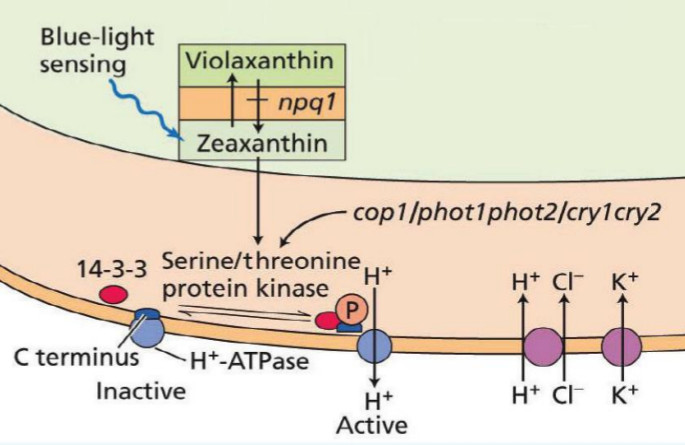
\includegraphics[scale=0.4]{immagini/zea.jpg}
\caption{Azione della zeaxantina}
\end{figure}

L'identificazione di questo mutante ha permesso di identificare la zeoxantina come una \emph{molecola fondamentale nella regolazione del processo di apertura stomatica}.
La zeaxantina regola l'apertura stomatica attivando la pompa protonica ATPasi mediante fosforilazione dei residui di Ser e Tre del dominio regolatorio della poma protonica (tramite ser/tre chinasi) alla quale si lega anche la proteina 14-3-3 \lfreccia pompaggio all'esterno di H+ e richiamo all'interno della cellula di ioni K+, e così di ioni Cl \lfreccia riarrangiamento della permeabilità della membrana plasmatica e accumulo di ioni \lfreccia apertura stomi.
La zeaxantina aumenta con la stimolazione da parte della luce blu.

Lo stress idrico, se è forte nel suolo, viene compensato da un sistema di regolazione mediato dall'acido abscissico (ABA). Se il suolo è scarsamente idratato, stomi aperti presto la mattina, a mezzogiorno si chiudono: a seconda dell'idratazione; in suolo molto secco gli stomi si chiudono completamente e si riaprono la mattina successiva; se il suolo non è molto secco, dopo la chiusura di mezzogiorno gli stomi si riaprono nelle ore meno calde e si richiudono la sera.

\subsection{Acido abscissico (ABA)}
È l'\emph{ormone dello stress} che protegge la pianta dallo stress idrico. Come tutti gli ormoni vegetali, viene sintetizzato a tutti i livelli della pianta (negli animali ci sono le ghiandole), in particolare nei cloroplasti della foglia, a partire dalla zeaxantina. Le concentrazioni degli ormoni vegetali sono sempre molto basse e gli effetti sono locali e regolati dalla capacità di percezione dei segnali dei vari distretti in cui arrivano, nonchè dal metaoblismo.

È un acido, può essere più o meno dissociato. Lo stroma del cloroplasto è BASICO: ABA è deprotonato (ABA-), quindi non può attraversare liberamente le membrane. Durante stress idrico, il pH dello stroma si inacidisce: ABA protonato, permea attraverso le membrane, diffonde attraverso il coloplasto delle cellule di guardia e ne raggiunge la membrana, attivando vari processi tra cui l'attivazone della pompa protonica.
Favorisce la chiusura stomatica al momento dello stress idrico.

\chapter{Nutrizione minerale}

Comprende i fenomeni di acquisizione di nutrienti dall'ambiente. Le piante organicano C, N, S e captano dal suolo tutti gli elementi necessari per la sopravvivenza (sempre che il suolo ne contenga).

Un nutriente essenziale è un componente intrinseco nel metabolismo della pianta, la cui assenza causa severe anormalità nella crescita, sviluppo o riproduzione della pianta.

Sachs : sviluppo coltura in soluzione, detta \emph{coltura idroponica}, che individua alcuni elementi essenziali alla crescita elle piante. 

Un sistema di coltura utilizzato è il \emph{terreno di Hoagland}, che contiene tutti i nutrienti inorganici necessari alla pianta a completare un ciclo vitale .
\begin{figure}[H]
\centering
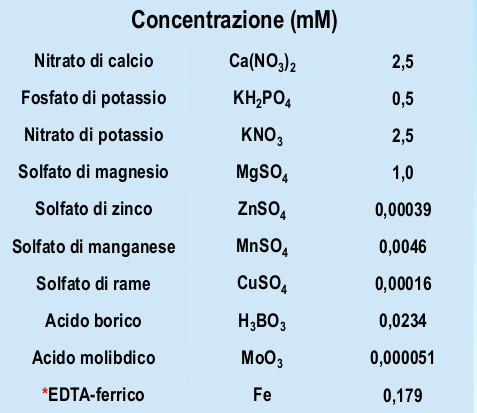
\includegraphics[scale=0.4]{immagini/hoagland.jpg}
\caption{Composizione del terreno di Hoagland}
\end{figure}
 Il ferro viene fornito sotto forma di metallo chelato con EDTA, perchè altrimenti ossida e forma sali e idrossidi che non possono essere assimilati nelle piante.
Un terreno del genere ci consente di fare esperimenti per vedere se un certo nutriente è un elemento essenziale per la pianta (cosa che sarebbe difficile da vedere sperimentalmente lasciando le piante nel suolo).
 
La \emph{coltura idroponica} prevede:
\begin{itemize}
\item{Immersione radici in acqua}
\item{Circolazione di nutrienti}
\item{Fornire nutrienti sempre in concentrazioni adeguate}
\item{Vasche forate per impedire la formazione di alghe che possono utilizzare nutrienti che ci sono nella soluzione}
\item{Cambiare spesso la soluzione di nutrienti perchè il pH può variare \lfreccia i nutrienti sono dispoibili a secondo del pH del mezzo in cui sono presenti}
\end{itemize}

\begin{figure}[H]
\centering
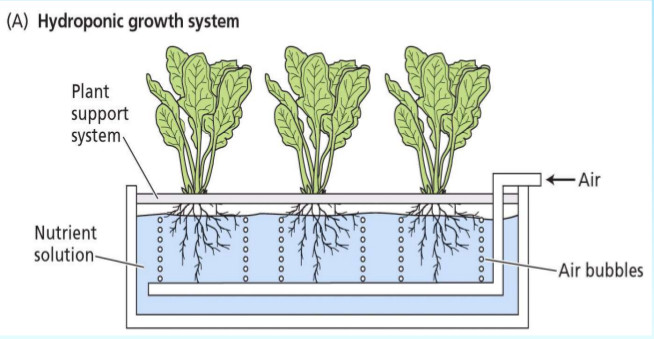
\includegraphics[scale=0.4]{immagini/idroponica.jpg}
\caption{Coltura idroponica}
\end{figure}
Le piantine, sostenute dal supporto, hanno le radici libere di crescere nel mezzo liquido. La soluzione deve essere aerata per evitare l’anossia, che inibirebbe la respirazione delle cellule della radice e la conseguente captazione di
nutrienti. Il contenitore in cui si effettua la coltura liquida ha di solito le pareti dipinte in nero per impedire la
penetrazione della luce. Quest’ultima favorirebbe infatti la crescita di alghe che competerebbero per i nutrienti con la pianta. Infine la soluzione nutriente deve essere cambiata spesso per evitare variazioni di pH del mezzo e fenomeni di carenza dovuti all’eccessivo assorbimento di alcuni nutrienti.

La \emph{coltura su pellicola nutritiva} prevede che le radici ricevano un ampio apporto di ossigeno:
\begin{figure}[H]
\centering
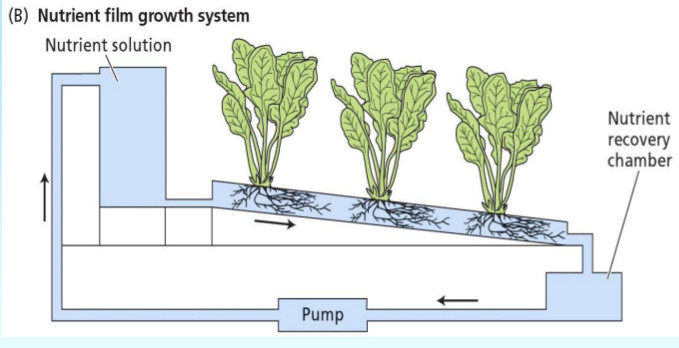
\includegraphics[scale=0.4]{immagini/pellicola.jpg}
\caption{Coltura su pellicola nutritiva}
\end{figure}
Le piante sono cresciute su di un tubo inclinato in cui viene pompata di continuo la soluzione nutritiva. Le radici
crescono nella parte basale del tubo, dove sono continuamente bagnate da una sottile pellicola di soluzione
nutriente aerata. E’ il metodo più usato nella produzione commerciale di piante.

La \emph{coltura aeroponica} prevede che la soluzione di crescita venga vaporizzata tramite un sistema di ventilazione. Le radici sono sospese in aria e vengono continuamente spruzzate con la soluzione nutriente;
\begin{figure}[H]
\centering
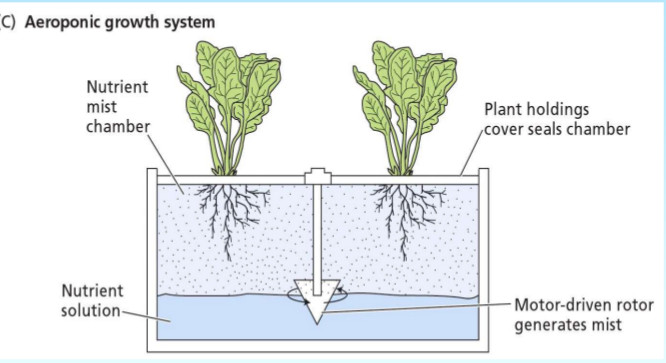
\includegraphics[scale=0.4]{immagini/aeroponica.jpg}
\caption{Coltura aeroponica}
\end{figure}
Questo approccio consente una facile manipolazione dell'ambiente gassoso intorno alle radici, ma richiede un più alto livello di nutrienti.

\paragraph{Applicazione fogliare} è effettuata spruzzando una soluzione contenente elementi nutritivi sulle foglie. In tal modo
l’assorbimento è più rapido ed elimina problemi di assorbimento non specifico di un nutriente da
parte delle particelle del suolo. L’assorbimento di un nutriente è ottimale se la soluzione forma una
sottile pellicola sulla foglia. Per ottenere ciò si aggiungono alla soluzione detergenti in grado di
ridurre la tensione superficiale. Le soluzioni nutritive penetrano soprattutto attraverso la cuticola.
Queste applicazioni non possono tuttavia sostituire del tutto l’assorbimento radicale e pertanto
sono indicate allorché quest’ultimo è reso difficoltoso da stress, infezioni, traumi radicali ecc.

(20.10.2014)
\section{Carenze nutritive}
Quando un elemento minerale viene fornito in concentrazioni inadeguate ad una
pianta si manifestano sintomi di carenza, come conseguenza di uno scompenso
nutrizionale. In coltura idroponica un sintomo è facilmente collegabile con la
carenza di un elemento minerale, mentre in natura è molto difficile capire la natura
del sintomo in quanto anche agenti microbiologici possono determinare alterazioni
che assomigliano a carenze.
I sintomi della carenza di un elemento nutritivo risultano dal suo insufficiente
rifornimento e sono collegati al ruolo svolto da tale elemento nel metabolismo.
Spesso un elemento minerale svolge una o più funzioni nella pianta, così
schematizzabili:
\begin{itemize}
\item{Costituente di composti}
\item{Attivatore di enzimi}
\item{Osmoregolatore}
\end{itemize}

Per trattare le carenze nutrizionali, si usa la \emph{concimazione}:
\begin{itemize}
\item{Concimi chimici : Contengono in genere sali di macronutrienti (azoto,
fosforo e potassio) miscelati insieme oppure contengono uno solo dei
suddetti sali. Meno comune è invece la concimazione con micronutrienti
che possono essere aggiunti se il suolo ha una carenza preesistente in
micronutrienti}
\item{Concimi organici : Contengono gli elementi nutritivi sotto forma di
molecole organiche che pertanto dovranno essere degradate a minerali dai
microrganismi del terreno}
\end{itemize}

Determinazione degli elementi minerali nei tessuti vegetali:ù
\begin{enumerate}
\item{Metodo della digestione : una volta raccolti i tessuti, vengono mineralizzati in presenza di acido formico, che li degrada nei componenti essenziali}
\item{Metodo dell'incenerimento : il tessuto raccolto viene essiccato (a 90/100\textcelsius), fino a che il tessuto non viene ridotto in cenere. C e H vengono misurati effettuando incenerimento in una corrente di $O_{2}$: si legano all'$O_{2}$ e il contenuto viene stimato misurando il vapore, l'acqua e la $CO_{2}$ che si forma}
\end{enumerate}
La carenza di \emph{Silice} nel suolo è drammatica per la pianta: gli steli vengono indeboliti \freccia allentamento: la pianta (in questo caso le Graminacee) cade al suolo e si perde il prodotto della pianta. Il \emph{silicio} è importante anche come deterrente per gli erbivori.
Con questi metodi rileviamo anche la più piccola quantità di minerali.
 
Il \emph{Sodio} è importante per le piante a metabolismo CAM e C4, ma non è un elemento essenziale.

I micronutrienti, anche se a bassa concentrazione, devono essere presenti nella pianta affinchè essa possa compiere il proprio ciclo vitale.

Il \emph{Nichel} è importantissimo: nel seme, è presente in concentrazioni estremamente basse, ma già adeguate allo sviluppo dell'intera pianta. Esso non può essere studiato in coltura idroponica.

Per quanto riguarda lo studio delle necessità mnutrizionali della pianta, ci sono difficoltà per caratterizzare ciò che è essenziale per la pianta; è stata necessaria una \emph{classificazione} a vari livelli (ruolo biochimico):
\begin{itemize}
\item{Gruppo 1 : nutrienti che fanno parte di composti con C. Troviamo N e S, componenti delle proteine}
\item{Gruppo 2 : elementi che sono fondamentali nei processi di produzione e conservazione di energia e struttura. Troviamo P, Si e B. (Il Silicio non è considerato strettamente essenziale per tutte le piante, es serve come difesa per le graminacee)}
\item{Gruppo 3 : nutrienti la cui funzione in forma ionica può contribuire alla osmoregolazione. Troviamo K, Cl, Ca, Mg, Mn, Na}
\end{itemize}
Se sono essenziali, questi elementi \underline {devono} essere presenti nel suolo in quantità adeguate alla crescita della pianta. La loro disponibilità è legata alle caratteristiche del suolo. La crescita della pianta, la produzione di biomassa sono influenzate da questa disponibilità: si ha aumento della crescita o della resa con l'aumentare dei nutrienti essenziali, fino a che non viene raggiunta la \emph{concentrazione critica}. A questo punto la pianta si trova in una zona "adeguata" alla sua crescita. Si osserva che i macronutrienti hanno un range più ampio per quanto riguarda la \textbf{zona di adeguatezza}. Poi si arriva alla zona in cui il nutriente diventa \emph{tossico}. 
Al di sotto della concentrazione critica, la pianta cresce secondo le sue possibilità, poi la pianta cresce in modo adeguato fino a che i nutrienti diventano tossici.
\begin{figure}[H]
\centering
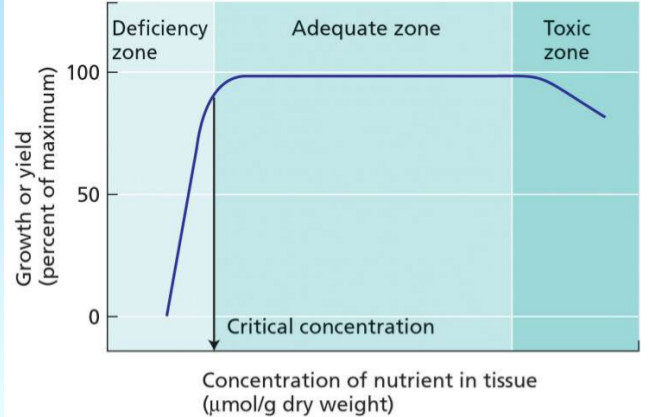
\includegraphics[scale=0.3]{immagini/carenza.jpg}
\caption{Andamento generale della crescita in un tessuto vegetale in funzione della concentrazione di un nutriente. La
concentrazione critica è quella a cui si ha la riduzione del 10\% della crescita }
\end{figure}
La carenza di nutrienti si manifesta con varie alterazioni: i sintomi però spesso non sono tali da discriminare la carenza di un certo nutriente. Per vedere i sintomi, si usa una pianta di controllo e altre piante dalle quali si elimina un nutriente \lfreccia si manifesta sempre una ridotta crescita. Può manifestarsi anche una carente attività fotosintetica (foglie gialle, risultanti dai pigmenti che emergono più mascherati dal verde della clorofilla. Ciò deriva da carenza di Fe e di N: entrambe servono alla clorofilla perchè fanno parte della molecola stessa).

Nella \emph{pianta del tabacco}, il Ca, che ha effetti importanti nello stabilizzare il fuso mitotico, comporta riduzione della crescita. 

\subsection{AZOTO}
Contenuto nella maggior parte dei concimi, insime a P e K (concimi NPK). 
L'azoto è un componente di proteine, aa, lipidi; fa parte degli anelli pirrolici della clorofilla. Nonostante sia presente in grandi quantità nell'atmosfera, in realtà nel suolo è presente, ma non sempre facilmente disponibile per le piante. Viene assorbito in 3 forme:
\begin{enumerate}
\item{Nitriti : facilmente solubili nel suolo e disponibil, vengono convertiti in ammonio}
\item{Nitrati : facilmente solubili nel suolo, sono la forma più comunemente assimilata. Convertiti in nitriti e poi ammonio}
\item{Ammonio : preferito, ma non sempre è disponibile in questa forma. L'ammonio entra a far parte direttamente della coppia di reazione del ciclo di  (??)\todo{cerca} sintasi, che porta all'incorporazione dell'ammonio negli aa Glu e Gln}
\end{enumerate}
La scarsa disponibilità di N nel suolo non sussiste per alcune piante che riescono a fissare l'azoto gassoso, poichè hanno sviluppato simbiosi con batteri azotofissatori del suolo. In queste piante le carenze di azoto sono rare!
Gli effetti della carenza sono molteplici: ridotta crescita, ridotta capacità fotosintetica.

Gli elementi minerali, una volta incorporati, a livello delle foglie, tramite la circolazione floematica, vengono mobilizzati componenti dei tessuti, tra cui quelli minerali. a seconda della mobilità dell'elemento, se c'è carenza può venire messo in circolo nel floema per degradazione di tessuti che lo contengono nella pianta adulta, e reso disponibile per la foglia giovane. 

Molti elementi non possono essere mobilizzati e sono definiti \emph{immobili}: sono spesso quelli che si trovano nelle foglie giovani.
L'azoto è un elemento mobile.

(22.10.2014) 
\section{Macronutrienti}
\subsection{Fosforo}
Disponibile in fosfato, la forma che le piante prediligono. In suoli basici o neutri prevalgono le altre due forme.
Il fosfato può essere assorbito dalla decomposizione della sostanza organica: vengono resi così più facilmente disponibili per la pianta. Vengono secrete delle fosfatasi che facilitano il distacco dei fosfati dalla sostanza organica in decomposizione, rendendolo disponibile per la pianta.

È presente in condizioni limitanti, quindi può limitare la crescita della pianta.
Gli zuccheri fosfati sono intermedi di \emph{respirazione} e \emph{fotosintesi}.
I sintomi di carenza sono legati ad una ridotta crescita della pianta nell'apice vegetativo (i fosfati fanno parte di commposti essenziali strutturali) con aumentato accrescimento radicale grazie alla simbiosi con batteri.

\subsection{Potassio}
Presente nel suolo sotto forma di catione ed è un importante osmoregolatore cellulare. In concentrazioni non limitanti la crescita. Entra o esce per determinare gonfiamento o sgonfiamento delle cellule di guardia degli stomi.

\subsection{Zolfo}
Assorbito sotto forma di solfati derivati o dalla ossidazione di anidridi solforose o da decomposizione della sostanza organica. Oltre a far parte della struttura delle proteine, è importante per la determinazione della loro struttura terziaria. Importante per la regolazione del potenziale REDOX per la pianta e presenza in composti antiossidanti (glutatione e proteine ferro-zolfo).

\subsection{Calcio}
Presente in concentrazioni elevate nel suolo e a livello dell'apoblasto, a livello della lamella mediana, dove funge da collante tra le molecle di acidi pectici esterificandosi con queste molecole e dando struttura alla lamella mediana. Nella cellula è relegato nel vacuolo e funge da messaggero vegetale per la percezione della gibberellina.
È poco mobilizzabile per le foglie giovan, come zolfo e magnesio.

\subsection{Magnesio}
La carenza di magnesio è disastrosa perchè il Mg struttura la clorofilla (gli anelli pirrolici sono coordinati con la clorofilla): si ha clorosi e degenerazione del cloroplasto.
Ha altre fuznioni: regolazioe di attività enzimatiche fondamentali (attivatore di alcuni enzimi della fotosintesi), legame di ATP ad enzimi che lo utilizzano come fonte di energia-

\section{Micronutrienti}

\subsection{Ferro}
Il ferro è nel suolo sotto forma di ossidi, insolubili. La pianta lo acquisisce sotto forma di ione ferrico e in forma chelata, che fa si che il ferro si trovi in forma ionica, impedendo la formaizone degli ossidi.
Le funzioni del ferro sono molte, poichè esso è in gradi di passare a due stati di ossidazione diverse. Nonostante che il ferro non entri a far parte direttamente delle molecole di clorofilla, è in qualche modo coinvolto nella sa sintesi, perchè la clorofilla è carente in piante che vivono in suoli poveri di ferro (clorosi ferrica).

\subsection{Boro}
Presente come acido borico: struttura della parete, legandosi a zuccheri e pectine, poi sintesi di acidi nucleici e di ormoni. Se manca, la pianta cresce in maniera stentata: forse perchè non si sintetizza bene a parete e perchè la distensione della pianta è promossa dall'auxina, un ormone.

\subsection{Rame}
Prelevato dal suolo come catione $Cu^{2+}$. Sa passare da più stati di ossidazione, coinvolto in regolazione potenziale redox e presente in enzimi che catalizzano reazioni redox, in enzimi che fanno parte di \emph{reazioni di detossificazione}.

\subsection{Zinco}
In forma ionica nel suolo, coinvolto nella regolazione di enzimi fotosintetici e respiratori, coinvolto nella \emph{sintesi della clorofilla}.

\subsection{Manganese}
Presente come ione manganese, la funzione è legata all'attivazione e regolazione di enzimi come le decarbossilasi o le deidrogenasi. In particolare, ha ruolo fondamentale nel processo di \emph{fotolisi dell'acqua}.
Fa parte di un complesso proteico che contiene 4 atomi di Mn che strappano 4 protoni e 4 elettroni da una molecola d'acqua.

\subsection{Molibdeno}
È fondamentale per l'attività di nitrogenasi e nitrato reduttasi, essenziali per l' \emph{assimilazione dell'N}. La nitrato reduttasi produce nitriti da nitrati; la nitrogenasi è fondamentale per la fissazione dell'azoto atmosferico ed inorganico che si trova nel suolo; nelle piante superiori non è funzionale, nelle simbiosi e nelle piante inferiori si.

\subsection{Cloro}
Disponibile come $Cl^{-}$, funziona spesso da controione per il K nella membrana (osmoregolatore) ed è coinvolto nella reazione di \emph{fotolisi dell'acqua} e nella \emph{divisione cellulare}. Carenze di cloro sono visibili come ridotta attività dei meristemi.

\subsection{Nickel}
Cofattore dell'enzima ureasi,  ma la funzione nelle piante non è ben chiara. I livelli di Nickel nella pianta sono bassissimi, spesso quelli intrinseci nella pianta bastano, non serve assimilarlo.

\section{Trasporto cellulare}
Come arrivano i nutrienti alla cellula vegetale?

Una volta in soluzione acquosa, gli elementi del suolo vengono caricati nello xilema e diffondono nella pianta. Arrivati alla banda del capsari e poi all'endodermide con l'acqua, si ha una selezione degli ioni che sono presenti nell'acqua: inserimento nella membrana plasmatica di trasportatori, modulatori del trasporto degli ioni come canali per acqua (acquaporine), traslocatori ecc.

Per vedere il risultato dell'azione dei trasportatori, si usa una cellula gigante di un'alga verde, che ha tutti i trasportatori tipici delle piante, e si impiegano microelettrodi per ogni ione che ci permettono di misurare l'accumulo ionico, ovvero la concentrazione all'interno della cellula. Grande vacuolo con citoplasma in periferia. Si immergono le cells in soluzione di K, Na e Cl e coi microelettrodi si misurano le concentrazioni di ioni nei vari compartimenti: accumulo del potassio nel citoplasma e nel vacuolo (e anche per Na e Cl). Il trasporto è diverso nei due compartimenti.

Notiamo una capacità del sistema di trasporto di distinguere questi ioni e di accumularli a livelli diversi. I rapporti tra K e Na in citoplasma e vacuolo sono diversi.

Mais e fagiolo: monocotiledone e dicotiledone.

(27.10.2014)
\subsection{Cinetiche di trasporto}
Quando l’assunzione di uno ione da parte della radice viene monitorata in presenza di concentrazioni
crescenti di ioni nel mezzo esterno, la curva che correla l’assunzione con la concentrazione può essere
formalmente descritta dall’equazione di Michaelis-Menten. A concentrazioni esterne di KCl fino a 0.5
mM, il tasso di assunzione di K+ di radici di orzo raggiunge un plateau a circa 0.2 mM. A concentrazioni
molto superiori di KCl (1-50 mM) il tasso di assunzione subisce un ulteriore incremento.

Ci sono due tipi di cinetiche: la \emph{cinetica di Michaelis e Menten} e la \emph{cinetica bifasica}.

Non tutte le molecole che entrano nella cellula hanno un sistema a bassa e alta affinità di trasporto. La cellula vegetale è caratterizzata da memebrana semipermeabile: entrambi i tipi di membrana hanno i loro trasportatori.

Nel citosol tra interno e esterno esiste una differenza di potenziale per cui l'interno è  negativo e misura -120 mV: presenza di protoni all'esterno della cellula. Il tonoplasto funziona  all'opposto del plasmalemma, acidifica il vacuolo (vacuolo ha pH 5,5 come apoplasto) il che è fondamentale per l'attività di enzimi nel vacuolo. Il vacuolo ha anche ruolo di \emph{stoccaggio delle cariche}. 
\begin{figure}[H]
\centering
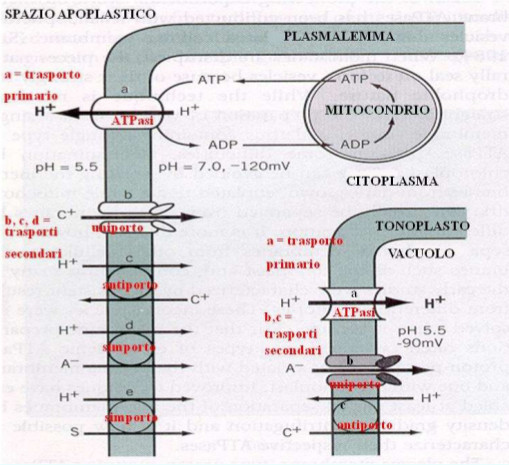
\includegraphics[scale=0.4]{immagini/trasporto.jpg}
\caption{Rappresentazione schematica del trasporto ionico nella radice}
\end{figure}
La pompa protonica ATPasica funziona usando l'energia prodotta nel mitocondrio: in base al gradiente protonico che stabilisce si formano dei trasporti primari che poi possono attivare trasporti secondari.
Il saccarosio è prodotto dalla fotosintesi e va caricato nel floema per essere distribuito a tutti i settori della pianta.

\subsection{Un caso particolre: il ferro}
Nel suolo il Fe si trova principalmente come $Fe^{3+}$, praticamente insolubile a pH neutri o alcalini.
$Fe^{2+}$ è più solubile e maggiormente assorbito dalle piante, ma a pH 6-8, tipico dei terreni
neutri, è ossidato a $Fe^{3+}$.
La concentrazione di Fe inorganico totale in soluzione è $10^{-7}$M-$10^{-23}$M (pH 3.5 e 8.5).
È un micronutriente, ma è indispensabile per le piante. Purtroppo è carente nella maggior parte dei suoli e si trova prevalemtnemente come ferro ferrico. 
Nei suoli alcalini ha pochi protoni, si formano idrossidi e si ossidano e formano ferro non assimilabile dalle piante. 

Nel suolo il Fe è presente anche sotto forma di \emph{chelato} ad acidi organici (citrato,
malato, tartrato) o altre sostanze organiche prodotte dai microrganismi del suolo
o dalla degradazione della sostanza organica. Anche questa forma di Fe è presente ad una concentrazione troppo bassa per le necessità delle piante.

La concentrazione ottimale di ferro nel suolo dovrebbe essere $10^{-4}$-$10^{-9}$ M. Le piante usano due distinte strategie prima per solubilizzare e poi per assorbire il Fe dal suolo:
\begin{itemize}
\item{Strategia I: riducente (dicotiledoni e monocotiledoni non graminacee)}
\item{Strategia II: chelante (graminacee)}
\end{itemize}

\begin{figure}[H]
\centering
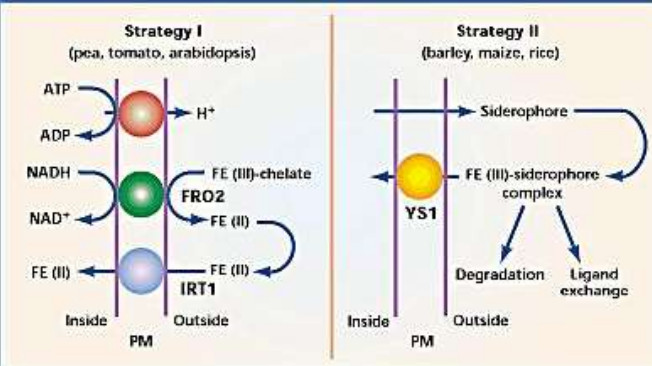
\includegraphics[scale=0.4]{immagini/strategie.jpg}
\caption{Strategie per l'assimilazione del ferro}
\end{figure}

\paragraph{Strategia I} 
la carenza di Fe induce il gene che codifica per pompa protonica ATPasica, determinando grande rilascio protoni nell'apoplasto e determinandone acidificazione. 
Induce anche il gene che codfica per \emph{ferrico reduttasi}, enzima di memebrana che catalizza la riduzione dei chelati a chelati di ferro (chelazione ferro ferrico disponibile da acidificazione del suolo con molecole organiche a loro volta secrete dalla pianta) \lfreccia chelanti legano il ferro ferrico e formano dei chelati che rilasceranno il ferro sotto forma ferrosa dall'azione riducente della ferrico reduttasi. Usa NADPH che viene ridotto a NADP+ ossidando il ferro. Il ferro è rilasciato nella radice, è assorbito dalla pianta e un trasportatore (sintesi indotta da basi livelli ferro nel suolo) acquisisce ferro ferroso e lo trasporta all'interno della cellula. 

\paragraph{Strategia II} non si ha acidificazione suolo corrispondente a una riduzione dei livelli ferro nel suolo. Comporta la sintesi di molecole come amminoacidi e proteine in carenza di ferro: \emph{fitosiderofori}, sono forti chelanti per il ferro ferrico e competono con particelle suolo a cui il ferro si lega, e ne provocano il distacco.
 
Il trasportatore specifico  (YS1) nella cellula  trasloca intracellularmente il complesso ferrosideroforo, il complesso si stacca nel citosol e il ferro viene reso disponibile, ma prima viene reso ferro ferroso. Il sideroforo può essere riusato. 

\paragraph{}

I fotosiderofori derivano da via biosintetica che parte dalla metionina. La via metabolica per la sintesi dei  fitosiderofori è in comune con l'etilene. 

\section{Assorbimento degli ioni}
L'acquisizione dei nutrienti minerali dipende sia dalla capacità di assorbimento, sia
dalle caratteristiche di accrescimento dell'apparato radicale.
La radice si accresce in continuazione al fine di
allontanarsi dalle zone di esaurimento nutritivo e
“colonizzare” zone di terreno più ricche in minerali.

Abbiamo una \emph{radice a fittone} (soprattutto nelle dicotiledoni) e un \emph{radice fascicolata} (monocotiledoni, da radice primaraia originano dallo stesso punto radici secondarie lunghe più o meno tutte uguali) rappresentate nell'immagine. 
\begin{figure}[H]
\centering
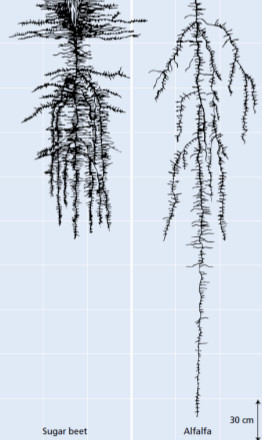
\includegraphics[scale=0.4]{immagini/fittone.jpg}
\caption{Radice fascicolata (sx) e a fittone (dx)}
\end{figure}

La radice tende a crescere per evitare zone prive di alimenti che sono prossime alla radice. 
In un suolo asciutto la radice tende a ridurre il proprio accrescimento verticale in favore di un allungamento laterale; a volte crescono per arrivare a zone non più aride. In un suolo irrigato si accresce in profondità.

La radice regola il suo accrescimento in base ai nutrienti disponibili nel suolo. 
Un esempio sono le
radici “mazzetto” delle Betulaceae e Fabaceae in
suoli poveri di $PO_{4}^{3-}$.
Queste
radici
si
sviluppano
negli
strati
superficiali, perché servono soprattutto per
assorbire $PO_{4}^{3-}$ dilavato dai residui organici
accumulati sulla superficie del terreno. Esse incrementano l'assorbimento.

\section{Interazioni radici-batteri}
Esistono e sono funzionali alla capacità della pianta di assorbire nutrienti particolarmente carenti nel suolo. I \emph{noduli radicali} sono strutture che si differenziano a seguito di penetrazione di nutrienti.

La rizosfera ospita una grande varietà di microrganismi, che possono essere più o meno
importanti per la pianta, dal punto di vista ecofisiologico.
Batteri e funghi possono invadere le radici dell'ospite o vivere nel terreno, e traggono nutrimento da essudato che la pianta emette a livello della rizosfera.

Le interazioni radici-funghi (micorrizze) sono le più diffuse: interessano l'80\% delle specie studiate e tutte quelle di interesse economico. Molte micorrize sono specie-specifiche nei confronti dell'ospite. Sono associazioni mutualistiche di tipo simbiotico. Si distinguono in:
\begin{itemize}
\item{Micorrize ectotrofiche (ectomicorrize): fungo sia nel tessuto che nella cellula, stabilendo un rapporto molto stretto con il citosol}
\item{Micorrize endotrofiche (endomicorrize): fungo fuori dalla pianta, non penetra nelle cellule, solo nei tessuti}
\end{itemize}

Il fungo acquisisce nutrimento dalla pianta e la pianta acquisisce più capacità di assorbire i nutrienti.

\paragraph{Ectomicorrizze}
L'ifa fungina avvolge l'apice radicale e qualche ifa si accresce e penetra nel rizoderma senza però addentrarsi nell'endoderma e nei fasci vascolari. L'ifa forma il rivestimento all'apice radicale che di fatto sostituisce l'apparato assimilatore: la radice perde la cuffia a protezione del meristema, l'apice diviene più arrotondato, vengono persi i peli radicali la cui funzione è sostituita da ife fungine. Le ife fungine si ramificano e costituiscono il \emph{reticolo di harting} che si muove a livello dell'apoplasto tra una cellula e l'altra senza comunque mai penetrare. 

Le specie interessate sono numerosissime : specie arboree che vivono in regioni temperate o fredde, gimnosperme, angiosperme olmi, betulle ecc.

Sono solo due le famiglie di funghi interessate a questa simbiosi: \emph{attino miceti} e \emph{basiliomiceti}.


\paragraph{Endomicorrizze}
Sono prevalentemente effettuate da funghi delle Endomonacee che non hanno un corpo fruttifero ma il micelio che si accresce nel suolo, viene a contatto con la pianta e si accresce. L' ifa si accresce nel pelo radicale, penetra \emph{nel} tessuto vegetale, ma i due citosol non vengono mai a contatto. L'ifa si ramifica aumentando  la superficie di contatto costituendo un \emph{arbuscolo} e delle vescicole in cui ci sono \emph{spore} che costituiscono fase sessuale del ciclo fungino. Si parla di VAM, vescicolo-arbuscolare.

La capacità di assorbimento è  additiva rispetto alle endomicorrizze. Non c'è modificazione dell' apparato radicale a occhio nudo e non scompaiono peli radicali: la capacità di assorbimento della pianta è sommata a quella del fungo. Sono le piu antiche ed hanno una grande distribuzione nelle piante.

\paragraph{}
Altre endomicorizze: nelle Eritacee (vescicole arbuscolari) e nelle Orchidacee (assimilazione nutrienti da parte del seme che non ha adeguata apposizione nutrienti dalla madre).
favorisce assimilazione di nutrienti piu ccarenti nel suolo. simbiosi quasi assenti in suoli ben concimati. se fungo si attacca alla pianta dove i nutrienti cono cmq presenti, allora diventa una forma di parassitismo da parte del fungo.  
\subsection{Ruoli fisiologici}
 Lo sviluppo della simbiosi micorrizica aumenta notevolmente l'accrescimento della pianta, grazie alla maggiore disponibilità di nutrienti minerali (P, N, K). Substrati di crescita concimati con alte dosi di P inibiscono o eliminano la micorriza (il fungo può anche diventare parassita).
\begin{itemize}
\item{Le micorrize espandono notevolmente la zona di esaurimento nutritivo: le ife estendono
l'apparato radicale dell'ospite}
\item{Per la pianta può essere vantaggioso cedere assimilati al fungo, piuttosto che utilizzarli per
accrescere il proprio apparato radicale}
\item{Forse le micorrize ectotrofiche che si sviluppano nella fase organica del terreno ne idrolizzano il
fosfato e lo trasferiscono all'ospite}
\end{itemize}

L'assimilazione del fosfato crea grandi problemi per le piante che vivono in suoli acidi e non favoriscono la solubilizzazione del fosfato. Il fungo qui è molto utile perchè degrada con una \emph{fosfatasi} il fosfato organico della materia organica, accumula fosfato come polifosfati organici in granuli, percorre le ife e raggiunge le parti radicali della pianta, dove vengono idrolizzati polifosfati e recupera fosfato organico per il proprio metabolismo.   
 
\section{Ciclo biogeochimico dell'azoto}
L'azoto non può essere assimilato dalle piante come forma gassosa, va convertito in forme diverse. L'azoto atmosferico è la fonte principale di azoto del ciclo biogeochimico e può, attraverso conversione, essere inserito nella composizione della sostanza organica. 

I processi di fissazione rompono il triplo legame di $N_{2}$ per convertirlo: ciò richiede molta energia. Ci sono \emph{tre processi fondamentali} del ciclo biogeochimico di N:
\begin{enumerate}
\item{Fissazione atmosferica : energia dai fulmini. Conversione di azoto molecolare in nitrato }
\item{Fissazione biologica : batteri nel suolo che convertono l'azoto molecolare in ammonio}
\item{Fissazione industriale : usata per produrre concime agricolo, converte azoto molecolare in ammonio}
\end{enumerate}
\begin{figure}[H]
\centering
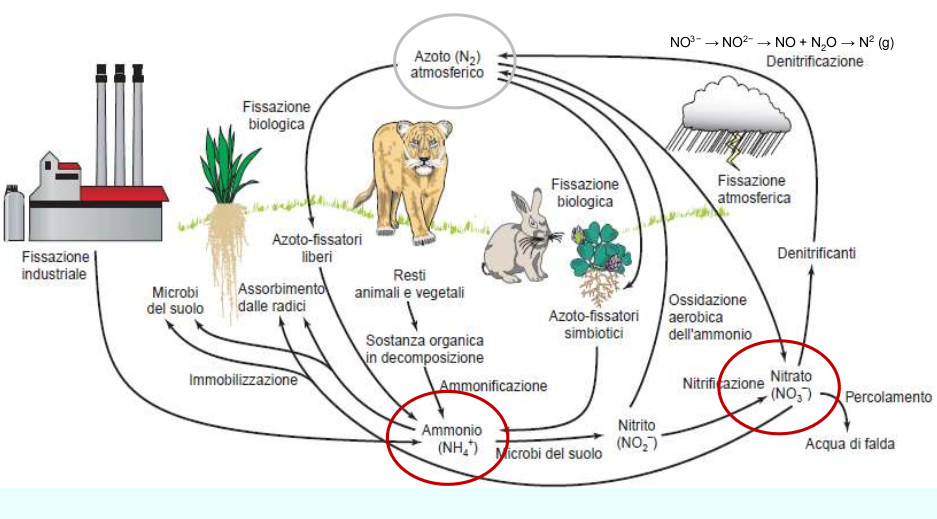
\includegraphics[scale=0.4]{immagini/ciclo.jpg}
\caption{Ciclo biogeochimico dell'azoto}
\end{figure}
Per ridurre azoto atmosferico ad ammonio-nitrito-nitrato servono trasformazioni biologiche e decomposizione sostanza organica. Il nitrato può infatti derivare da microbi del suolo e  da processi naturali.   
 

\subsection{Assimilazione dell'N}
\begin{itemize}
\item{Ammonio direttamente incorporato negli aa, traslocato nella cellula e mediante una serie di reazioni entra a far parte di \emph{glutammina} e \emph{glutammato} e da qui è organicato} 
\item{Il nitrato ha via più lunga: una volta nella cellula va ridotto a nitrito, il quale poi è ridotto ad ammonio in un reazione che avviene nel plastidio e nel cloroplasto. Una volta ridotto, mediante l' attività di due enzimi è convertito ad ammonio e può poi entrare nella composizione degli amminoacidi}
\end{itemize} 
 \begin{figure}[H]
\centering
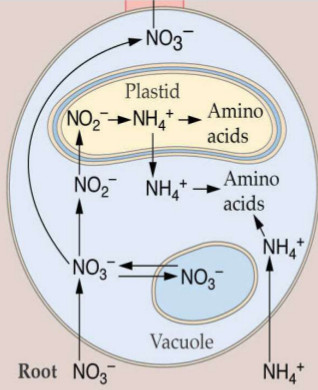
\includegraphics[scale=0.35]{immagini/azoto.jpg}
\caption{Assimilazione dell'azoto}
\end{figure}
 
Elevate concentrazioni di ammonio sono tossiche per le piante. Pertanto l’ammonio in eccesso deve essere rapidamente convertito in aminoacidi o immagazzinato nel vacuolo. 
 
  
(29.10.2014)

L'azoto circola nel ciclo biogeochimico in forma bimolecolare.
La conversione in forma organica avviene anche grazie all'azione dell'uomo (es per i concimi); sia nella forma di ammonio, nitrato o nitriti può essere assimilato dalle piante, che lo organicano e lo rilasciano nell'atmosfera; batteri nitrificanti nell'atmosfera lo rendono di nuovo inorganico e dispinibile nel suolo.

Le piante contribuiscono all'organicazione dell'azoto: esse riescono a sintetizzare tutti gli aa essenziali che posssono essere usati dagli animali, che non possono fare altrettanto.
Il nitrato, una volta entrato nella cellula vegetale, viene convertito in ammonio (che è tossico, quindi si ha riduzione ad opera della Nitrato reduttasi e della nitrito reduttasi); l'ammonio è substrato di glutammato sintetasi e glutammina sintetasi, che incorporano l'N negli aa.
Questi enzimi sono presenti in varie isoforme. Parte dell'azoto può essere elaborato  nella radice per fornire composti che fanno crescere la radice stressa.

Anche l'ammoniaca è tossica per la pianta: nella cellula si trova in un ambiente basico, con ioni OH che si legano all'ammonio generando ammoniaca non carica. Ciò riduce di fatto il pH del citosol. A pH acido, l'ammoniaca si protona. 
\section{Assorbimento dell'azoto}
Le piante hanno sviluppato dei sistemi di trasporto di queste molecole, altamente specifici e costitutivi, localizzati nel plasmalemma e nella membrana vacuolare. 

L'ammonio viene quindi conservato nel vacuolo. Lo ione ammonio è assorbito da specifici trasportatori (uniporto cationico) costitutivi presenti sul plasmalemma delle cellule dell’epidermide (rizoderma) della radice. Tali trasportatori sono ad alta affinità e con cinetica saturabile.

2 tipi di trasportatori:
\begin{enumerate}
\item{AMT1;1, AMT1;3 e AMT1;5 \lfreccia traslocano l'ammonio dalle parti più esterne della pianta. Sono localizzate nell'epidermide radicale e traslocano ammoniaca per via simplastica}
\item{AMT1;2 \lfreccia si trova a livello del parenchima corticale, tasporta ammonio per via apoplastica o simplastica}
\end{enumerate}
 
\subsection{Assorbimento del nitrato}
Non crea problemi alla pianta, ma all'uomo si: ecco perchè è vietato concimare con questo composto.
\begin{figure}[H]
\centering
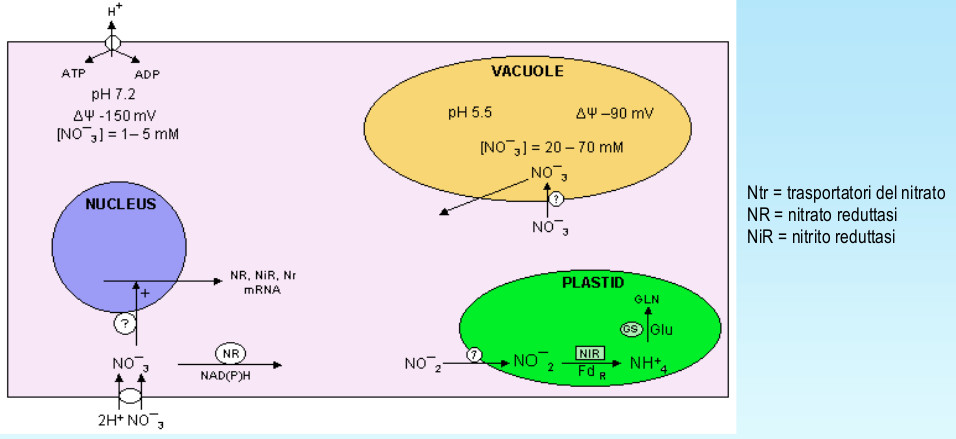
\includegraphics[scale=0.4]{immagini/nitrato.jpg}
\caption{Assorbimento del nitrato}
\end{figure}
 
La cellula vegetale che deve produrre molti aa ha bisogno di nitrato: cotrasporto con $H^{+}$, 2 protoni per molecola di nitrato: si ha una parziale temporanea depolarizzazione della membrana perchè c'è una temporanea disclocazione di carica.
La $H^{+}$-ATPasi di membrana pompa ioni H+ fuori dalla cellula, producendo un gradiente elettrico e di pH. I trasportatori di nitrato cotrasportano nella cellula due o più H+ per ogni $NO_{3}^{-}$. Il nitrato può essere trasportato attraverso il tonoplasto e conservato nel vacuolo. Nel citosol, il nitrato viene ridotto a nitrito, che entra nel plastidio dove viene ridotto ad ammonio. L'ammonio è fissato nel glutammato a dare glutammina mediante l'azione della GS\footnote{Glutammina sintasi}. Il nitrato funziona da segnale per aumentare l'espressione della nitrato reduttasi, della nitrito reduttasi e dei geni Ntr.

A differenza dell’ammonio le piante possono accumulare elevate quantità di nitrato e traslocarlo da un organo all’altro senza manifestare inconvenienti. Tuttavia se tali piante sono per uso alimentare risultano tossiche poiché $NO_{3}^{-}$ è convertito nel fegato a $NO_{2}^{-}$ che si lega alla Hb rendendola incapace di fissare l’$O_{2}$. L’eccessiva concimazione con nitrato è quindi da evitare in agricoltura.

\paragraph{Trasportatori del nitrato} piante trattate con nitrato radiattivo per periodi diversi e a concentrazioni diverse potevano reagire in due modi diverso:
\begin{figure}[H]
\centering
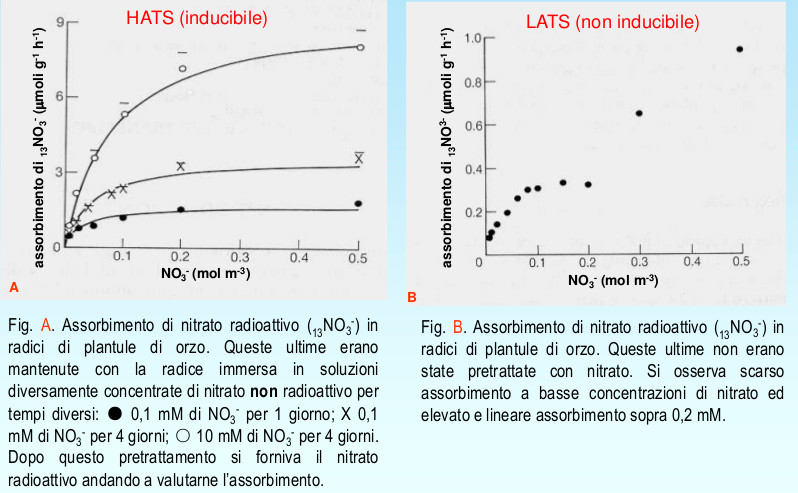
\includegraphics[scale=0.43]{immagini/trasporto1.jpg}
\caption{Trasporto del nitrato}
\end{figure}
 
Esisitono quindi due sisitemi:
\begin{enumerate}
\item{HATS: ad \emph{alta affinità}, con cinetica saturabile}
\item{LATS: a \emph{bassa affinità}. Anche in grandi quantità di azoto, non si ha saturazione (solo a 50mM, che è tantissimo!!!) e cinetica lineare che si mantiene tale fino a 50 mM}
\end{enumerate}
Si distinguono una frazione costitutiva (LATS) e una inducibile (HATS). Si crea così una forte flessibilità di assorbimento dell'azoto. Possiamo ben vedere qui le due cinetiche: una bifasica (LATS) e l'altra di Michaelis e Menten (HATS) già descritte nel paragrafo 3.4.1.

N.B. Anche HATS può essere una frazione costitutiva, se la concentrazione dello ione è circa 1 mM,

L'assimilazione dell'azoto, sia nitrato che ammonio, avviene sia a livello della radice che dell'apparato vegetativo: nello xilema si trovano diversi composti che sono intermedi dell'assimilazione dell'azoto, nitrato ed aa. 
Questa variabilità è dovuta al fatto che i sistemi enzimatici per l'assimilazione dell'azoto si trovano sia nella radice che nell'apparato vegetativo.

Nella foglia, questi enzimi sono localizzati a livello del cloroplasto e l'azoto viene assimilato con modalità simili alla radice.

(3.11.2014)
\subsection{Riduzione del nitrato}
Il nitrato viene ridotto prima a nitrito e poi ad ammonio. 

Abbiamo il trasferimento di 8 elettroni dall'azoto all'ammoniaca \freccia $\Delta G$ molto alto! È una reazione complessa, formata da reazioni che non avvengono spontaneamente.

La conversione da nitrato a nitrito avviene nel citosol. 
A seconda della specie, nello xilema troviamo diversi livelli di nitrato e di nitrato organicato. Il nitrito è tossico e viene subito traslocato dentro il plastidio, che contiene l'apparato enzimatico necessario per convertire il nitrito in ammoniaca (nitrito reduttasi) ed incorporarla in $\alpha-chetoglutarato$ per produrre glutammina. 
La conversione da nitrato a nitrito avviene tramite reazione con NADH e \textbf{nitrato reduttasi}: si produce nitrito e NAD+.
\begin{equation} 
NO_3^{-} + NADH + H^{+} \lfreccia (NO_{2})^{-} + NAD^{+} + H_{2}O
\end{equation}

Viene utilizzato alternativamente NADH o NADPH se ci troviamo rispettivamente nel cloroplasto o nel plastidio.

La \emph{nitrato reduttasi} utilizza NADH e NADPH nel citosol e NADH nelle cellule verdi. L'enzima impiega 3 gruppi prostetici: un \emph{FAD}, un \emph{citocromo b557} e un complesso del \emph{molibdeno}. È un omodimero che contiene questi gruppi prostetici: il FAD lega all'estremità C-terminale il NADH, prende un elettrone e lo passa all'eme e poi al complesso del molibdeno, che lega il nitrato e lo riduce. È localizzata nel citoplasma delle cellule parenchimatiche clorofilliane e delle cellule del rizoderma e del parenchima radicale. Nella radice il donatore di
elettroni è sia il $NADH_{2}$ che il $NADPH_{2}$.
\begin{figure}[H]
\centering
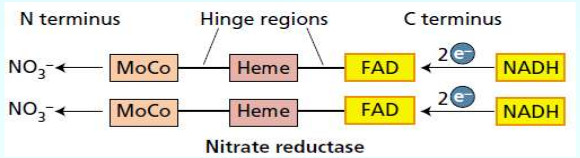
\includegraphics[scale=0.43]{immagini/nitrato_reduttasi.jpg}
\caption{Azione della nitrato reduttasi}
\end{figure}

La regolazione è fine e specifica, e regola anche l'enzima \textbf{nitrito reduttasi} che converte il nitrito in ammonio: è inibito dalla fosforilazione e stimolato dai livelli di nitrato (substrato).
\paragraph{}
La \emph{nitrito reduttasi} catalizza la riduzione del nitrito ad ammonio con il trasferimento di 6 elettroni, grazie alla \emph{ferridossina ridotta}. La ferridossina è un segnale di attività fotosintetica in corso e della presenza di equivalenti riducenti e di scheletri carboniosi, sui quali l'azoto ridotto potrà essere incorporato nella sintesi degli amminoacidi: è ridotta quando la fotosintesi è attiva (nella fase luminosa produce NADPH, che a sua volta riduce la ferridossina e produce equivalenti riducenti).

Nei tessuti non fotosintetizzanti, la ferridossina viene rigenerata dal NADPH proveniente dai pentoso fosfati.
La ferridossina ridotta cede 6 elettroni al nitrito \lfreccia si ottiene ammoniaca.

La struttura dell'enzima prevede la presenza di componenti in grado di trasferire elettroni, come il $Fe^{2+}$: è presente un \emph{gruppo ferro-zolfo} e un \emph{eme}. Gli elettroni vengono trasferiti al centro ferrozolfo, poi all'eme e infine al nitrito con produzione di ammonio.
\begin{figure}[H]
\centering
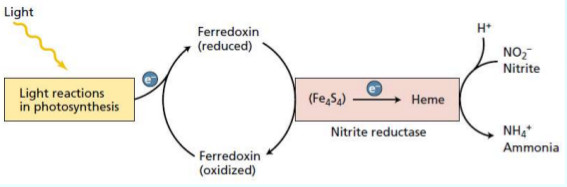
\includegraphics[scale=0.53]{immagini/nitrito_reduttasi.jpg}
\caption{Azione della nitrito reduttasi}
\end{figure}
La nitrito riduttasi (64 KDa) catalizza la riduzione del nitrito ad ammonio. È localizzata nei cloroplasti delle cellule del
parenchima fogliare e nei plastidi delle cellule della radice. Nei tessuti fotosintetici la Fd-ossidata viene ridotta grazie al
trasporto fotosintetico di elettroni. Nelle radici la Fd-ossidata viene rigenerata dal NADPH prodotto dalla via dei pentosi fosfati.

\paragraph{Regolazione del processo}
La nitrato reduttasi è attivata dalla luce, dai carboidrati e dal nitrato. L'ammonio, il buio e il glutammato la inibiscono.
\begin{figure}[H]
\centering
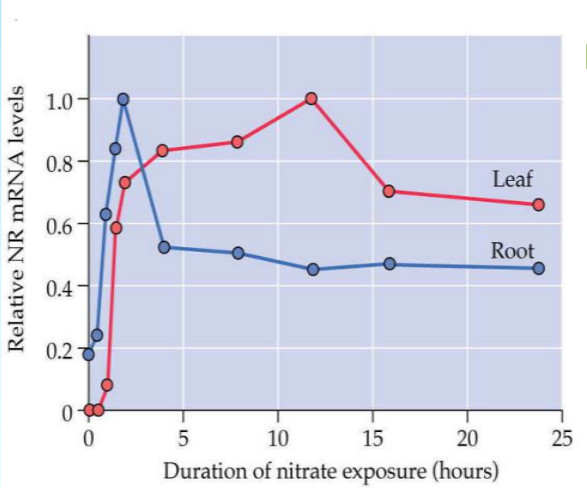
\includegraphics[scale=0.3]{immagini/regolazione.jpg}
\caption{Regolazione della nitrato reduttasi attraverso l'espressione genica}
\end{figure}
Piante di pochi giorni deprivate di nitrato e poi esposte ad alti livelli di nitrato mostrano un'iniziale assenza della nitrato reduttasi, poi un picco degli mRNA di questo enzima, poi un calo per quanto riguarda la radice, in cui il nitrato permane per un tempo breve, mentre resta costante nella foglia, dove la fissazione del nitrato resta costante grazie al continuo apporto di nitrato dallo xilema. Stessa cosa per la luce.

Fattori che fungono da attivatori hanno un effetto meno diretto sulla sintesi dell'enzima, ma controllano l'attività dell'enzima stesso attraverso la sua fosforilazione: quello che attiva la nitrato reduttasi promuove anche una fosfatasi che defosforila dei residui di serina in prossimità del molibdeno; fattori che inibiscono l'enzima attivano una chinasi che fosforila questi residui di Ser. Questo tipo di controllo avviene anche negli mRNA ed è più rapido, a seconda delle esigenze della pianta e della disponibilità del nitrato nel suolo.

La regolazione principale è proprio sulla nitrato reduttasi: la nitrito reduttasi è scarsamente oggetto di regolazione a livello della sua espressione o della sua attivazione.

\subsection{Assimilazione dell'ammoniaca: ciclo GS-GOGAT}
La seconda metà del processo di assimilazione dell'azoto prevede \emph{l'incorporazione dell'ammoniaca negli amminoacidi}. La glutammina sintetasi (GS) e la glutammato sintasi (GOGAT) sono gli enzimi chiave.

L'azoto ammoniacale viene legato ad un chetoacido con la formazione dell'aa corrispondente (intervengono le trasnaminasi).
Inizialmente si pensava che questa reazione fosse ad opera della \textbf{glutammato deidrogenasi} , che (de)amina il glutammato, provocando la sintesi di $\alpha$-chetoglutarato :

\begin{itemize}
\item{Forma NADH dipendente nei mitocondri}
\item{Forma NADPH dipendente nei cloroplasti}
\end{itemize}

I ruoli specifici di queste GDH non sono ben chiari. Si pensa che possano funzionare principalmente
nel catabolismo del glutammato (deaminazione).
Ci sono problemi relativi a questo enizma:
\begin{itemize}
\item{Ha affinità molto bassa per l'ammonio. Km tra i 5 e i 50 mM, è altissima (concentrazioni non tossiche di NH4+ tra 0,2 ed 1 mM).}
\item{Catalizza una reazione reversibile che può rilasciare ammonio \lfreccia enzima non adatto a catalizzare la sintesi di Glu nelle piante.}
\end{itemize}

La GS catalizza, a spese di un ATP, l'incorporazione dello ione ammonio sul Glu: si forma glutammina. La glutammina, con l'$\alpha$-chetoglutarato, è substrato della GOGAT, che trasferisce il gruppo amminico all'$\alpha$-chetoglutarato: si formano 2 Glu (uno derivante dalla deaminazione della Gln e uno dall'amminazione dell'$\alpha$-chetoglutarato).

La GOGAt impiega equivalenti riducenti derivati dal NADPH o dal NADH o dalla ferridossina ridotta. Questi enzimi hanno varie isoforme nei tessuti.
Alla fine, una molecola di Glu viene utilizzada dalla Gln per l'organicazione di un'altra molecola di ammonio \lfreccia si produce un solo Glu.

La GS impiega ATP derivante dalla fotosintesi e richiede per l'attivazione uno ione bivalente come mangesio o manganese o cobalto. 
\begin{figure}[H]
\centering
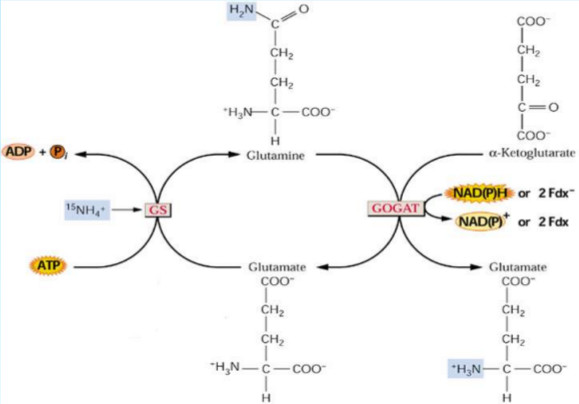
\includegraphics[scale=0.4]{immagini/ciclo1.jpg}
\caption{Ciclo GS-GOGAT}
\end{figure}

La struttura è complessa, in quanto costituita da 8 subunità identiche e grandi. Le isoforme sono 2:
\begin{enumerate}
    \item{Plastidiale \lfreccia assimila l'azoto per la sintesi di aa per lo sviluppo locale della radice; la forma clorosplastica ha la funzione legata all'assimilazioe di un ammonio che deriva dalla fotorespirazione, processo tipico del cloroplasto che utilizza ossigeno per bruciare il carbonio. L'ammonio prodotto è tossico e quindi viene usato.}
    \item{Citosolica \freccia produzione di Gln per il trasporto a lunga distanza: viene esportata nel floema e traslocata ai tessuti, a seconda della specie.}
\end{enumerate}

La GOGAT viene attivata dalla Gln, anche in basse concentrazioni. La Km per l'ammonio è $10^{-5}$. È formata da 8 subunità.
La forma NADH-GOGAT si trova nelle radici ed organica l'azoto per l'utilizzo in loco e per il trasporto a lunga distanza. 

Una forma di NADH-GOGAT si trova nei vasi floematici ed organica l'ammonio che arriva o dalle radici o dalle foglie senescenti (foglie mature che vanno incontro a morte). A livello dei fasci vascolari delle foglie, seve per la riassimilazione della Gln mobilizzata dalle foglie senescenti.

La forma Fd-GOGAT si trova nei cloroplasti del germoglio dove serve per il metabolismo dell’azoto liberato durante
la fotorespirazione oppure si trova nei plastidi delle radici di piante nutrite con nitrato.
\subsection{Sintesi di amminoacidi}
Le piante sono capaci di generare tutti i 20 aminoacidi proteici. Esse sintetizzano inoltre molti altri (circa 200)
aminoacidi non proteici. La sintesi dell’aspartato è effettuata dall’aspartato aminotransferasi in figura. Un’altra
transaminasi, la alanina aminotransferasi, trasforma l’acido glutammmico e l’acido piruvico in alanina e acido 2-
oxoglutarico.
Una volta che Glu e Gln sono stati sintetizzati, sono diponibili gruppi amminici per sintetizzare tutti gli altri amminoacidi.

Il primo enzima è l'\textbf{aspartato aminotrasferasi} : trasferimento di un gruppo amminico su una molecola di ossalacetato, sintetizzando aspartato e rigenerando ossalacetato e $\alpha$-chetoglutarato. L'Asp viene usato per sintetizzare Asn, per trasferimento del gruppo amminico della Gln sull'Asp da parte dell'\textbf{asparagina sintetasi}: si formano Asn e Glu. L'asparagina è l'aa con più alto rapporto di atomi di C e di N, e per questo viene utilizzato per lo stoccaggio dell'azoto e per il suo trasporto all'interno della pianta. Asn è abbondante nei noduli (nella radice) delle piante che formano simbiosi con i batteri azotofissatori. È un amminoacido fortemente coordinato con l'attività fotosintetica:

\paragraph{Esperimento} in piante con Asp wt e altre senza Asp. Al buio, si ha una forte induzione della sintesi dell'asparagina, proprio perchè sintesi di C organiico e assimilazione di N sono fortemente coordinate. Se la pianta al buio riesce ad assimilare N, lo farà sull'Asn; alla luce, è favorita la sintesi degli altri aa perchè vengono sintetizzate grandi quantità di cheletri carboniosi.

\subsection{La fissazione biologia dell'azoto}
Le piante sono in grado di utilizzare l'azoto che viene fissato in ammoniaca a partire da N molecolare atmosferico da parte di diversi organismi. 
La fissazione biologia è analoga alla sintesi chimica, ma lo strumento è diverso in quanto le condizioni sono diverse: la reazione avviene a T ambiente in ambiente acquoso, grazie all'enzima \textbf{nitrogenasi}. L'energia della reazione viene dall'ATP e dal potere riducente (trasferimento di 8 elettroni all'N molecolare per diventare N ammoniacale).

Gli organismi che operano la fissazione biologica sono procarioti, che possono vivere liberi nel suolo o formare simbiosi con le piante. Ci sono i cianobatteri (aerobici) e altri batteri che possono essere anche anaerobi o anaerobi facoltativi: importante perchè \emph{la nitrogenasi è fortemente inibita dall'ossigeno}. 

Si sono evoluti meccanismi per escludere l'ossigeno dalla nitrogenasi, in maniera tale da mantenerla attiva: es. nel nodulo radicale c'è un meccanismo fisico di impermeabilizzazione per l'ossigeno; \emph{Vulnera} vive con un simbionte e sviluppa delle strutture a livello delle foglie, delle \emph{vescicole che escludono l'ossigeno}.
Nel riso, alla fine del suo ciclo riproduttivo, e quando l'allagamento ritira, le comunità di Azolla e Anabena (cianobatterio con cui Azolla fa simbiosi) seccano: visto che Anabena permette la fissazione di grandi quantità di N, alla senescenza della felce si rilascia nell'ambiente una forma di concimazione azotata organica. C'è una cellula nel cianobatterio, \emph{l'eterocisti}, che è impermeabile all'ossigeno; la pianta inoltre non presenta il fotosistema II.

La \textbf{nitrogenasi} è inattiva a basse temperature; è un enzima molto antico costituito da 2 proteine, che funziona solo se esse sono associate:
\begin{itemize}
    \item{Reduttasi \lfreccia presenta 32 atomi di ferro e contiene un centro Fe-molibdeno fondamentale per la catalisi enzimatica.}
    \item{Reduttasi della reduttasi \lfreccia rigenera la proteina I. Due subunità identiche fra loro }
    \end{itemize}
    La nitrogenasi effettua 8 cicli per ridurre una molecola di $N_{2}$. Ogni ciclo inizia con la riduzione della proteina 2, che lega 2 ATPMg e si complessa con la proteina 1 trasferendole l’elettrone. Il complesso proteina 1-2 si disfa ed il ciclo si ripete con le modalità prima descritte. Nei primi due cicli si forma $H_{2}$, mentre nei successivi 6 cicli si formano 2 $NH_{3}$. La durata degli 8 cicli è 1.25 secondi, un tempo decisamente molto alto che denota l’arcaicità di questo enzima. Gli equivalenti riducenti (ovvero gli elettroni) sono ottenuti dalla ferridossina.
    
La catalisi prevede 8 cicli lenti (1,25 s), inizia con il legame di ATP alla proteina II che permette il cambiamento conformazionale per il legame della ferridossina e l'associazione delle due proteine; attraverso i centri ferrozolfo e ferromolibdeno gli elettroni sono trasferiti alla proteina 1 e poi all'N. Nei primi due cicli viene prodotto $H_{2}$, gli altri producono ammoniaca.

\subsection{L'eterocisti delle alghe azzurre}
\begin{figure}[H]
\centering
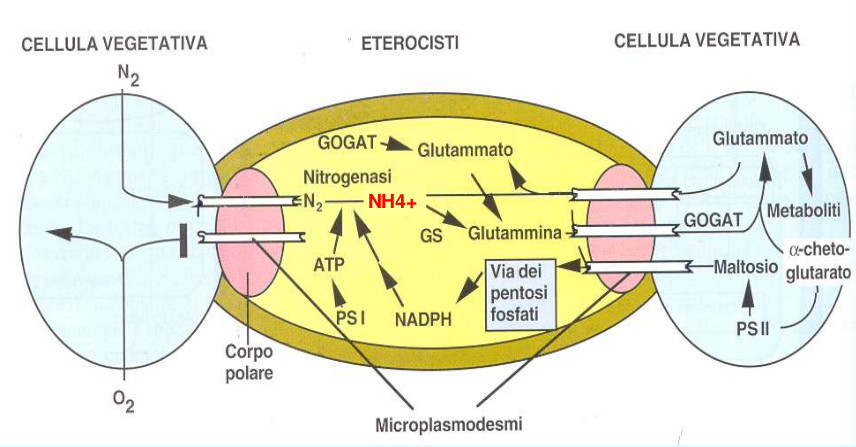
\includegraphics[scale=0.35]{immagini/eterocisti.jpg}
\caption{Rappresentazione schematica degli scambi di carbonio ed azoto tra eterocisti e cellule vegetative}
\end{figure}
 L’eterocisti, essendo priva di PSII, non produce ossigeno e zuccheri con la fotosintesi. Di conseguenza gli zuccheri, sotto forma di maltosio, sono forniti dalle cellule vegetative. Tali zuccheri servono attraverso la via del pentoso fosfato a formare NADPH e quindi ferredossina ridotta (Fdred) che fornirà gli elettroni alla nitrogenasi. L’ATP è prodotto con la fotofosforilazione ciclica. L’ammoniaca, derivante dalla riduzione dell’azoto, è assimilata dalla glutammina sintetasi.
La glutammina prodotta è trasportata alle cellule vegetative dove è trasformata in glutammato dalla glutammato
sintetasi.

L'eterocisti è a contatto con le due cellule vegetative adiacenti, ha un triplo rivestimento che impedisce l'accesso all'ossigeno nell'eterocisti stessa. La cellula vegetativa adiacente è permeabile all'ossigeno, ha un metabolismo completo e non differenziato. Cellula vegetativa ed eterocisti sono sia a contatto, ma la permeabilità è tale che l'ossigeno non riesce a passare; inoltre, pur avendo un apparato fotosintetizzante, questo è modificato: ce n'è uno solo dei due (fotosistema 1) affinchè non si produca ossigeno, si mantiene la parte funzionale alla fissazione dell'azoto e si elimina quella che produce ossigeno. Esiste solo il fotosistema 1, che nella fotosintesi produce equivalenti riducenti, ovvero riduce NADP+ a NADPH; in questo caso si limita a produrre ATP. Gli equiovalenti riducento sono prodotti dlla via dei pentoso fosfati a partire dal maltosio, la forma di carbonio organicata che viene trasferita all'eterocisti ed ossidata.

L'eterocisti ha un differenziamento tale per cui questa cellula non può più riprodursi per via vegetativa. Viene però sviluppata solo quando l'azoto ambientale è presente in condizioni limitanti. L'azoto deve permeare a partire dall'assorbimento fatto dalle cellule vegetative adiacenti, e trasferito all'eterocisti tramite un piccolo plasmodesma.

La glutammina sintetasi incorpora l'ammonio nell'$\alpha$-chetoglutarato e così lo toglie dal citoplasma: viene prodotta glutammina ed utilizzata dalla GOGAT per produrre glutammato.

(5.11.2014)
\section{La fissazione azotata nelle Leguminose}
Le piante superiori riescono ad acquisire l'azoto grazie alle simbiosi con azotofissatori: es. Leguminose e batteri Rizobium.
Questa simbiosi si trova in almeno il 90\% delle leguminose. Le simbiosi si formano a livello delle radici, e si vedono come ispessimenti: a questo livello la radice prolifera e produce una ammasso cellulare all'interno del quale sono presenti i batteri (\emph{Noduli Radicali}).

Nel \emph{nodulo radicale} troviamo i \textbf{batteroidi}, batteri che perdono la membrana e che si avvicinano e saranno uniti da una sola membrana.
Si istaurano segnali chimici tra la pianta e il batterio; i batteri liberi, a seguito della ricezione del segnale, aderiscono al pelo radicale e questo si ripiega vicino all'apice, avvolgendo batteri. Essi penetrano nella radice attraverso il \emph{filamento di infezione}, che si divide nell'approssimarsi al parenchima corticale. Si hanno divisioni cellulari con formazione del meristema primario del nodulo \lfreccia tessuto in attiva divisione che differenzierà col contatto con il filamento di infezione.
Pigmentazione rosa/rossastra per la presenza di una proteina che lega l'ossigeno.

\subsection{Comunicazione}
Avviene grazie alla produzione e rilascio da parte della pianta di \emph{flavonoidi}, rilasciati nel suolo circostante l'apparato radicale (con degli essudati). Sono mirati alla difesa, alla relazione con l'ambiente (es pigmenti per attrarre gli insetti) e alla comunicazione tra pianta e batterio nella simbiosi.

La radice della pianta secerne uno specifico flavonoide\footnote{viene prodotto quando l'azoto del suolo è al di sott odelle concentraizoni favorevoli lo sviluppo} che diffonde nel terreno dove viene assunto dal batterio Rhizobium. Il flavonoide funziona da induttore genico attivando i geni della nodulazione (nod) del batterio che producono uno specifico liposaccaride o \emph{fattore nod}. Quest’ultimo diffonde nel terreno ed è assorbito dalla radice. Il liposaccaride rappresenta il segnale di riconoscimento del batterio ed induce una serie di profondi cambiamenti nella radice.
\begin{figure}[H]
\centering
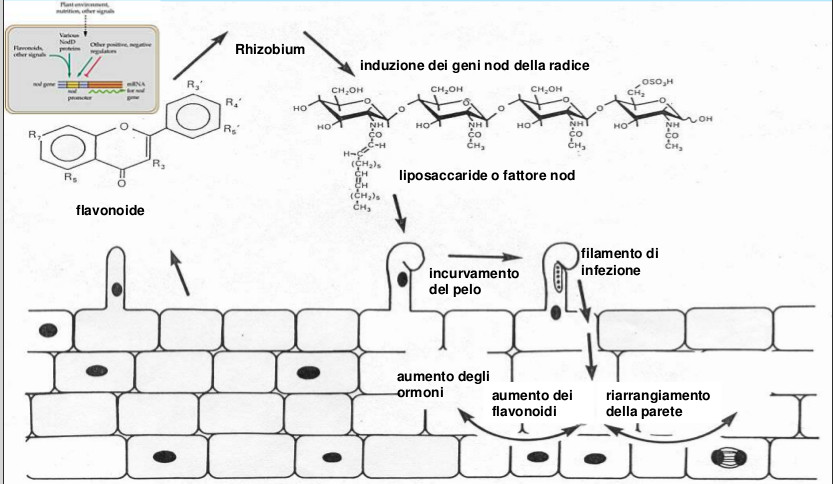
\includegraphics[scale=0.35]{immagini/leguminose.jpg}
\caption{Comunicazione tra pianta e batterio}
\end{figure}

Inizia una via di segnalazione per preparare la pianta ad accogliere il batterio : inizia la formazione del nodulo.
I fattori NOD sono dei lipo-chito oligosaccaridi con scheletro di N-acetilglucosammina. La specificità per una certa pianta può essere più o meno elevata. Rimangono circoscritti alla zona prossima alla parete cellulare del batterio, e non diffondono ma devono venire a contatto con la parete cellulare del pelo radicale affichè siano sentiti dalla pianta. Sono i responsabili dell'inizio della proliferazione cellulare che porta alla forazione del nodulo; si osserva un aumento di flavonoidi all'interno della pianta.

È il fattore NOD che determina la curvatura del pelo radicale.

\subsection{La via comune di segnalazione SYM}
 Via comune perchè è comune sia alla risposta della pianta a batteri azotofissatori, sia alla simbiosi micorrizico-vescicolo apuscolare.
Queste vie si sviluppano in risposta alla percezione del NOD Factor: ci sono recettori chinasici, canali ionici (castor e polluce) che determinano, al momento della percezione di NOD, una variazione prolungata nel tempo dei livelli di calcio intracellulare.

È comune anche alla via di segnalazione in risposta ad agenti patogeni.

I geni NOD sono espressi su un plasmide, che contiene anche i geni per la nitrogenasi e un operone per la replicazione del plasmide.
Se questo plasmide si attiva al momento della simbiosi, d'altra parte nella pianta si ha riarangiamento della struttura genetica: nelle cellule non infettate, si ha maggior espressione di enzimi per assimilazione e fissazione dell'azoto; nelle cellule infettate c'è espressione dei geni delle noduline, tra cui geni per l'assimilazione dell'azoto e per la leg-emoglobina, per mandare l'ossigeno nel simbiosoma.

La risposta all'infezione da parte della pianta è diversa da quello che comporta la formazione del filamento di infezione: la pianta risponde con aumento delle divisioni nella regione del parenchima corticale.

In alcuni casi come nell'arachide la penetrazione dei batteri avviene da rotture dell'epidermide.

Una volta che i batteri sono stati riconosciuti e si è formato l'uncino, i batteri penetrano nel pelo radicale ma non entrano nel citopasma perchè esso si invagina e crea un filamento nel quale questi batteri si muovono, grazie all'apposizione di elevati frammenti di membrana per elevata produzione da parte del golgi della cellula pilifera stessa. Quando finisce, i batteri vanno nell'apoblasto, degradano la parete della cellula e raggiungono la zona in cui si trova il meristema primario del nodulo: la parete del batterio e la membrana plasmatica vengono perse e si istaura la \emph{membrana peribatteroidea}.

Il nodulo è vascolarizzato. I batteroidi arrivano al meristema primario tramite il filamento di infezione.

(10.11.14)

Nella simbiosi si attivano due programmi genetici: uno permette il riconoscimento del batterio da parte della pianta e la penetrazione dentro la pianta, con formazione del \emph{filamento di infezione}, l'altro porta all'attivazione di due zone meristematiche, il meristema primario del nodulo e quello secondario, che si accrescono in direzione della zona di penetrazione dei batteri. Si forma il nodulo maturo.
Alla periferia del nodulo c'è un tessuto vascolarizzato in connessione col fascio vascolare radicale. 

I batteroidi si trovano nella cellula in numero elevato e avvolti dalla membrana peribatteroidea. Il vacuolo è contratto perchè le cellule hanno subito un riarrangiamento strutturale per permettere la simbiosi.

\subsection{La fisiologia del nodulo}
Il nodulo mantiene un amibente in cui è scarsamente presente l'ossigeno. 

La parete del nodulo è quella che impedisce l'accesso dell'ossigeno; è rivestito da uno strato fibroso che a sua volta impedisce l'entrata dell'ossigeno.

L'ATP viene prodotto con la catena respiratoria, utilizzando gli elettroni provenienti dall'ossigeno: di fatto quindi l'ossigeno serve \lfreccia sistema di captazione dell'ossigeno anche ai bassi livelli che ci sono nel nodulo, grazie ad una proteina codificata dai geni della pianta, la \textbf{leghemoglobina}, che ha altissima affinità per l'$O_2$: lo lega alla periferia della cellula. Lo spostamento della leghemoglobina avviene per gradiente di concentrazione: è più concentrata alla periferia della cellula e meno al centro della cellula. L'ossigeno viene impiegato da un sistema metabolico che sfrutta una citocromo ossidasi, che ha elevata affinità per l'$O_2$, e che permette il mantenimento della catena di trasporto degli elettroni \lfreccia mantenimento di ATP.

La corrente floematica porta al batterio i prodotti della fotosintesi.
(vedi la slide "Biochimica e fisiologia del nodulo").
Il batteroide riceve C dal malato, e questo produce anche equivalenti riducenti, che servono per attivare la catena respiratoria e per ridurre l'attività della nitrogenasi reduttasi (proteina 2), che viene ridotta dalla ferridossina ridotta prodotta attraverso l'ossidazione del malato (proprio con quegli equivalenti riducenti).
L'ammonio prodotto dal batteroide viene esportato nella cellula vegetale, che contiene la glutammina sintetasi \lfreccia Asn e Glu, ma anche allantoina ed acido allantoico. 
La cellula vegetale organica l'ammonio e viene esportato al resto della pianta attraverso lo xilema; se è in eccesso, viene trasferito al batteroide per l'accrescimento del nodulo. 

Le piante tropicali non devono fissare una quantità elevata di C per fissare l'azoto, perchè contengono le ureidi, che hanno un alto rapporto N/C.

\subsection{Bilancio energetico dell'azotofissazione}
16 ATP per 1 $N_{2}$, alle quali si aggiungono 9 ATP necessari per la produzione del potere riducente da incorporare nella ferridossina per rigenerare l'attività della nitrogenasi redutassi \lfreccia 25 ATP per 1 $N_{2}$.

Per l'assimilazione di $N_{2}$ da $NO_{3}$, per assimilare 1 $NO_{3}$ servono 12 ATP. Poichè la pianta riceve energia dal processo fotosintetico, esiste una stretta coordinazione in termini di C organicato e di potere riducente che la pianta rende disponibile (prodotto anch'esso dal processo fotosintetico) \lfreccia \textbf{fotoassimilazione} proprio per questa stretta coordinazione tra fotosintesi e assimilazione di $N_{2}$.

Se la pianta ha soddisfatto le esigenze di C, allora procedono le altre assimilazioni.

\chapter{La fotosintesi}
Processo che converte l'energia solare (fotoni) in energia chimica (legame, ATP, NADPH), per l'\emph{organicazione del carbonio}. Viene incorporata nella materia organica la $CO_{2}$. L'energia solare è usata dalla pianta per ossidare l'acqua, con la conseguente liberazione di ossigeno, e per ridurre il biossido di carbonio in composti organici, principalmente zuccheri.

\begin{equation}
\ce{6 $CO_{2}$ + 6 H2O -> C6H12O6 + 6 $O_{2}$}
\end{equation}

Questo processo richede $NADP_{+}$ e ADP e Pi. Il glucosio è un prodotto che porta all'accumulo sotto forma di amido se è in eccesso, altrimenti viene trasportato nella pianta come saccarosio.

La fotosintesi avviene in tutte le piante, procarioti (alghe azzurre, ecc) ed eucarioti. A seconda dei pigmenti, il colore delle piante/batteri/alghe/cambia.

Il numero di cloroplasti può essere aumentato per aumentare la capacità di captazione della luce: il \emph{cloroplasto} infatti contiene pigmenti per la captazione della luce. I cloroplasti stanno in tutti i tessuti verdi delle piante. Hanno un'anatomia e un'istologia tale da favorire il più possibile l'attività fotosintetica: mesofillo a palizzata rivolto verso la parte superiore della pianta, le cui cellule conengono i cloroplasti; sotto cellule del parenchima spugnoso, a livello del quale avvengono gli scambi gassosi.
\begin{figure}[H]
\centering
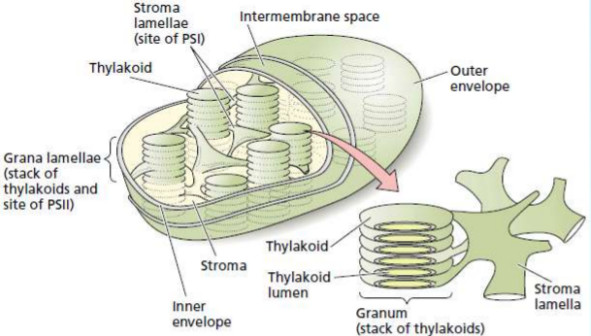
\includegraphics[scale=0.35]{immagini/cloroplasto.jpg}
\caption{Anatomia del cloroplasto}
\end{figure}

Il lato inferiore è 5 micron e il maggiore 45-50 micron; doppio set di membrana, una esterna che fa da rivestimento per l'organulo e una interna che si ripiega verso lo stroma, formando strutture vescicolari (tilacoidi) apiattite che in alcuni casi si impilano fra loro (grana) e sono collegati dalle lamelle intergrana. Nelle vescicole è presente un lumen.

La membrana tilacoidale è costituita da glicolipidi e galattolipidi, e molecole apolari come colesteroli e chinoni, oltre a pigmenti (clorofille e carotenoidi) e i complessi fotosistema I e fotosistema II, che convertono l'energia luminosa in energia chimica, e molecole che fanno parte della catena luminosa tra i due fotosistemi; è attraverso la membrana tilacoidale che i protoni entrano nello stroma, vanno nel lume e verranno usati per produrre ATP. All'interno dello stroma vengono rilasciati prodotti della fase luminosa della fotosintesi, quali l'ATP (rilasciato dall'ATPsintasi) e il NADPH.

La strutturazione del cloroplasto è finalizzata alla chimica e alla fotochimica della fotosintesi.

\paragraph{Genoma del cloroplasto}
DNA circolare aquisito tramite endosimbiosi con un procariote. Alto grado di conservazione dei cromosomi.
Ci sono proteine tipiche del cloroplasto che sono codificate parzialmente dal genoma della pianta e del cloroplasto stesso, ad esempio la subunità grande della RuBisCO. La funzionalità del cloroplasto è strettamente dipendente dalla funzionalità della cellula che lo ospita.
\paragraph{}
I cloroplasti nelle foglie senescenti vengono recuperati per essere distribuiti nelle foglie giovani \lfreccia da ciò derivano le colorazioni autunnali, ovvero dalla rimozione della clorofilla dal cloroplasto, che lascia vedere gli altri pigmenti presenti nella foglia, i \emph{carotenoiodi}, normalmente oscurati dalla clorofilla.

La comprensione della capacità di organicare il carbonio è piuttosto recente; prima si riteneva che la pianta mangiasse il suolo con le radici. 
Hill nel 1939 scoprì che i cloroplasti erano grado di ossidare l'acqua, essendo il ferro l'accettore di elettroni, formando $O_{2}$. Descrive la fotosintesi come un processo di ossidazione dell'acqua in cui gli elettroni vengono trasferiti al ferro.

L’evento primario della fotosintesi è un’ossidazione e gli elettroni sono trasferiti
dall’acqua ad un altro composto (conversione dell’energia luminosa in energia
chimica); l’accettore naturale di elettroni a quel tempo era ancora sconosciuto.
Il processo fotosintetico è responsabile della produzione di tutto
l’ossigeno atmosferico e della fissazione di circa 1011 tonnellate per
anno di C dalla $CO_{2}$ in composti organici.

Fotosintesi e respirazione sono processi opposti.

Le reazioni al buio possono avvenire solo se sono avvenute le reazioni alla luce, prechè ne impiegano i prodotti. 
Le reazioni alla luce sono mediate dall'energia luminosa, captata dalla clorofilla, e attraverso i fotosistemi portano a sintesi di ATP, NADPH e $O_{2}$; le reazioni al buio portano all'incorporazione di $CO_{2}$ nei triosi fosfati, grazie a NADPH, che portano alla sinetesi degli esosi fosfati.

(17.11.2014)

Accumulo di protoni nel lume e nel lato interno della membrana tilaciodale; serviranno per la produzione di ATP.
Tutte le reazioni "alla luce" portano all riduzione del $NADP^{+}$+.

Le lunghezze d'onda dello spettro della radiazione solare vanno da lunghe ad inferiori e parallelamente alla riduzione della lunghezza aumenta la frequenza.

Spettro del visibile: 400(blu) -700 (rossa)nm.

L’energia recata da un fotone dipende da  $E=\lambda \ni = \frac{h c}{\lambda}$.

A basse lunghezze d’onda corrispondono alti livelli di energia. La luce blu ha più efficienza in termini di fotosintesi della luce rossa.

\paragraph{Irradianza}

La quantità di energia che in un dato momento colpisce una data superficie. Viene espressa in termini di \emph{calore} , di \emph{$W/m^{2}$} o di \emph{moli di fotoni $m^{-2}$ $s^{-1}$}.

Le piante impiegano per la fotosintesi solo alcune lunghezze d’onda. Lo spettro della luce solare è composto  in particolare di 5\% di UV (<400 nm), il 28\% del visibile e il 67\% dell’infrarosso (<740 nm).

Tale distribuzione viene modificata dal passaggio dell’energia solare attraverso l’atmosfera: l’infrarosso viene parialmente assorbito dallo strato d’ozono e la sua intensità viene assottigliata \lfreccia la pianta la percepisce assottigliata.

Nell’atmosfera si ha un arricchimento della radiazione visible: dal 28\% si arriva al 45\%, con parallela riduzione delle componenti UV ed infrarosse.

\textbf{PAR}: radiazione fotosinteticamente attiva, ovvero le lunghezze d’onda che permettono alla fotosintesi di funzionare.

\paragraph{Pigmenti fotosintetici}

Capacità di assorbire luce nel range del visibile, e proprio per questo si rendono visibile all’occhio umano.

\begin{itemize}

\item{Clorofille: in tutti gli organismi fotosintetici, sono a livello dei sistemi antenna che percepiscono grandi quantità di luce,  e nel centro di reazione}

\item{Carotenoidi: pigmenti accessori perchè coadiuvano la clorofilla nella ercezione della radiazione luminosa. Sono in grado di assorbire luce a unghezze d’onda diverse, e riescono a conferire l’energia assorbita alla clorofilla stessa}

\item{Biliproteine o ficobiline: presenti in alghe rosse e cianobatteri. Sono proteine che legano un cromoforo. Possono essere associati a proteine}

\end{itemize}

Le clorofille sono verdi perchè assorbono a certe lunghezze d’onda. Si trovano a livello dei grana, immerse nello strato lipidico.

Le principali sono le \emph{clorofille a}: possoo subire modificazioni sull’anello pentapirrolico. La testa è la porfirina alla quale è lagata la coda di fitolo attraverso l’acido propionico.(supercazzola) Presenta uno ione $Mg^{2+}$ che delocalizza le cariche condividendole con gli atomi di azoto con cui si coordina \lfreccia la clorofilla non è una molecola carica. Assorbe a 450 nm.

La clorofilla B presenta un gruppo metile sostituito, per il resto è uguale alle a. Non è presente in tutti gli organismi come la a, ma sicuramente è nelle alghe e nelle piante superiori come la clorofilla c. Assorbe a 480 nm.

La feofitina è una clorofilla che non presenta lo ione Mg; la clorofillide invece non ha la coda di fitolo.

\paragraph{Lo spettro di assorbimento delle clorofille}

La clorofilla assorbe con due massimi nel blu e nel rosso, non assorbe nel verde ( e per questo è verde, perchè la riflette).

\section{Carotenoidi}

I carotenodi sono lipidi con 40 C  sono dividi in due classi a seconda che presentino o meno ossigeno nelle strutture: rispettivamente Xantofille e Caroteni. Sono pigmenti accessori.

Hanno due picchi e una spalla di assorbimento, e compensano ad alti livelli di energia la capacità di captazione delle clorofille.

\paragraph{Caroteni}

Derivano dalla via dei tetraterpeni. Una volta che lo scheletro a 40 C è stato prodotto, la va biosintetica prende origine a partire dal Licopene, e da qui si originano Caroteni e xantofille.

Utilizzati per la percezione della radiazione solare perchè fnano parte del sistema antenna.

\paragraph{Xantofille}

Forti antiossidanti, utilizzate per proteggere il fotosistema dalla fotossidazione. Sono ossigenate (vedi luteina, la principale xantofilla). anche Zeaxantina, Violaxantina per l’apertura stomatica.

Funzioni dei carotenoidi: espandere lo spettro di assorbimento per la fotosintesi; proteggere il sistema dalla fotossidazione. La luce eccita i pigmenti, gli elettroni si muovono fino a che il ciclo di Calvin rallenta: abbiamo ora un accumulo di NADPH e composti ridotti, e non c’è più accettore di elettroni, quindi spesso si usa l’ossigeno. Le xantofille impediscono ciò.

In vivo le interazioni dei pigmenti con l’ambiente fa si che i livelli di energia necessari per l’eccitazione dei pigmenti cambino.  Lo spettro funzionale alla fotosintesi viene definito \emph{spettro d’azione}: mette in relazione la capacità di assorbimento a diverse lunghezze d’onda con la capacità fotosintetica (misurata tramite la quantità di ossigeno prodotto).  Lo spettro di assorbimento e di azione coincidono quasi perfettamente.

Quando un pigmento assorbe luce, l’energia ricavata dal decadimento di un elettrone viene convogliata al centro di reazione, mentre parte viene persa.

Le radiazioni comprese nel visibile sono in grado di dare eccitazione dei pigmenti: questo perchè sono presenti doppi legami coniugati \lfreccia più ce ne sono, meno energia serve per eccitare un elettrone ad un livello superiore. Sono necessari almeno 7 legami coniugati per i pigmenti per essere tali.

I livelli energetici assorbiti dai pigmenti sono 300 Kj/mole per i fotoni blu  e 160 Kj/mole per un fotone nel rosso.

La luce blu contiene energia che non permette di produrre una reazione fotosintetica più energizzata rispetto alla luce rossa. Quindi è prevalentemente quella rossa impiegata nella fotosintesi.

L’energia assorbita può essere rilasciata come calore o come luce (fluoresenza o fosforescenza - quando lo stato di triplette eccitato torna a livello basale).

Un’altra modalità conivolge le molecole del complesso antenna e si ha per trasferimento dell’energia ad alte molecole: un pigmento del sistema antenna torna allo stato basale. Si riesce così a catturare livelli energetici via via decrescenti perchè man a mano che il trasferimento avviene, si ha comunque una perdita in calore.

L’ultimo modo è attraverso la fotochimica: mentre tutti i pigmenti non perdono elettroni, nel centro di reazione, molecola dimerica, si ha perdita di elettroni.

(24.10.2014)

Anche il decadimento è un evento rapido.

\section{De-eccitazione dei pigmenti}
\paragraph{Decadimento non radiante}
La molecola torna allo stato fondamentale o ad uno stato eccitato inferiore tramite il rilascio
dell’energia come calore.
Il tempo necessario per decadere allo stato fondamentale o ad uno stato eccitato inferiore è circa
$10^{-12}$ s.

Quando la clorofilla A eccitata da un fotone del blu fa tornare il singoletto eccitato allo stato precedente.
\paragraph{Decadimento radiante}
può avvenire per \emph{fluorescenza} o per \emph{fosforescenza}.

\textbf{Fluorescenza}: emissione di luce in circa $10^{-9}$ s; dal primo stato di singoletto eccitato la
molecola torna allo stato fondamentale, per cui la clorofilla eccitata deeccita per emissione di fluorescenza.
Il salto energetico che separa fotone nel blu e nel rosso, viene perso sotto forma di calore per decadimento non radiattivo. Il fotone blu invece è molto efficace per la fotosintesi, ma a seconda delle condizioni questa energia può essere persa come fluorescenza nel rosso (contenuto energetico inferiore rispetto al fotone eccitante ma $\lambda$ maggiore). Se irraggiamo clorofilla in soluzione con luce nel blu, si ha emissione di fluorescenza nel rosso: la clorofilla in soluzione è in un ambiente molto diverso rispetto al cloroplasto (e il decadimento avviene in maniera diversa). La fluorescenza è di fatto un fenomeno di decadimento molto raro nella foglia, perchè nella foglia la clorofilla è legata a complessi proteici.

\textbf{Fosforescenza}: emissione di luce molto lenta (tra $10^{-3}$ e 10 s). Si verifica quando le molecole,
dallo stato di tripletto tornano allo stato fondamentale.

\paragraph{Risonanza} nel sistema di pigmenti organizzati avviene frequentemente un trasferimento di energia per \emph{risonanza}: attraverso movimenti vibrazionali, la vibrazione dell'elettrone eccitato viene trasferita ad una molecola nel pigmento adiacente (distante max $10 nm$). L'energia trasferita è comunque minore di quella che ha il tripletto che trasferisce \lfreccia l'ultima molecola è quella che assorbe meno di tutte ed è quella che realizza la reazione fotochimica \lfreccia \emph{Unidirezionalità} del trasferimento di energia.

\paragraph{Reazioni fotochimiche} soltanto poche molecole di clorofilla possiedono questo meccanismo di de-eccitazione: le clorofille “trappola” dei centri di reazione P680 e P700.
Questa molecola perderà un elettrone, che verrà trasferito ad un accettore primario, la molecola del centro di reazione (dimero di clorofilla A): questa converte l'energia della radiazione luminosa in energia chimica.

Nella fotossidaizone la clorofilla, eccitata dall'ultimo pigmento che porta la luce del fotone, viene ossidata: si forma il radicale cationico e l'elettrone viene ceduto all'accettore primario, la porfirina (o plastocianina - fotosistema 1).
\paragraph{}
La maggior parte dell'energia solare che colpisce i pigmenti porta al processo fotochimico.

\section{Pigmenti e proteine che costituiscono il fotosistema}
Distinguiamo 2 componenti del fotosistema:
\begin{itemize}
\item{Complesso antenna}
\item{Centro di reazione: complesso tra proteine e pigmenti. }
\end{itemize}
Questo fotosistema è in grado di portare avanti una parte del processo della fotosintesi

A livello dell'antenna ci sono moltissimi pigmenti e proteine: ciò garantisce un \emph{alto livello di eccitazione della clorofilla}, poichè la loro funzione è assorbire la luce. Il centro di reazione è formato da proteine,
pigmenti e trasportatori di elettroni e contiene una speciale molecola di \emph{clorofilla a} (P) che converte
l’energia luminosa in energia chimica. 
\begin{figure}[H]
\centering
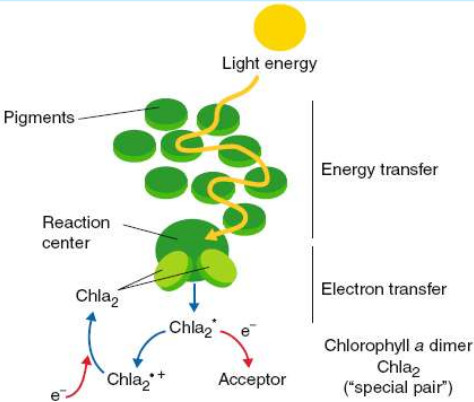
\includegraphics[scale=0.35]{immagini/antenna.jpg}
\caption{Trasferimento di energia nel complesso antenna}
\end{figure}
Trasferimento di energia nel complesso antenna: l’energia della luce è
assorbita dai pigmenti dell’antenna e trasferita a molecole adiacenti,
finchè raggiunge due particolari molecole di clorofilla nel centro di
reazione. Il dimero di \emph{Chl a} emette un elettrone verso un accettore,
diventando un radicale carico positivamente, che è quindi in grado di ricevere elettroni da altre molecole. Questo torna allo stato
fondamentale acquistando un elettrone, che proviene dalla fotolisi dell'acqua.


\section{Fotosistemi I e II}
Per ogni molecola di $O_2$ rilasciato si avevano 2500 molecole di Chl (clorofilla).

La luce blu viene persa sotto forma di calore nella deeccitazione da secondo singoletto eccitato a primo singoletto eccitato. Al di sopra di determinate $\lambda$ l'efficienza fotosintetica cade bruscamente (\emph{Red Drop}).

Irradiazione contemporanea con 2 diverse lunghezze d'onda produce una velocità di fotosintesi maggiore di quella che si avrebbe sommando le velocità ottenute irradiando separatamente con le due diverse $\lambda$. Si concluse che esistono 2 fotosistemi che lavorano insieme. Questo si chiama \emph{effetto di amplificazione}.

Esistono 2 fotosistemi che hanno al centro due molecole di clorofilla che assorbono a 700 nm (P700) nel fotosistema I e a 680 nm (P680) nel fotosistema II.

Si trovano nella mebrana che separa lume e stroma, hanno una distribuzione particolare ed un orientamento particolare:
\begin{itemize}
\item{PSII : localizzato nelle \emph{lamelle dei grana} insieme alle sue clorofille antenna e alle proteine di trasporto elettronico}
\item{PSI : nelle \emph{lamelle stromatiche} principalmente\footnote{Anche sui bordi delle lamelle dei grana}, insieme ai pigmenti, alle proteine di trasporto elettronico, come l'ATPasi}
\end{itemize}

Il citocromo \emph{$b_{6}$f}, che fa parte della catena di trasporto elettronica che unisce i due fotosistemi, si trova equamente distribuito fra le lamelle stromatiche e quelle granali.
C'è un complesso CORE centrale che contiene la clorofilla e un sistema antenna intorno.

La distribuzione dei pigmenti è in prevalenza clorofille: su 600 molecole di clorofille, 450 sono A e 150 B. La maggior parte della A si trova nei complessi antenna, solo il 40\% si trova nel centro di reazione.
La clorofilla B sta solo nei complessi antenna, come i carotenoidi.

I fotosistemi 2 prevalgono in termini numerici rispetto all'1.

La luce arriva nei pressi dei carotenoidi, i quali trasferiscono l'energia alla clorofilla B e poi alla A, fino al centro di reazione (si va verso livelli energetici via via inferiori).

La molecola del centro di reazione, quando ha ricevuto energia dai pigmenti adiacenti, non la può cedere di nuovo per risonanza: non può tornare indietro perchè non è sufficente ad eccitare le molecole adiacenti. Per de-eccitarsi quindi o fluorescenza o perdita diretta dell'elettrone. 
La struttura del centro di reazione è tale da favorire questo rilascio, poichè c'è una molecola che accetta l'elettrone perso dalla P680 o dalla P700. L'elettrone verrà poi rispristinato da un donatore, che è l'acqua. 

La P680 perde un elettrone ed assorbe luce: diventa così in grado di strappare uno alla volta elettroni all'acqua (diventa un riducente): può così trasferire elettroni secondo gradiente di potenziale redox alla P700, che a sua volta ha perso elettroni (ossidante); assorbendo un fotone la P700 viene ossidata ed è diventata un forte riducente e riesce a trasferire un elettrone alla ferridossina che a sua volta lo trasferisce al $NADP^{+}$ riducendolo a NADPH. (vedi Schema Z sulle slides). 

Questi complessi proteina-pigmento, avendo una determinata posizione ed orientamento, permettono l'accumulo di protoni nel lume \lfreccia gradiente che viene sfruttato dall'ATPsintasi. 

Il PSII perde elettrone e lo trasferisce, ma lo ripristina strappandolo all'acqua. Dal PSII l'elettrone viene trasferito al plastochinone e poi al citocromo \emph{$b_{6}$f}. La plastocianina lo trasferisce al PSI e qui va a ridurre la ferridossina che ridurrà il $NADP^{+}$ a NADPH.

La localizzazione precisa dei fotosistemi è essenziale: il PSII si trova principalmente nelle zone appressate dei grana, il PSI nelle zone non appressate e in quelle che guardano verso lo stroma. Il sistema citocromico si trova dislocato fra le due zone. L'ATP sintetasi si trova in entrambe le zone.

Il complesso antenna può dissociarsi per evitare eccessivi livelli di captazione dell'energia luminosa.

\subsection{Fotosistema II}
Qui si realizza la reazione:

\begin{equation}
\ce{2 PQ + 2 H2O -> $O_{2}$ + 2 PQH2}
\end{equation}


Il complesso proteico che realizza la reazione di fotolisi deell'acqua si trova nella parte de lumen (OEC).

Il complesso \emph{core} è dato dalle proteine D1 e D2 che legano non solo P680 ma anche i trasportatori che portano gli elettroni al chinone. Troviamo la clorofilla nel centro di reazione, un dimero di 2 clorofille A: ciascuna lega una molecola di feofitina (Chl priva di Mg) e due chinoni, Qa(associato a D2, riceve per primo gli elettroni ed è immobile) e Qb(associato a D1, è mobile e riceve l'elettrone da Qa), che ricevono elettroni dalla feofitina. Il residuo di tirosina che si trova affacciato sul lato luminale e fa parte della proteina D1, trasferirà l'elettrone dagli atomi di Mn dell'OEC alla clorofilla. L'acqua trasferisce gli elettroni al Mn rimpiazzando l'elettrone perso dalla clorofilla (che è finito al citocromo B6F).

Il centro di reazione di PSII cederà poi elettroni alla feofitina.

\paragraph{Complesso antenna associato (LHC II)}
 
È formato da proteine e pigmenti legati da interazioni deboli al core complex.  È costituito da un antenna principale, i polipeptidi CP43 e CP47 associati a D1/D2 e ad un numero variabile di molecole di clorofilla - circa 20/25. Questi polipeptidi sono codificati dal genoma cloroplastico. 

C'è anche un'antenna periferica che ha struttura trimerica: porta un polipeptide che porta Chl a, Chl b e carotenoidi \lfreccia sistema antenna centrale.

CP indica che i polipeptidi sono codificati dal genoma cloroplastico.

(1.12.2014)
\paragraph{}
A livello del fotosistema II si realizza la fotolisi dell'acqua. P680, una volta eccitato, diviene un debole riducente e riesce a trasferire il proprio elettrone alla catena di trasporto degli elettroni, diventando così un forte ossidante e riuscendo a strappare elettroni all'acqua. Affinchè si abbia la riduzione dell'acqua devono essere persi da P680 4 protoni.

Il fatto che i fotosistemi e la catena di trasporto degli elettroni abbiano una localizzazione ben definita nella membrana tilacoidale fa si che si realizzi una vera e propria separazione di carica: si evita il ciclo futile, ovvero il ritorno dell'elettrone perso dal P680 al P680 stesso. Così P680 deve trovare un'altra fonte di elettroni (l'acqua) per tornare allo stato iniziale di forte ossidante. 

\subsection{Ossidazione fotosintetica dell'acqua}
Il \emph{complesso OEC} (complesso di evoluzione dell'ossigeno) è associato al fotosistema II e permette la realizzazione della reazione di \emph{fotolisi dell'acqua}, fornendo elettroni al P680 ossidato. 4 protoni consecutivamente staccano 4 elettroni che vengnono prelevati da 2 molecole di acqua. Questo complesso è costituito da un numero variabile di catene tra cui la proteina MSP33 che contiene un cluster di Mn e del Ca. Il Ca stabilizza il cluster di Mn. Questa proteina stabilizza nell'ambiente il complesso dei 4 atomi di Mn. (vedi slides)

Non sappiamo bene come la fotolisi dell'acqua sia mediata dal Mn. La P680 eccitata da 4 fotoni successivi si trova per 4 volte consecutivamente priva del suo elettrone: lo riceve dalla Tyr della proteina D1 che a sua volta li riceve dal cluster di Mn, il quale li preleva dall'acqua (non si sa come li preleva: sappiamo solo il processo complessivo, cioè che 4 atomi di Mn passano dallo stato fondamentale s0 a s1, s2, s3, s4). Gli elettroni vengono strappati tutti insieme da 2 molecole di acqua, producendo ossigeno e protoni: gli atomi di Mn tornano allo stato s0. Il fatto che gli elettroni vengono persi tutti insieme dall'acqua ci assicura che non si formino radicali anionici che sono tossici.

Il chinone B associato alla proteina D1 viene ridotto perchè ha ricevuto l'elettrone dal chinone A attraverso il Fe: l'elettrone deve essere trasferito lungo la membrana tilacoidale per sostituire quello perso dalla P680. Il plastochinone si viene a trovare in forma radicalica: riceve un secondo elettrone da $Q_{A}$ e prelevando 2 H+ dallo stroma diventa $QH_{2}$. Si spostano quindi 2 elettroni alla volta.

\paragraph{Citocromo b6F}
È costituito da una proteina Fe-S di Rieske, 2 citocromi b6 e un citocromo f. È presente un polipeptide 4 la cui funzione è sconosciuta. Queste catene polipeptidiche sono trasnmembrana e ricevono gli elettroni dal plastochinone.

Il trasferimento di elettroni si completa in un ciclo che trasferisce 2 elettroni al citocromo b6F. Si realizza il \emph{ciclo dei chinoni} che porta i 2 elettroni alla plastocianina , ma allo stesso tempo vengono traslocati nel tilacoide 4 protoni. Questi due elettroni vengono trasferiti uno alla volta al PSI: uno viene trasferito al cit b che lo trasferisce ad un plastoidrochinone $QH_{2}$.

$QH_{2}$ cede il primo elettrone al Rieske e questo lo cede al citocromo f e quindi alla plastocianina (PC) che, diffondendo nel lume, giunge al PSI. Il secondo elettrone di $QH_{2}$ è ceduto al citocromo b che lo cede ad una molecola di plastochinone ossidato, che diventa Q-. I 2 protoni trasportati da QH2 sono immessi nel lume.
\begin{figure}[H]
\centering
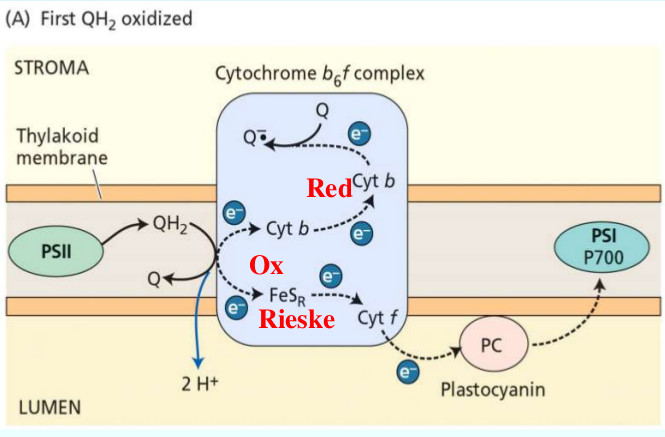
\includegraphics[scale=0.35]{immagini/chinone.jpg}
\caption{Ciclo dei chinoni}
\end{figure}
A questo livello, per ogni 2 $e^{-}$ traslocati alla plastocianina vengono rilasciati nel lume $4 H^{+}$. Questo è fondamentale per generare la differenza di concentrazione protonica ai due lati della membrana, utile per la sintesi di ATP. Esiste quindi un pool di chinoni ridotti e ossidati lungo la membrana tilacoidale: la presenza di chinoni ossidati nello stroma del cloroplasto permette l'esistenza del ciclo dei chinoni.

\paragraph{Plastocianina} 
(PC) è una proteina solubile con massa 11 KDa localizzata nel lume. Trasporta elettroni dal complesso
citocromico b6f al P700. Il centro redox è uno ione rame ($Cu^{2+}$) legato allo S delle catene laterali di una cisteina (Cys 84) e di una metionina (Met 92) e allo N di due istidine (His 37 e His 57). Nella forma ossidata la plastocianina è blu. Il rame accetta un elettrone passando a Cu+. La plastocianina ha una struttura cristallina a barile ($\beta$–barrel). In generale la struttura a barile è costituita da foglietti $\beta$ che si intrecciano e si avvolgono originando una struttura chiusa in cui il primo
filamento è legato con legame ad H all’ultimo. La struttura a barile si ritrova anche nelle porine.

Solubile e mobile, fa da shuttle elettronico. L'atomo di Cu riceve elettroni dal citocromo b6F perchè la plastocianina si trova legata tramite legami elettrostatici a livello della catena polipeptidica del \emph{citocromo f} sul lato luminale. Al momento in cui viene ridotta si sposta nel lume del tilacoide e va ad interagire con PSI, cedendo l'elettrone alla P700.
\paragraph{}
 In conclusione: 4 H+ sono immessi nel lume ogni 2 elettroni trasportati dalla Plastocianina al P700 e ciò porta ad un aumento di
protoni nel lume rispetto a quello che sarebbe stato ottenuto con il trasporto lineare (Rieske, citocromo f, plastocianina,
PSI), cioè 2 H+ immessi nel lume ogni 2 elettroni trasportati dalla PC al P700.
   
\section{Fotosistema I}
In questo fotosistema non si distingue un complesso core da uno antenna periferico: i pigmenti antenna rivestono il centro di reazione.
\begin{figure}[H]
\centering
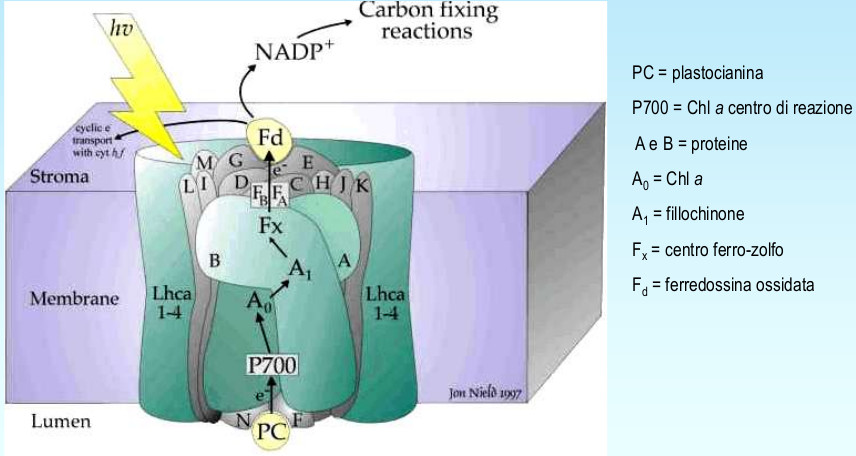
\includegraphics[scale=0.35]{immagini/PSI.jpg}
\caption{Struttura del PSI}
\end{figure}

Ci sono le catene A e B, omologhe alle proteina D1 e D2. Vi troviamo il centro di reazione P700, costituito da un dimero di clorofilla a, un fillochinone e un centro Fe-S che riceve elettroni dal fillochinone. Essi vengono poi trasferiti alla ferridossina ossidata e questa li trasferisce al $NADP^{+}$ che diventa NADPH.
\begin{figure}[H]
\centering
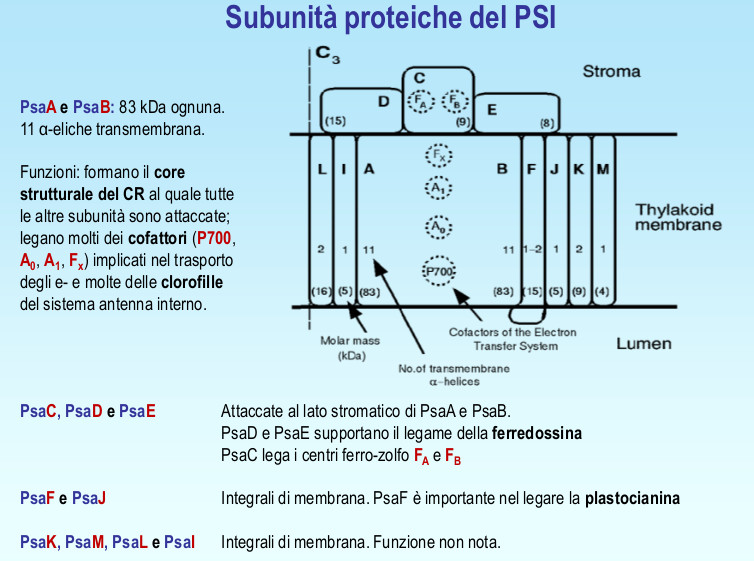
\includegraphics[scale=0.4]{immagini/proteine.jpg}
\caption{Subunità proteiche del PSI}
\end{figure}
Presenta due porzioni che associano la plastocianina (lato luminale) e la ferridossina (lato stromale).

La ferridossina è legata sul lato stromatico tramite i polipeptidi D ed E.
Il donatore primario di elettroni è il P700, costituito da un
dimero di Chl a di cui una sola molecola si fotoossida:

Fotoni \lfreccia chl* \lfreccia $chl^{+}$ + e-.

Associato al P700 vi è una chl monomerica detta $A_{0}$
che agisce come accettore immediato, vi sono poi 2
molecole di fillochinone $A_{1}$.

\subsection{Trasporto elettronico}
Le proteine A e B coordinano il trasferimento elettronico dalla plastocianina al centro Fe-S compreso tra le due subinità; la subunità F è coinvolta nel legame con la plastocianina perchè ha una componente nel tilacoide.
La subunità C riceve elettroni dai centri Fe-S del \emph{complesso core}. 

La ferridossina ridotta cede l'elettrone al $NADP^{+}$ che diventa NADPH e si forma ferridossina ossidata.
La luce rossa lontana (>680 nm) assorbita dal PSI causa l’ossidazione del centro di reazione (P700) e la
produzione di un forte agente riducente (P700* eccitato) che cederà un elettrone, tramite la ferredossina, al $NADP^{}$
(in totale 2 e- in due cicli successivi). A seguito della reazione di ossidazione il P700 si trasforma in un debole 
agente ossidante (P700+) che recupera l’elettrone perso dalla plastocianina.

L'enzima \emph{ferridossina NADP+ reduttasi} catalizza la reazione. La ferridossina è associata alle subunità D ed E del fotosistema I con legami elettrostatici: al momento in cui si riduce si stacca e diventa substrato di questo enzima.
I protoni che servono per sintetizzare $NADPH_{2}$ vengono presi dallo stroma.

\section{Regolazione dell'assorbimento della luce}

In risposta ai diversi livelli di irradianza possono cambiare i rapporti stechiometrici tra i componenti del tilacoide in modo da:
\begin{itemize}
\item{Regolare la quantità di energia solare assorbita in relazione alla capacità di utilizzo da parte della pianta}
\item{Equilibrare i flussi di energia tra i fotosistemi (i fotosistemi non sono normalmente in rapporto stechiometrico 1:1!)}
\item{Prevenire la fotoinibizione}
\end{itemize}

Se la sintesi dei carboidrati non procede in modo tale da utilizzare NADPH, il fotosistema I stalla , e quindi stalla anche il fotosistema II.

Il 2 ha il 33 \% in più di capacità di assorbire la luce rispetto al fotosistema I.

Come rispondono le piante ai vari livelli di irradianza?
\begin{enumerate}
\item{Adattamenti a lungo termine: piante che vivono in ombra o in piena luce. Per le piante in ombra si osserva un aumentato contenuto in termini di sistema antenna di PSII; presentano anche un numero più elevato di zone appressate dei grana (dove si concentra PSII). Per le piante in piena luce, si ha una ridotta estensione del sistema antenna di PSII ed aumento dei complessi a valle del PSII}
\item{Adattamenti a breve termine . Una risposta breve prevede come segnale di alta irradianza il plastoidrochinone ridotto: quando PSI non è in grado di funzionare con la stessa rapidità del PSII si ha un accumulo del plastoidrochinone \lfreccia si attivano una chinasi LHCII ed una fosfatasi: la chinasi fosforila il complesso antenna del PSII, determinandone la dissociazione: questo diffonde nelle regioni non appressate dei grana fino a PSI, con cui si associa, permettendo di impiegare gli elettroni in più del PSII.  Tale aumentato assorbimento di energia di PSI determinerà l’ossidazione di $PQH_{2}$. Quando i livelli di plastochinone tornano normali, la fosfatasi LHCII-P defosforila il complesso antenna e questo torna al PSII}
\end{enumerate}

\subsection{Il trasporto ciclico}
Il trasporto ciclico di elettroni coinvolge solo PSI. Gli elettroni passano al plastochinone (PQ) attraverso l’enzima
\emph{ferredossina-plastochinone ossido-riduttasi (FPQR)}. Esso ossida la ferredossina e riduce contemporaneamente il PQ. Si ha quindi un' ulteriore sintesi di plastochinone ridotto che permette la realizzazione del ciclo dei chinoni.

Tale trasporto determina la formazione di un gradiente protonico che servirà per la sintesi di ATP; non si formano però
né $NADPH_{2}$ né $O_{2}$.
\begin{figure}[H]
\centering
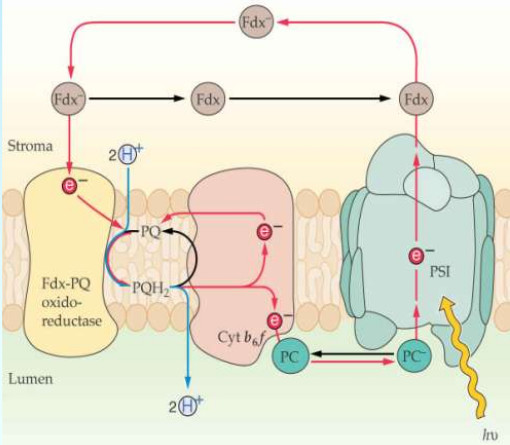
\includegraphics[scale=0.4]{immagini/ciclico.jpg}
\caption{Trasporto ciclico}
\end{figure}

Conclusioni: La ferridossina ridotta può quindi donare l’elettrone al NADP+ originando il trasporto non ciclico oppure donare l’elettrone al plastochinone via FPQR, dando luogo al trasporto ciclico.


\paragraph{Ruolo della ferridossina}
La ferridossina riduce un composto intermedio che presenta ponti disolfuro: attraverso essa segnala al ciclo di Calvin che ci sono abbastanza equivalenti riducenti per far funzionare il ciclo.

\section{Fotofosforilazione}
Sintesi di ATP attravero l'energia convertita da quella solare, quella non impiegata per la riduzione del $NADPS^{+}$ a NADPH. È resa possibile dal fatto che durante la catena di trasporto degli elettroni si crea una \emph{differenza di concentrazione protonica} ai due lati della membrana tilacoidale.

I protoni iniziano ad accumularsi già con la fotolisi dell'acqua; poi a livello del ciclo dei chinoni c'è un ulteriore rilascio di protoni nel lume del tilacoide; poi anche la sintesi di $NADH_{2}$ che preleva protoni. Questo gradiente protonico viene usato dall'ATP-sintetasi di membrana.
 
Jagendorf e Uribe (1966) isolarono tilacoidi granali da cloroplasti a pH 8, quindi trasferirono i tilacoidi
in una soluzione tampone a pH 4 equilibrandoli per 60 secondi. Successivamente trasferirono i
tilacoidi in un tampone a pH 8 e dopo un breve periodo aggiunsero ADP e 32Pi. Durante i
trasferimenti dei tilacoidi nei tamponi a diverso pH si genera un \emph{gradiente di pH} all’interno dei grana
(nel cloroplasto intatto il gradiente è prodotto dal trasporto elettronico tra i fotosistemi). In queste
condizioni si realizza la fosforilazione dell’ADP. L’esperimento, essendo effettuato al buio, dimostra
che la formazione di un gradiente elettrochimico protonico attraverso la membrana tilacoidale di
cloroplasti porta alla sintesi di ATP.

\begin{figure}[H]
\centering
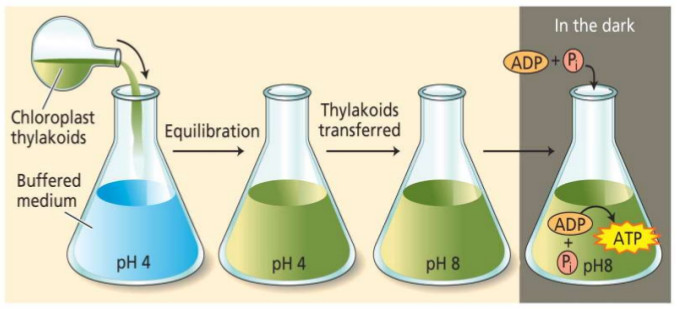
\includegraphics[scale=0.4]{immagini/chemiosmosi.jpg}
\caption{Ipotesi chemiosmostica alla base della fotofosforilazione}
\end{figure}

Pertanto l'energia per la sintesi di ATP nei cloroplasti ha origine dalla differenza di potenziale
elettrochimico degli H+ tra i due lati del tilacoide, causata dal movimento vettoriale di e-.

L’ATP sintasi converte in ATP l'energia del potenziale elettrochimico di membrana.
È stato proposto che l’energia totale disponibile per la sintesi di ATP o forza motrice protonica (proton
motive force = pmf espressa in mV) dipenda dal potenziale chimico dei protoni e dal potenziale elettrico
transmembrana. L’equazione seguente considera le due componenti:


\begin{equation}
\centering
\Delta P= \Delta E - 59 (pH_{i}-pH_{0})
\end{equation}

dove $\Delta E$ è la differenza di potenziale trasnmembrana e $pH_{i}$-$pH_{0}$ (o $\Delta$pH) è la differenza di pH attraverso la membrana. La costante di proporzionalità a 25\textcelsius è di 59 mV per unità di pH.

È il $\Delta$pH che guida la sintesi di ATP. 4 protoni derivano dalla fotolisi dell'acqua; 4 protoni per 2 elettroni dal plastochinone al citocromo b6F. In tutto 12 protoni per ogni elettrone traslocato dal PSI al $NADPH_{2}$. Per ogni 4 elettroni si hanno 3 ATP.

Per quanto riguarda la sintesi di NADPH: ogni 4 elettroni si ha la produzione di 2 $NADP^{+}$, e 1 $NADPH_{2}$. Vengono impiegati 2 fotoni per trasferire un elettrone dall'acqua al $NADP^{+}$: per i 4 elettroni necessari serviranno quindi 8 fotoni. Sono necessari almeno 8 fotoni per liberare 1 $O_{2}$ e ridurre 2 $NADP^{+}$. Mentre il
trasferimento di 4 e- produce una pmf\footnote{forza proton motrice} tale da permettere la sintesi di 3 ATP.

\subsection{ATP sintasi}
L’ATP sintasi è formata da due parti: $CF_{0}$ e $CF_{1}$ (CF = Coupling Factor). $CF_{0}$ è un complesso proteico
transmembrana, mentre $CF_{1}$ è un complesso proteico che
sporge nello stroma.

\paragraph{$CF_{0}$}
è formato da quattro subunità proteiche. È la porzione idrofoba. La subunità
c è costituita da 14 eliche arrangiate a formare una sorta
di grande dominio transmembrana. La subunità a consiste
di 5–7 eliche transmembrana. Il canale per i protoni giace
alla interfaccia fra a e c. La subunità a è connessa a $CF_{1}$
dalle subunità b e $\delta$.
Il \emph{flusso di protoni} attraverso il canale sviluppa una
torsione fra a e c. Questa torsione è trasmessa a $CF_{1}$
(subunità $\gamma$).

\paragraph{$CF_{1}$} protrude verso lo stroma ed è formato da cinque subunità proteiche: $\alpha$ (3), $\beta$
(3), $\gamma$, $\delta$ e $\epsilon$. La torsione delle subunità a e c di  $CF_{0}$ causa
la rotazione delle subunità $\gamma$ di $CF_{1}$. Tale rotazione
determina cambiamenti conformazionali in $CF_{1}$ che
porteranno alla \emph{sintesi e al rilascio di ATP}.

\paragraph{}
Il meccanismo di sintesi dell’ATP è detto «binding change mechanism», ed è stato proposto da Boyer e
Walker (Nobel per la chimica 1997).
Secondo il \emph{binding change mechanism} l’energia immagazzinata nel gradiente protonico non è
utilizzata direttamente per la sintesi di ATP, ma serve per rilasciare ATP dal sito catalitico ($CF_{1}$)
dell’enzima, a cui la molecola è fortemente legata.

Ci sono alcuni \emph{erbicidi} che bloccano la fotosintesi:
\begin{itemize}
\item{Triazine come \emph{Atrazina} e \emph{Simazina} e uree sostituite come \emph{DCMU} o \emph{Monouron} bloccano il flusso elettronico tra PQ e citocromo $b_{6}F$}
\item{Uree sostituite come \emph{Paraquat} bloccano il flusso elettronico tra il PSI e il $NADP^{+}$, oltre a produrre il radicale omonimo}
\end{itemize}
\begin{figure}[H]
\centering
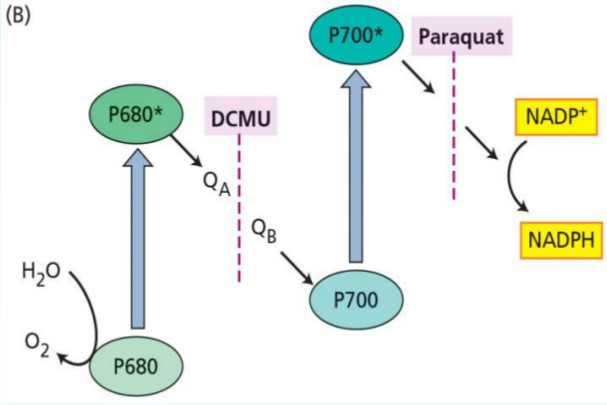
\includegraphics[scale=0.4]{immagini/erbicidi.jpg}
\caption{Siti di blocco della fotosintesi da parte di erbicidi}
\end{figure}

(3.12.14)

\chapter{Fase oscura fotosintesi}
L’organicazione della $CO_{2}$ avviene nello stroma del cloroplasto durante la fase oscura della fotosintesi.
Si completa la conversione energetica dell'energia luminosa e vengono sintetizzati scheletri carboniosi. I
carboidrati prodotti sono utilizzabili per i processi anabolici e catabolici delle piante.
Le reazioni di fissazione e riduzione della $CO_{2}$ richiedono ATP e NADPH, prodotti grazie alla luce.
Il processo metabolico universale per la fissazione e riduzione della $CO_{2}$ è il ciclo di Calvin, detto anche
ciclo C3 o PCRC (Photosynthetic Carbon Reduction Cycle).
\section{Ciclo di Calvin}
Il ciclo di Calvin riduce la $CO_{2}$ in carboidrati tramite il ciclo fotosintetico per la riduzione del carbonio. La $CO_{2}$ viene fissata mediante l'utilizzo di ATP e NADPH generati dalle reazioni alla luce. Il ciclo si articola in 3 fasi:
\begin{enumerate}
\item{Carbossilazione}
\item{Riduzione}
\item{Rigenerazione}
\end{enumerate}

\begin{figure}[H]
\centering
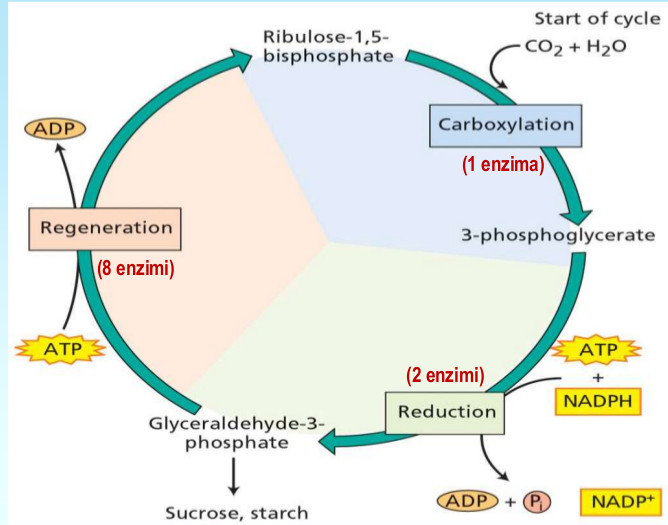
\includegraphics[scale=0.4]{immagini/calvin.jpg}
\caption{Le tre fasi del ciclo di Calvin}
\end{figure}
La $CO_{2}$ e l'acqua ottenuti dall'ambiente sono unite enzimaticamente a una molecola acettore a 5 atomi di C (\textbf{ribulosio 1,5-bisfosfato}) per generare due molecole di un intermedio a 3 atomi di C, il quale è ridotto in carboidrati utilizzando ATP e NADPH.
\subsection{Carbossilazione}
Tre molecole di $CO_{2}$ regiscono con tre molecole di ribulosio-1,5-bisfosfato per formare 6 molecole di \emph{3-fosfoglicerato}, grazie all'enzima RuBisCO (Ribulosio 1,5-Bisfosfato Carbossilasi-Ossigenasi). La rezione catalizzata dalla RuBisCO determina l’estrazione di un
protone dal ribulosio 1-5 bisfosfato promuovendo la formazione di un intermedio enediolato. Il successivo attacco
nucleofilo della $CO_{2}$ origina un intermedio $\beta$-cheto acido, che, reagendo con l’acqua, si idrolizza per dare due molecole
di acido 3-fosfoglicerico. RuBisCO è un enzima attivato dalla luce. 
\begin{figure}[H]
\centering
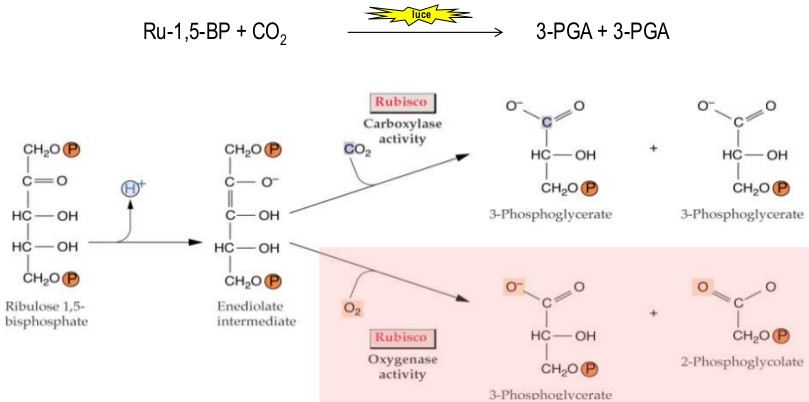
\includegraphics[scale=0.4]{immagini/carbossilazione.jpg}
\caption{Fase di carbossilazione}
\end{figure}
La formazione dei prodotti è favorita dalla grande carica negativa dell'energia libera associata alla carbossilazione del ribulosio e dall'affinità della RuBisCO per la $CO_{2}$, che assicura rapida carbossilazione alle concentrazioni basse.

\paragraph{RuBisCO}
Costituisce circa il 40\% delle proteine solubili della foglia. È la più abbondante proteina della biosfera
(107 t). La concentrazione di enzima attivo nella cellula è 4 mM (500 volte maggiore di quella della $CO_{2}$): in particolare, nel cloroplasto è 0.2 g/mL.
L’enzima è una grossa proteina con massa 560 kDa formata da 16 subunità:
\begin{itemize}
\item{8 pesanti (L = Large) (55 kDa ciascuna) codificate dal genoma cloroplastico}
\item{8 leggere (S = Small) (14 kDa ciascuna) codificate dal genoma nucleare, sintetizzate sui ribosomi
citoplasmatici, trasportate nel cloroplasto dove sono assemblate con le subunità pesanti}
\end{itemize}
Il sito catalitico si trova nelle subunità grandi: 1 sito per ciascuna.
L’enzima possiede due attività:
\begin{enumerate}
\item{Carbossilasica}
\item{Ossigenasica, come si vede nella figura sopra in rosa}
\end{enumerate}

L'alta affinità per la $CO_{2}$ e l'elevata concentrazione dell'enzima nel cloroplasto favoriscono la reazione di
carbossilazione anche a basse concentrazioni di $CO_{2}$ (nell'atmosfera la concentrazione di $CO_{2}$ è solo 360 ppm).
Le reazioni di carbossilazione e ossigenazione avvengono nello stesso sito catalitico dell'enzima: $CO_{2}$ e
$O_{2}$ sono substrati competitivi. 

Quale delle due reazioni prevale? Nelle normali condizioni atmosferiche (~ 21\% $O_{2}$, ~ 0,036\% $CO_{2}$) abbiamo un rapporto di \emph{3 carbossilazioni : 1 ossigenazione}; in atmosfera artificiale, fornendo uguali concentrazioni di $CO_{2}$ e $O_{2}$, il rapporto sale a \emph{80 carbossilazioni : 1 ossigenazione}.

Inoltre, la concentrazione di un qualsiasi gas disciolto in acqua è proporzionale alla sua pressione parziale
(Pgas) al di sopra della soluzione ed al suo coefficiente di assorbimento $\alpha$ (=volume di gas assorbito da
un volume di acqua alla pressione di 1 atmosfera e ad una determinata T). Siccome $\alpha$ è T dipendente,
diminuisce con l’aumentare di T. Sono riportati in tabella i valori delle concentrazioni di $CO_{2}$ e di $O_{2}$ a varie
temperature. Il rapporto [$CO_{2}$]/ [$O_{2}$] diminuisce con l’aumentare della T, pertanto viene favorita l'ossigenazione rispetto alla carbossilazione

\subsection{Riduzione}
Questa fase è costituita da 2 reazioni:
\begin{enumerate}
\item{Fosforilazione del 3-fosfoglicerato sul C carbossilico, con formazione di \textbf{1,3-bisfosfoglicerato}. La reazione è catalizzata dall'enzima \emph{3-fosfoglicerato chinasi} e spende ATP}
\item{Riduzione del 1,3-bisfosfoglicerato a \textbf{gliceraldeide-3-fosfato} con l'energia del NADPH, ad opera dell'enzima \emph{gliceraldeide-3-fosfato-deidrogenasi}\footnote{Simile a quello presente nella glicolisi, ma utilizza NADP invece che NAD}}
\end{enumerate}
\begin{figure}[H]
\centering
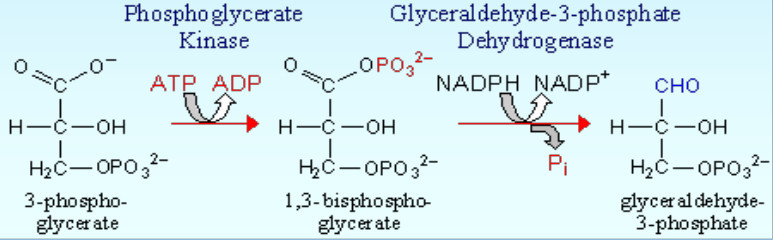
\includegraphics[scale=0.4]{immagini/riduzione.jpg}
\caption{Fase di riduzione}
\end{figure}

\subsection{Rigenerazione}
Affinchè gli intermedi del ciclo di Calvin non vengano esauriti, la fissazione della $CO_{2}$ ha bisogno che il suo accettore, il ribulosio-1,5-bisfosfato, venga costantemente rigenerato. Ciò avviene a partire da 5 delle 6 molecole\footnote{La sesta molecola rappresenta l'assimilazione netta delle 3 molecole di $CO_{2}$ e diventa disponibile per il metabolismo del C della pianta} di gliceraldeide-3-fosfato che si sono originate dalle due fasi precedenti:
\begin{figure}[H]
\centering
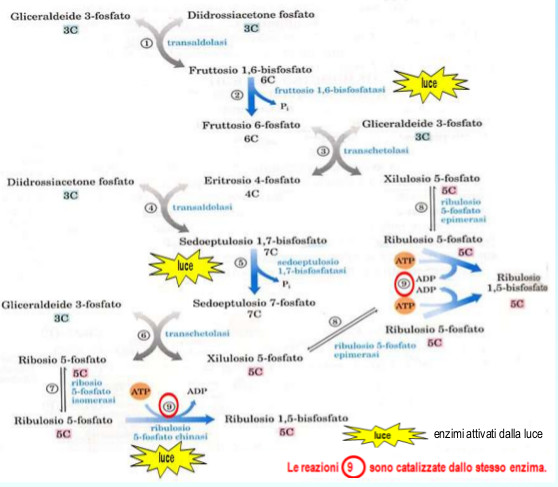
\includegraphics[scale=0.4]{immagini/rigenerazione.jpg}
\caption{Fase di rigenerazione}
\end{figure}

Nel dattaglio:
\begin{itemize}
\item{2 molecole di G3P sono convertite in \textbf{DHC-3P} (diidrossiacetone 3 fosfato) dalla \emph{trioso fosfato isomerasi}}
\item{1 molecola di DHC-3P va incontro a condensazione aldolica con la terza molecola di G3P, per formare \textbf{fruttosio-1,6-bisfosfato} grazie all'enzima \emph{aldolasi}}
\item{Il fruttosio-1,6-bisfosfato viene idrolizzato a \textbf{fruttosio-6-fosfato}}
\item{Il C-1 e il C-2 del F6P vengono trasferiti dall'enzima \emph{transchetolasi} sulla quarta molecola di $CO_{2}$, con formazione di \textbf{xilulosio-5-fosfato}. I rimanenti atomi di C formano \textbf{eritrosio-4-fosfato}}
\item{L'eritrosio-4-fosfato si combina con la restante molecola di DHC-3P a formare \textbf{sedoeptulosio-1,7-bisfosfato} grazie all'aldolasi}
\item{Il sedoeptulosio-1,7-bisfosfato viene idrolizzato da una \emph{fosfatasi} a formare \textbf{sedoeptulosio-7-fosfato}}
\item{Il sedoeptulosio-7-fosfato dona 2 C alla quinta molecola di G3P e produce un'altra molecola di \textbf{xilulosio-5-fosfato}}
\item{Le due molecole di xilulosio-5-P, grazie all'\emph{epimerasi}, sono convertite in due molecole di \textbf{ribulosio-5-P}}
\item{Il ribulosio-5-P, tramite la \emph{ribulosio-5-P chinasi}, viene convertito il \textbf{ribulosio-1,5-bisfosfato} utilizzando ATP}
\end{itemize}

\subsection{Stechiometria del ciclo di Calvin}
Quanto carbonio può essere esportato dal ciclo di Calvin e quanto ne deve essere utilizzato per
rigenerare l’accettore?

Su 6 molecole di G3P (18 C), soltanto 1 molecola (3 C) può essere esportata, mentre 5
molecole (15 C) sono riconvertite a Ru-1,5-BP.

Per sintetizzare un esoso, a livello energetico, sono necessarie 6 molecole di $CO_{2}$. Per ogni molecola di $CO_{2}$ servono 3 ATP e 2 NADPH: perciò, per ogni esoso servono 18 ATP e 12 NADPH. Ad esempio, per il \emph{saccarosio}, bisogna moltiplicare tutto per 2.

(10.12.2014)

\section{Regolazione del ciclo di Calvin}
Gli scheletri carboniosi devono essere sintetizzati quando sono presenti ATP e NADPH e $CO_{2}$. La percezione della luce da parte della cellula regola il ciclo di Calvin, il quale non funziona di notte perchè gli enzimi sono regolati dalla luce e perchè col buio gli stomi si chiudono. I meccanismi che regolano il ciclo sono 3:
\begin{enumerate}
\item{Regolazione in funzione della velocità alla quale il C è utilizzato per la sintesi dei carboidrati}
\item{Regolazione in funzione della luce attraverso alterazioni del pH dello stroma del cloroplasto, della concentrazione di Mg e dal sistema di tioredossine}
\item{Attivazione catalitica della RuBisCO}
\end{enumerate}

\subsection{Regolazione in funzione della velocità alla quale il C è utilizzato per la sintesi dei carboidrati}

Dipende dalla velocità con cui la pianta utilizza i prodotti finali. I trioso fosfati vengono usati per la sintesi di \emph{saccarosio}, che è solubile e mobile e permette il trasporto degli zuccheri nel circolo floematico (70 \%). Il 30 \% degli zuccheri prodotti viene utilizzato per la sintesi di \emph{amido}, che è insolubile e depositato nello stroma del cloroplasto in granuli, è osmoticamente inattivo ed è un'ottima forma di accumulo di zuccheri. Durante la notte l'amido viene mobilizzato per mantenere il metabolismo di base della cellula vegetale.

La produzione di amido è regolata da un meccanismo interno che dipende dall'attività di un traslocatore antiporto di triosi fosfati (fuori) e gruppi fosfato (dentro); questi ultimi rendono possibile  la sintesi di ATP necessaria a mantenere lo stato energetico della cellula per mantenere il ciclo di Calvin.
\begin{figure}[H]
\centering
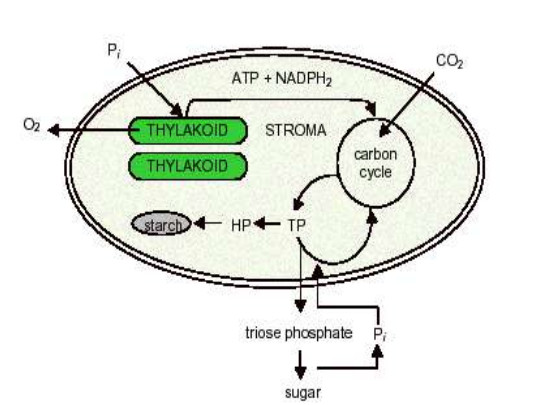
\includegraphics[scale=0.4]{immagini/reg.jpg}
\caption{Regolazione in funzione della velocità alla quale il C è utilizzato per sintesi di carboidrati}
\end{figure}

\emph{La velocità con la quale il C fuoriesce dal ciclo di Calvin è quindi controllata dalla velocità di sintesi dell’amido
nel cloroplasto e del saccarosio nel citosol.}

\subsection{Regolazione ad opera della luce}
Legato alla regolazione diretta da parte del pH dello stroma, della attivazione riduttiva di alcuni enzimi del ciclo di calvin e della disponibilità di ioni Mg nello stroma (servono per enzimi che catalizzano le fasi reversibili del ciclo, come la fruttosio 1,6-bisfosfatasi, la ribulosio fosfatasi e la sedoeptulosio 1,7-bisfosfatasi, che sono attivati direttamente dalla luce).

Lo stroma si alcalinizza e il lume del cloroplasto si acidifica. Gli enzimi, inattivi al buio, divengono attivi conseguentemente alla traslocazione di protoni legata alla catena di trasferimento elettronico (in particolare al plastochinone), sia conseguentemente all'aumento di ioni Mg nello stroma per controbilanciare la perdita di cariche + al momento della loro traslocazione nel lume.
\begin{figure}[H]
\centering
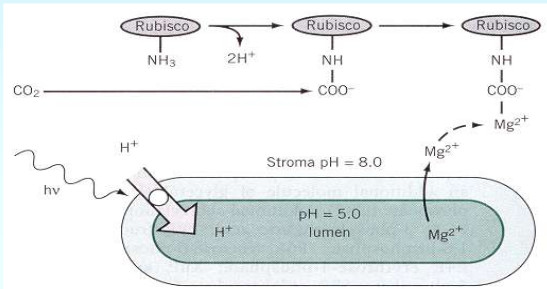
\includegraphics[scale=0.4]{immagini/reg1.jpg}
\caption{Regolazione in funzione della luce}
\end{figure}
La concentrazione di Mg nello stroma aumenta
da 1-3 mM a 3-6 mM. Inoltre l’immissione di protoni nel lume determina l’alcalinizzazione (pH 8) dello
stroma.
Anche la presenza di ATP e NADPH attivano questi enzimi.

La \emph{RuBisCO} è a sua volta regolata da questi fattori: necessita di pH intorno ad 8.

\paragraph{Regolazione da parte della luce mediante ferridossina-tioredossina}
Le tioredossine sono proteine che, alla luce, vengono ridotte dalla ferridossina. La ferridossina ridotta agisce indirettamente riducendo queste tioredossine per ridurre gli enzimi, riducendo i ponti disolfuro e quindi liberando residui di Cys. Le tioredossine poi riducono gli enzimi target del ciclo di Calvin.
\begin{figure}[H]
\centering
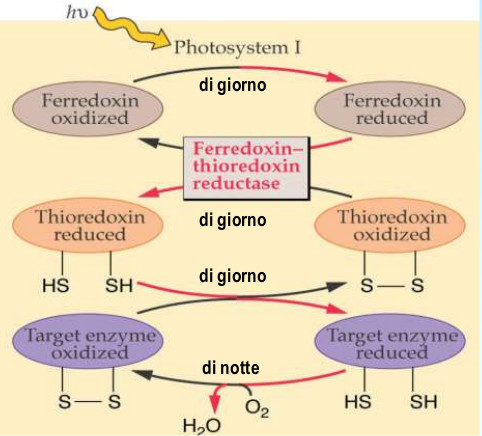
\includegraphics[scale=0.4]{immagini/reg2.jpg}
\caption{Regolazione in funzione della luce mediante ferridossina e tioredossina}
\end{figure}
\subsection{Regolazione per attivazione catalitica della RuBisCO}

Per la sua attività è necessario che l'enzima sia \emph{carbammilato}. L'enzima è inattivato al buio dalla presenza del substrato (ribulosio 1,5-bisfosfato) e da un analogo dell'intermedio della reazione, il \emph{carbossiarabinitolo 1-P}, che è un inibitore. Essi si legano al sito attivo dell'enzima, inattivandolo. 
\begin{figure}[H]
\centering
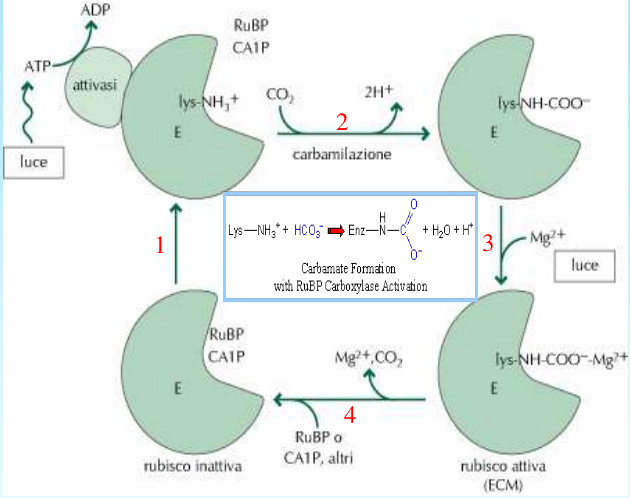
\includegraphics[scale=0.4]{immagini/reg4.jpg}
\caption{Regolazione per attivazione catalitica della RuBisCO}
\end{figure}
Durante il giorno, l'inibitore viene rimosso da una fosfatasi, che lo defosforila e ne disattiva l'azione di inibitore. La \emph{RuBisCO attivasi} durante il giorno utilizza l'ATP prodotto dalla fase luminosa della fotosintesi per legarsi alla RuBisCO, generando una modificazione conformazionale tale per cui un residuo di Lys nel sito attivo della RuBisCO può legare una molecola di $CO_{2}$, che funziona da attivatore allosterico: si forma il derivato carbammilato che può legare Mg.

Durante la notte, mancando ATP, la RuBisCO attivasi non si lega e RuBisCO è inattiva.

\section{Fotorespirazione}
Detto anche \emph{ciclo C2}, porta all'ossidazione fotosintetica del carbonio.
È un processo metabolico respirativo che le piante con ciclo C3 attuano alla luce, e continuano per un breve periodo anche al buio, per eliminare l'ossigeno in eccesso.

Le alte pressioni di ossigeno atmosferico provocano uno stop della fotosintesi, al fine di prevenire la formazione di radicali liberi, dannosissimi alle cellule; via via che queste pressioni diminuiscono, in favore della pressione cellulare di anidride carbonica, il processo fotosintetico aumenta la sua attività.

Consumo di ossigeno ed evoluzione di $CO_{2}$ stimolati dalla luce: essi sono in competizione perchè entrambi substrati della RuBisCO\footnote{La RuBisCO è infatti capace di catalizzare sia la carbossilazione che l'ossidazione del ribulosio-1,5-bisfosfato}. Il consumo di ossigeno è più evidente ad alte temperature, poichè l'ossigeno è più solubile in acqua ad alte temperature rispetto alla $CO_{2}$. $CO_{2}$ ed $O_{2}$ sono substrati \emph{competitivi}.

Due atomi di C saranno impiegati per la produzione di Ser e di \textbf{2-fosfoglicolato}, che si forma nel cloroplasto a seguito dell'ossigenazione del ribulosio-1,5-bisfosfato. Questo viene idrolizzato a \textbf{glicolato}e infine convertito nel perossisoma in \emph{glicina} ad opera della catalasi.

La glicina va nel mitocondrio e viene carbossilata a Ser, che a sua volta torna nel perossisoma, viene convertita a \emph{idrossipiruvato} per messo di una transamminazione. L'idrossipiruvato viene a sua volta trasformato in  \emph{glicerato} tramite una reduttasi NADH-dipendente e che va nel cloroplasto, dove viene fosforilato a \emph{3-fosfoglicerato} e rientra nel ciclo di Calvin.
\begin{figure}[H]
\centering
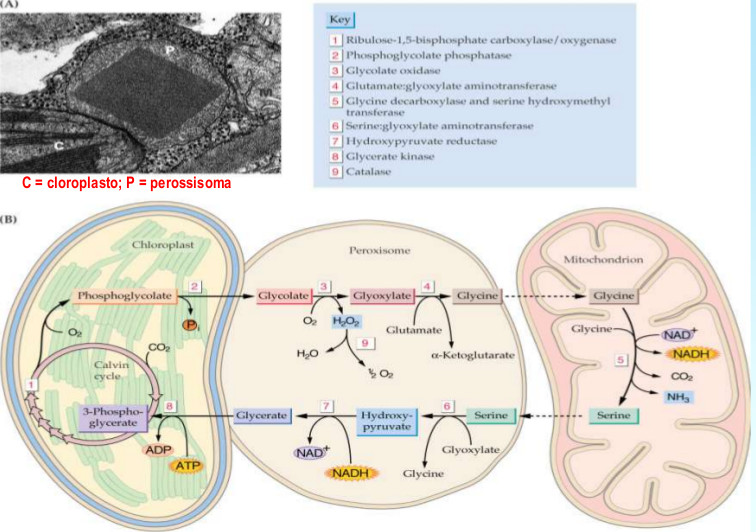
\includegraphics[scale=0.4]{immagini/c2.jpg}
\caption{Fotorespirazione o ciclo C2}
\end{figure}
Il ciclo fosforespiratorio dipende dal ciclo di Calvin: quello di Calvin utilizza e rigenera autonomamente il ribulosio 1,5 bisfosfato e la $CO_{2}$; quello fosforespiratorio impiega ossigeno con la reazione della RuBisCO ed è un parassita del ciclo di Calvin per il 2-fosfoglicolato. Esso entra nel ciclo fotorespiratorio, viene rilasciata $CO_{2}$, che comunque viene compensata attraverso il ciclo C2. In realtà una sola molecola di C viene recuperata perchè durante la respirazione viene persa un'altra $CO_{2}$. 

Il ciclo C2 è attivo soltanto alla luce
perché, richiedendo energia, dipende
dal trasporto fotosintetico degli e- per:
\begin{itemize}
\item{ATP: per convertire glicerato a 3-P-
glicerato (reazione 3.10 nel cloroplasto)}
\item{ATP e $Fd_{red}$: per riassimilare lo $NH_{4}^{+}$
prodotto nel mitocondrio }
\end{itemize}

\subsection{Gli organuli}
Cloroplasto, perossisoma e mitocondiro. Nel mesofillo fogliare essi sono in prossimità l'uno rispetto all'altro. I metaboliti vanno dal cloroplasto al perossisoma al mitocondrio, nel quale vengono modificati e tornano al cloroplasto.

Dal 2-fosfoglicolato, prodotto grazie alla RuBisCO, si produce glicolato che nel perossisoma viene ossidato al glicossilato e poi a glicina, che va nel mitocondrio e viene trasformata in serina (perdita di $CO_{2}$). La serina percorre la strada inversa.

La fosforespirazione non è un ciclo autonomo, è associato al ciclo di Calvin, nel quale c'è guadagno netto di carbonio. Nel ciclo C2 (fosforespiratorio) c'è invece una perdita di carbonio.
\\
Così come il Ciclo di Calvin, anche il ciclo C2 dipende dalla luce, poichè l'attività della RuBisCO ne dipende: essa si attiva quando c'è Mg e ATP, necessario alla funzione della RuBisCO attivasi, che rende la RuBisCO asuscettibile all'attacco della $CO_{2}$. Questa energia è prodotta durante la fase luminosa della fotosintesi.

Si ha produzione di uno ione ammonio che viene, nel cloroplasto, incorporato nel ciclo GS-GoGat per la sintesi di Glu e Gln. 
L'ultimo passaggio del ciclo C2 è la fosforilazione del glicerato a formare 3-fosfoglicerato: serve ATP, così come serve per la sintesi di Gln da Glu.

\subsection{Fase 1}
Dal cloroplasto al perossisoma al mitocondrio.

La prima reazione porta alla sintesi di 2-fosfoglicolato, il quale ha 2 C e non può entrare nel ciclo di Calvin: viene quindi defosforilato con produzione di \emph{glicolato}. Considerando che l'involucro del cloroplasto non è permeabile alla maggior parte dei composti di questo ciclo, sebbene lo sia abbastanza a molecole neutre anche piuttosto grandi, esistono dei traslocatori specifici: uno scambia in maniera stechiometrica 1:1 il glicolato (verso il perossisoma) e il glicerato (dal perossisoma al cloroplasto, sarà fosforilato dopo). 

2 molecole di glicolato vengono modificate nel \emph{perossisoma}: la glicolato ossidasi le converte in \emph{gliossilato}. Intervengono due molecole di  $O_{2}$ e si forma $H_{2}O_{2}$, tossica, che viene scissa dalla catalasi in una molecola di $O_{2}$ e 2 molecole di acqua. Questo ossigeno è una delle 3 molecole di ossigeno che entrano nel ciclo C2: è una delle due che vengono usate per ossidazione del glicolato.

2 molecole di glicossilato vengono convertite in 2 molecole di \emph{glicina} per trasnaminazione del Glu, si forma 2-ossoglutarato che servirà o nel cloroplasto per il ciclo GS-GOGAT o nelle transaminazioni nel perossisoma.

Gly viene traslocata nel mitocondrio: 2 molecole di glicina vengono convertite in una molecola di Ser con rilascio di 1 $CO_{2}$, grazie agli enzimi \emph{glicina decarbossilasi} e \emph{serina idrossimetil transferasi}.
La prima molecola di Gly viene scissa in $CO_{2}$, $NH_{3}$, NADH (perchè l'enzima usa NAD) e un gruppo metilenico, che si forma per azione dell'enzima \emph{metilene folato}. Questo composto traferisce un C grazie alla serina-idrossimetil transferasi \lfreccia otteniamo THF (tetraidrofolato) e Ser.  

L'ammonio verrà eliminato dalla cellula trasferendolo al cloroplasto, dove verrà impiegato nella sintesi di aa tramite il ciclo GS-GOGAT.

\subsection{Fase 2}
Dal mitocondrio al perossisoma al cloroplasto.

La serina viene, nel persossisoma, deaminata a \emph{idrossipiruvato}, che viene poi ridotto a glicerato grazie all'enzima \emph{idrossipiruvato riduttasi}, con consumo di NADH.
 Il glicerato va nel cloroplasto e viene fosforilato ad opera della glicerato chinasi a \emph{3-fosfoglicerato}, che può entrare nel ciclo di Calvin. L'ammonio viene incorporato sul Glu a formare Gln, e poi per aminotransferasi va a formare 2 Glu.
 
La stechiometria del ciclo C2 è molto complessa. Tuttavia il costo energetico del ciclo C2
viene valutato pari a 2 ATP e 2 $Fd_{red}$ (o 1 NADPH).
Considerando il costo energetico per fissare e ridurre la $CO_{2}$ liberata e la rigenerazione del
Ribulosio 1,5 BP dal 3-PGA, si arriva a circa\textbf{5 ATP} e \textbf{3 NADPH}. 
 
\paragraph{Traslocatore malato-2-ossoglutarato}
Traslocatore di potere riducente. Il malato viene ridotto nel cloroplasto utilizzando NADPH e poi traslocato all'esterno, ossidato con produzione di\todo{Che roba è??????????}

 
\subsection{Funzioni fotorespirazione} 
\begin{enumerate}
\item{Recupero del C che verrebbe perso dall'ossigenazione del ribulosio-5-fosfato da parte della RuBisCO. Il 75\% viene recuperato nel fosfoglicerato, il restante è perso nella $CO_{2}$}

\item{Diminuisce l'efficienza fotosintetica della fissazione di C:se l'efficienza fotosintesica è intorno al 90 \%, conseguentemente alla fotorespirazione può scendere fino al 50 \% a seconda delle condizioni ambientali (alta T, bassa idratazione)}

\item{La fotorespirazione è comunque un processo necessario alle piante. Mutanti di Arabidopsis incapaci di fotorespirare, non sopravvivono alle condizioni atmosferiche attuali (aerobiche). Questi mutanti vengono riconosciuti una volta che le piante si trovano in condizioni di ambienti atmosferici normali, con basse concentraziondi di  $CO_{2}$ rispetto a ossigeno\footnote{Non si sa perchè la fotorespirazione sia un processo necessario: si suppone che ci siano effetti collaterali come recupero di C, alto impiego di ammonio e che funzioni per attenuare gli eccessi di potere riducente}}
\item{In condizioni di alti livelli di irradianza e ridotti scambi gassosi, si ha un rallentamento del ciclo di Calvin e il NADPH si accumula. La $CO_{2}$ diventa limitante. La fotorespirazione potrebbe utilizzare questo NAPDH (cosa che accade) e sbloccare la fase luminosa della fotosintesi}
\end{enumerate} 

\paragraph{Quanto C assimilato viene liberato come $CO_{2}$ a seguito della rezione di ossigenazione della RuBisCO?}
Dipende dalle velocità di carbossilazione ed ossigenazione: sono regolate dai livelli di concentrazione dei due gas $CO_{2}$ e ossigeno. 

Le due concentrazioni sono diverse nell'atmosfera e nell'acqua:
\begin{itemize}
\item{Nell'atmosfera la $CO_{2}$ è 600 volte meno concentrata dell'ossigeno \lfreccia favorita l'ossidazione} \item{Nell'acqua la concentrazione di $CO_{2}$ è molto più bassa rispetto all'atmosfera e solo 25 volte inferiore rispetto all'ossigeno: il rapporto [$CO_{2}$]/[$O_{2}$] è più alto rispetto all'aria \lfreccia favorita la carbossilazione}
\end{itemize}

La concentrazione dei gas dipende dalla \emph{temperatura}: all'aumentare di T, la RuBisCO ha un'affinità maggiore per $O_{2}$ \lfreccia favorita l'ossidazione.

\paragraph{}
Tutte le piante effettuano C3, poche C4 e CAM. Queste ultime sono adattate ad ambienti caldi ed aridi: le piante sono costrette a tenere chiusi gli stomi durante il giorno, quando la traspirazione è massima. Esse effettuano due tipi di carbossilazione: la prima  avviene in condizioni di $CO_{2}$ limitante e non è operata dalla RuBisCO. Queste piante evitano di fatto la fotorespirazione.

\section{Destino degli zuccheri prodotti dal ciclo di Calvin}

Il saccarosio viene prodotto principalmente a seguito dell'organicazione del carbonio: alcuni esosi fosfati vengono impiegati nella sintesi di \emph{amido}.
La maggior parte degli zuccheri prodotti nelle foglie immature vengono impiegati localmente: poco saccarosio verrà esportato o usato per produrre amido.

Le foglie mature invece contribuiscono alla composizione della linfa floematica esportando il saccarosio, il quale è esportato alle varie parti della pianta secondo il meccanismo \emph{sorgente-pozzo}: gli organi pozzo non sono fotosinteticamente attivi o sono le radici che hanno bisogno di energie e richiamano saccarosio dalle sorgenti (foglie mature). Nei tessuti pozzo il saccarosio verrà usato sia per energia che per zucchero di riseva che per la crescita.

Durante la notte, l'amido transitorio viene scisso nei componenti: fruttosio e glucosio, vengono esportati nel citoplasma (esosi fosfati).

Perchè si usa il \emph{saccarosio} come zucchero di trasporto? È un disaccaride molto solubile in acqua, elettroneutro e gli organi sono in grado di metabolizzarlo ed impiegarlo nelle reazioni metaboliche che necessitano di glucosio e fruttosio.

La molecola si trova nel floema, e sarà utilizzato solo dove c'è il sistema enzimatico in grado di scinderlo. Decidere come e quando sintetizzare saccarosio e/o amido è un problema: la sintesi di amido e quella di saccarosio sono regolate dai livelli di Pi presenti nel citosol\footnote{l'amido viene sintetizzato nello stroma del cloroplasto, mentre la sintesi del saccarosio avviene nel citosol.}.

La concetrazione di Pi agisce sul \emph{traslocatore dei fosfati}, che si trova all'interno del cloroplasto e scambia i triosi fosfati con Pi. Importa Pi dal citosol ed esporta triosi fosfati. Se nel citosol la concetrazione di Pi è alta, i triosi fosfati sono esportati dal cloroplasto al citosol ed impiegati per la sintesi di saccarosio. Se invece è bassa, i triosi fosfati vengono trattenuti nel cloroplasto dove sono utilizzati per la sintesi di amido.

Questo traslocatore è molto abbondante nell'involucro interno del cloroplasto (15\% delle proteine). 6 eliche transmembrana, di cui la quinta prensenta Arg e Lys che sembrano essere coinvolte nel legame dei substrati. Il traslocatore ha affinità anche per altri substrati, però le Km sono più alte di quelle per i triosi fosfati.Esso media la distribuzione dei Pi ai due lati della membrana, determinando la sintesi di saccarosio o di amido.

Nel cloroplasto ci sono vari traslocatori:
\begin{itemize}
\item{Traslocatore dei triosi fosfati : scambia fosfato inorganico del citosol con triosi fosfati dello stroma}
\item{Traslocatore acidi bicarbossilici : scambia acidi bicarbossilici (malato, succinato, ecc.) tra il
cloroplasto e il citosol; ruolo nel trasferimento indiretto di equivalenti riducenti}
\item{Traslocatore ATP/ADP : scambia ATP/ADP tra citoplasma e citosol; ruolo nel fornire ATP al
cloroplasto in fase di inattività fotosintetica (notte)}
\item{Traslocatore glicolato/glicerato : scambia i due metaboliti della fotorespirazione}
\end{itemize}
\paragraph{Saccarosio}
Glucosio + fruttosio \lfreccia saccarosio (reazione reversibile)
\begin{figure}[H]
\centering
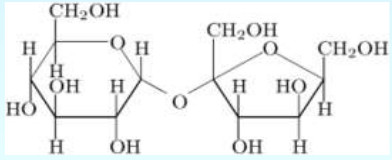
\includegraphics[scale=0.4]{immagini/saccarosio.jpg}
\caption{Struttura del saccarosio}
\end{figure}

\subsection{Sintesi di saccarosio}

La sua sintesi a partire dai \emph{triosi fosfati} vede la formazione di fruttosio 1,6 bisfosfato, la sua defosforilazione a 2 molecole di fruttosio 6-P, che seguono due vie diverse: uno viene usato dalla saccarosio fosfato sintasi per formare saccarosio e uno viene convertito in glucosio 6-P, poi glucosio 1-P e poi a UDP-glucosio, la forma attiva del glucosio per la sintesi del saccarosio.

(18.02.2015)
\begin{figure}[H]
\centering
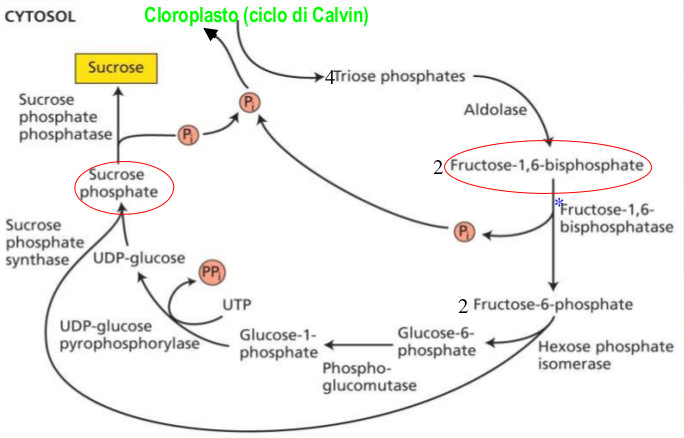
\includegraphics[scale=0.4]{immagini/saccarosio1.jpg}
\caption{Sintesi del saccarosio}
\end{figure}

La sintesi del saccarosio avviene nel \emph{citoplasma}: i triosi fosfati prodotti alla fine del ciclo di calvin dovranno essere trasportati nel citoplasma dal cloroplasto; ciò avviene scambiandoli con il Pi. Questo dipende dall'attività del fruttosio-1,6-bisfosfato, intermedio della sintesi del saccarosio e della glicolisi.

Il \textbf{fruttosio 1,6-bisfosfato} inibisce la sintesi, tramite la fruttosio 1,6 bisfosfatasi, e attiva la fosfofruttochinasi: inibisce quindi la sintesi del saccarosio e si forma il \textbf{fruttosio-6-fosfato}.

La fruttosio 6-fosfato chinasi converte il fruttosio 6-P in \textbf{fruttosio 2,6 bisfosfato}: esso è un regolatore della sintesi di saccarosio, in quanto inibisce la fruttosio 1,6 bisfosfatasi, attiva la fosfofruttochinaso ed è convertito dalla fruttosio 2,6 bisfosfatasi in fruttosio 6-P.

La chinasi è attivata da alte [Pi] ed
inibita da alte [triosiP], mentre la fosfatasi è attivata da alte [triosiP] ed inibita da da alte [Pi].

Nel momento in cui la sintesi di saccarosio rallenta perchè rallenta la necessità della pianta di impiegare questo composto, si riduce il pool di fosfato inorganico nel citosol \lfreccia riduzione traslocazione dei triosi fosfato dai cloroplasti al citosol \lfreccia ristagno triosi fosfati.

\paragraph{Amido}
L'amido nei granuli costituisce una forma semi-cristallina \lfreccia rifrangenza. L'aspetto cristallino del granulo dipende dalle modalità in cui è sintetizzato e da come l'amilosio e l'amilopectina vengono distribuiti al suo interno.

Una delle caratteristiche dell'\emph{amilosio} è che il polimero ha una struttura D ad elica: la dimensione dell'elica favorisce il legame con lo iodio, che determina il viraggio della colorazione a rosso-viola.

L'\emph{amilopectina} è ramificata: le catene laterali sono unite alla principale mediante legami $\alpha$ 1\freccia6. Il grado di polimerizzazione è più variabile: catene molto più lunghe rispetto all'amilosio.

L'amilosio è in genere meno rappresentato dell'amilopectina.

\subsection{Sintesi di amido}

I triosi fosfati sintetizzati sono prima indirizzati alla sintesi di saccarosio. Al momento in cui la necessità di saccarosio da parte dei tessuti periferici si riduce, si ha il rallentamento della sintesi e l'accumulo di triosi fosfato all'interno del cloroplasto e la sintesi di amido (durante il giorno!).

L'amido è una riserva prolungata nel tempo. Di notte viene degradato per soddisfare le richieste dei metaboliti per la respirazione.

 
 (23.02.2015)
 
 \chapter{Fotoinibizione}
 Un processo che avviene quando la pianta vive in condizione di prolungata ed elevata irradianza (la luce è eccessiva per le capacità fotosintetiche della pianta). Essa va incontro ad eventi più o meno dannosi.
 
 La fotoinibizione comporta uno \emph{stallo} del sistema di trasporto elettronico della fase luminosa della fotosintesi. 
 
 La fotossidazione è a carico delle molecole di clorofilla che, ricevendo troppa energia, non riescono ad eliminarla \lfreccia molecole eccitate in tripletto \lfreccia ossidazione dei pigmenti \lfreccia perdita di pigmentazione della foglia.
 
Le piante devono essere in grado di minimizzare l'assorbimento di luce per evitare questi fenomeni.
Nel caso di fotoinibizione i fotosistemi sono incapaci di trasferire energia della radiazione luminosa ai trasportatori elettronici associati alla membrana tilacoidale. Ciò si verifica quando la fase luminosa procede troppo velocemente rispetto alla fase oscura.

Se il ciclo di Calvin va lento, non vengono impiegati NADPH ed ATP prodotti a livello del fotosistema 1: non utilizzarli significa che non vengono rigenerate le molecole che sono gli accettori finali, ovvero NADP+ e ADP (per la sintesi di ATP) \lfreccia \emph{stallo della catena di trasporto}. Ciò si verifica con elevati livelli di irradianza per periodi prolungati, oppure quando non c'è $CO_{2}$ per l'organicazione del carbonio, ad esempio in condizioni di stress idrico.

Quando c'è molto fotosistema 2 rispetto all'1, avendo un complesso antenna più grande esso capta più luce, e quindi la fotoinibizione è più probabile.

Quando il ciclo di Calvin rallenta, il NADPH non viene ossidato e viene a mancare l'accettore finale (NADP+), così come l'ADP: se non viene sintetizzato ATP, si dissipa anche il trasporto elettronico attraverso la membrana. Si ha un \emph{blocco della catena respiratoria a livello del fotosistema 2}.

Se non c'è NADP+, si usa l'ossigeno: si produce il radicale superossido\footnote{la ferridossina riduce l'ossigeno con produzione del radicale superossido} che deve essere ridotto, perchè tossico. Esso entra nella \emph{via Asada-Halliwell}: viene convertito in perossido di idrogeno, che viene ulteriormente ridotto ad acqua, con formazione di composti che permetteranno il passaggio di elettroni dal perossido di idrogeno ad \emph{ascorbato}; l'ascorbato viene trasformato, grazie al glutatione ridotto, che diventa glutatione ossidato, e poi ridotto dalla ascorbato perossidasi. Questa reazione sortisce due effetti importanti che favoriscono lo sblocco della fotoinibizione.

La componente maggiormente coinvolta è il fotosistema 2, il quale può subire danni più o meno gravi a seconda del tempo di esposizione alla luce. Il danno può essere reversibile (fotoinibizione dinamica) o irreversibile (fotoinibizione cronica).

\section{Fotoinibizione dinamica}
Si osservano modifiche del fotosistema a livello dell'interazione del complesso antenna e PQH2. I due sono associati con interazioni di tipo elettrostatico, che vengono perturbate in uno dei meccanismi che servono a riparare la fotoinibizione: il PQH2 si accumula nello stroma, attivando una chinasi associata alla membrana tilacoidale che fosforila il LHC II. Questa fosforilazione perturba le interazioni e \emph{l'antenna si dissocia}, andandosi a legare al fotosistema 1. A questo punto il fotosistema 1 ha una bella antenna che gli permette di dissipare l'energia accumulata nel plastoidrochinone (PQH2) grazie al trasporto ciclico dell'elettrone, che utilizza come accettore di elettroni non più il NADP+ ma il \emph{plastochinone}.

Se i livelli di irradianza si abbassano, il plastochinone si scarica, riprende la propria forma chinonica: si ha un'attivazione di una fosforilasi presente nella membrana tilacoidale, che defosforila il complesso antenna, il quale si stacca e torna nel fotosistema 2.

Oppure si osservano modifiche nella struttura 3D del fotosistema 2 a livello del \emph{core complex}: alla fine non si ha la produzione dei grandi livelli di plastochinone dell'esempio precedente. Si modificano i siti di legame della proteine D1, e quindi un rallentamento del passaggio di elettroni dal plastochinone A al B.

\section{Fotoinibizione cronica}
La proteina D1 subisce un danno, riconosciuto da enzimi proteolitici, che la degradano \lfreccia fine dell'attività del fotosistema danneggiato. Esiste però un sistema continuo di sintesi proteica che ripristina la proteina D1. Il recupero della funzionalità dipende dall'entità del tasso di sintesi rispetto a quello di degradazione.

La chaperonina HSP70B protegge la proteina D1 dalla degradazione: una volta riconosciuta l'alterazione, lega D1 ed impedisce l'accesso agli enzimi proteolitici. Quando i livelli di irradianza diminuiscono, HSP70B si stacca.

HSP70B può anche legarsi al PSII stabilizzandolo, in modo da coordinare la degradazione di D1 danneggiata con sintesi di nuova D1.

Oppure, con bassi livelli di HSP70B, non si blocca la degradazione di D1: tutti i componenti di PSII si destabillizzano e tutti i componenti si disgregano.

\subsection{Altri meccanismi protettivi}
 
Ci son dei \emph{pigmenti}, come i carotenoidi, che spengono l'eccitazione sia delle clorofille (sia il tripletto che il singoletto di ossigeno) disperdendo l'energia in eccesso sotto forma di calore.

Un altro meccanismo è legato alle \emph{Xantofille}, che danno luogo al Ciclo delle Xantofille che può portare a dissipazione di energia eccessiva sotto forma di calore. A basse intensità è presente la violaxantina,  ad alte la zeaxantina. Non è chiaro come venga disperso il calore: c'è però interconversione tra i tre pigmenti. La zoaxantina è la più efficace nella dispersione di energia.

A mezzogiorno (alta irradianza) si ha riduzione dei livelli di violaxantina a favore della altre due xantofille.

Alte Xantofille sono coinvolte in questo processo, in particolare \emph{Luteina} e \emph{Neoxantina}.

Quello che sembra essere fondamentale nel processo di dissipazione è una \emph{modifica conformazionale di molecole di pigmento che si avvicinano alla clorofilla e la rendono in grado di accettare elettroni}, mediate da cambiamenti di pH a livello dello stroma.

\chapter{Fotosintesi CAM e C4}
Sono piante che hanno un metabolismo alternativo.
\section{C4}
Dette C4 perchè il primo prodotto stabile della fotosintesi è un composto a 4 atomi di C. Sono piante C4 \emph{Zea Mays}, detta volgarmente granoturco, e \emph{Saccharum officinarum}, detta volgarmente canna da zucchero.

Le foglie C3 e le foglie C4 differiscono:
\begin{figure}[H]
\centering
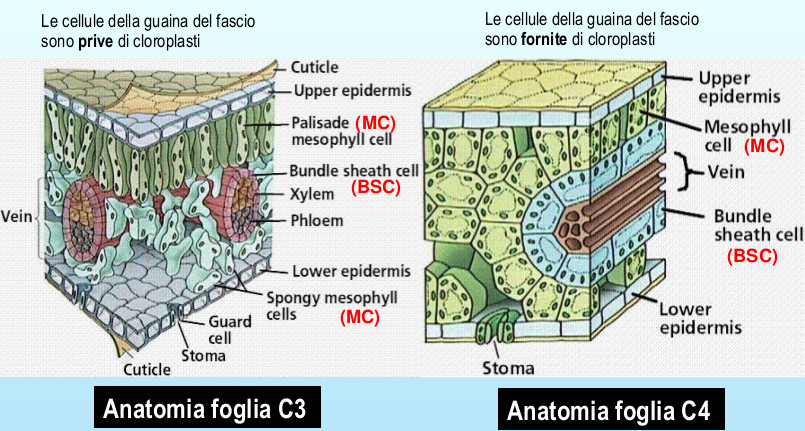
\includegraphics[scale=.4]{immagini/C4.jpg}
\caption{Confronto tra foglia C3 e foglia C4}
\end{figure} 
In una sezione trasversale della
foglia, le cellule intorno al fascio vascolare
formano una corona e sono chiaramente
diverse dalle cellule del mesofillo. I
cloroplasti delle cellule della guaina del
fascio sono significativamente più grandi di
quelli delle cellule del mesofillo.

Nelle cellule del mesofillo assistiamo alla carbossilazione per fosfoenolpiruvato, ad opera della \emph{PEP carbossilasi} e grazie alla $CO_{2}$ atmosferica. Si forma un composto a 4 atomi di C, che attraverso i plasmodesmi passa nelle cellule della guaina del fascio: qui viene decarbossilato ad opera dell'\emph{enzima decarbossilante}. La $CO_{2}$ entra nel ciclo di Calvin, mentre il composto a 3 C torna nelle cellule del mesofillo, dove viene riconvertito in fosfoenolpiruvato ad opera della \emph{piruvato fosfato dichinasi}.

Le cellule della guaina del fascio sono impermeabili ai gas, quindi non assorbono la $CO_{2}$ atmosferica, né assorbono l'ossigeno.
\subsection{Enzima decarbossilante}
Ci sono 3 tipi di enzima decarbossilante, che differiscono per la localizzazione della decarbossilazione, e che individuano 3 sottotipi di specie C4:
\begin{enumerate}
\item{  Enzima malico-NADP : nel  cloroplasto}
\item{Enzima malico NAD : nel mitocondrio}
\item{PEP-carbossichinasi : nel citosol}
\end{enumerate}
\begin{figure}[H]
\centering
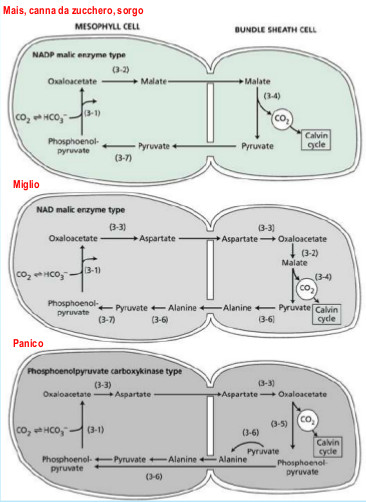
\includegraphics[scale=.4]{immagini/metabolismo.jpg}
\caption{I tre tipi di metabolismo C4}
\end{figure} 

\subsection{Enzima malico NADP} 
La carbossilazione del fosfoenolpiruvato (PEP) porta alla formazione dell'ossalacetato OAA, che viene convertito in malato grazie alla \emph{malato deidrogenasi} (riduzione di 1 NADP+ a NADPH) ed esportato alle cellule della guaina del fascio. La carbossilazione avviene nel cloroplasto ad opera dell'enzima malico, che utilizza una molecola di NADP+: la $CO_{2}$ va nel ciclo di Calvin e si forma \emph{piruvato}. Il piruvato viene trasportato nelle cellule del mesofillo e convertito in PEP, con spesa di 1 ATP.

\begin{figure}[H]
\centering
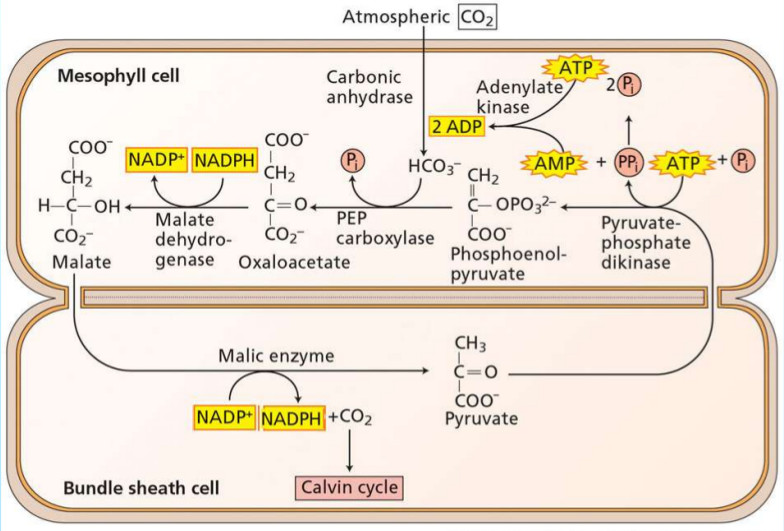
\includegraphics[scale=.3]{immagini/malico.jpg}
\caption{Metabolismo da enzima malico NADP}
\end{figure} 
Nelle specie a enzima NADP-malico, le cellule del fascio hanno generalmente cloroplasti agranali.

La PEP-carbossilasi è localizzata nel citosol delle cellule del mesofillo ed è attivata dalla luce. Ha come
substrati il PEP e lo HCO3-. L’alta affinità dell’enzima per lo HCO3- gli permette di catalizzare la
carbossilazione ad una bassa pressione parziale ($C_{i}$ = 10 Pa) di $CO_{2}$, che è meno della metà di quella
presente nel mesofillo di piante C3.

(2-03-2015)

La PEP carbossilasi lega il gruppo CO al PEP, con formazione di OAA, il quale viene trasferito sotto forma di malato alle cellule della guaina del fascio.
Il malato lì è poco concentrato rispetto alle cellule del mesofillo.  Il gradiente di malato si forma a causa della alta attività della \emph{malato deidrogenasi} nel mesofillo; nelle cellule della guaina del fascio l'enzima malico converte rapidamente il malato in piruvato. L'enzima malico usa NADP+: si producono $CO_{2}$ e NADPH. La $CO_{2}$ è estremamente concentrata nelle cellule della guaina del fascio e viene usata dalla RuBisCO per far partire il ciclo di Calvin. Questa elevata concentrazione
di $CO_{2}$ fa si che RuBisCO funzioni essenzialmente da \emph{carbossilasi} e che la \emph{fotorespirazione
sia praticamente annullata}.

Il piruvato va nel mesofillo, dove è subastrato della piruvato disfosfato chinasi, che forsforila il piruvato: si forma fosfoenolpiruvato, PPi ed AMP (perchè utilizza ATP). L'AMP viene usata dall'adenilato chinasi per sintetizzare due molecole di ADP, utilizzando ATP.
 
 \paragraph{Riassumendo}
Tutta l'attività metabolica serve per \emph{concentrare la $CO_{2}$ nei pressi della RuBisCO, per favorirne solo l'attività carbossilasica nelle cellule della guaina del fascio}.  L'assimilazione di $CO_{2}$ nelle piante C4 è alta anche a basse pressioni parziali, quindi è più efficiente. L'aumento della pressione parziale della $CO_{2}$ consente alla RuBisCO di avere solo attività carbossilasica.

Le cellule della guaina del fascio non rappresentano un sistema di reazioni alla luce completo rispetto alle cellule del mesofillo.

Il malato, per gradiente di concentrazione, diffonde nelle cell della guaina del fascio, dove viene decarbossilato \lfreccia qui la concentrazione di $CO_{2}$ aumenta \lfreccia si considera un \emph{pompaggio attivo} del gas.

\paragraph{Da dove viene in NADPH?}
Per ridurre la $CO_{2}$ nel ciclo di Calvin nelle cellule della guaina del fascio serve NADPH: infatti dalla decarbossilazione di una molecola di
malato si origina 1 molecola di NADPH, mentre sono necessarie 2
molecole per la riduzione di una molecola di $CO_{2}$ nel ciclo di Calvin. Inoltre, nelle piante enzima malico NADPH dipendente i cloroplasti non hanno il fotosistema 2, quindi non si produce abbastanza NADPH per far funzionare il ciclo di Calvin. Esso viene quindi traslocato (è il potere riducente sotto forma di NADPH) grazie a degli \emph{shuttle di NADPH}. Il malato è uno shuttle, quando è ossidato ad ossalacetato rilascia questo potere riducente: l'enzima malico NADP dipendente utilizza NADP+ producendo NADPH.

Un altro sistema è:  ...???????????\todo{chiedi}

\subsection{Perchè le cellule della guaina del fascio non producono NADPH?}
Una volta che il fotosistema 1 trasferisce elettroni, essi non vengono traslocati perchè il fotosistema 2 non c'è. Funziona però il trasporto ciclico degli elettrini \lfreccia produzione di ATP.

Il fotosistema 1 eccitato dovrà recuperare l'elettrone che ha perso: esso viene trasferito alla ferridossina, ma da lì non va al NADP+ ma al chinone ossidato del pool di chinoni che sta nello stroma del cloroplasto, attraverso la reazione catalizzata dalla \emph{ferridossina plastochinone ossidoreduttasi}. Essa riduce il plastochinone ossidato, il quale trasferirà elettroni al citocromo b6f, e si avrà trasporto di protoni nel lume del tilacoide. Si ha quindi sintesi di ATP ma non di NADPH.

La piruvato fosfato dichinasi (PPDK) spende una molecola di ATP; un'altra di ATP viene spesa per rigenerare 2 molecole di ADP (reazione catalizzata dall'adenilato ciclasi).

\section{Recolazione ciclo C4}
I cicli C4 e C3 devono essere altamente coordinati tra loro. La \emph{luce} è l'elemento comune che permette questa coordinazione. Sono regolati dalla luce la malato deidrogenasi NADP+ dipendente\footnote{attivato dalle tioredoxine}, la PEP carbossilasi\footnote{regolata per fosforilazione/defosforilazione} e la PPDK, o piruvato fosfato dichinasi.
Questa regolazione è di importanza critica per coordinare le attività metabolitiche tra le cellule
MC (mesofillo) e BSC (guaina del fascio).

Una volta che la ferridossina è presente (prodotta alla fine della fase luminosa), riduce le tioredoxine, le quali agiscono sull'enzima decarbossilante del malato nel ciclo C4.

La ricostituzione dell’accettore della $CO_{2}$ (PEP) nei cloroplasti delle celule del mesofillo
ha un costo energetico elevato.
La PEP carbossilasi viene attivata dalla luce grazie ad una chinasi, che fosforila un residuo di Ser.

La PPDK viene attivata (alla luce) da una defosforilazione da parte di una proteina regolatoria.

Il ciclo C4 ha un sistema energetico superiore dovuto all'attività della PPDK, che spende 2 ATP accessori. Per organicare una molecola di $CO_{2}$ il ciclo C4 usa 2 NADPH e 5 ATP. L'enzima PPDK infatti è \emph{assente nel ciclo C3}.

In condizioni di alto irraggiamento, le C4 sono più efficienti in organicazione di carbonio e fissazione $CO_{2}$ rispetto alle piante C3. A basse temperature le C3 sono favorite, a più alte invece sono sfavorite. 

Il metabolismo C4 è più efficiente in termini di produzione di biomassa; si ha anche una maggiore efficienza nell'utilizzo di \emph{azoto ed acqua}: nelle C4 il fatto che la RuBisCO non abbia azione di ossigenazione comporta che la fissazione della $CO_{2}$ necessiti di una quantità di RuBisCO inferiore. 

La RuBisCO è una proteina abbondante sul pianeta e nelle piante è il 25\% delle proteine totali. La possibilità di sintetizzarne meno rende queste piante in grado di vivere a livelli di azoto inferiori rispetto alle piante C3. Per quanto riguarda l'acqua, possono permettersi di tenere gli stomi più a lungo chiusi, visto che serve molta meno $CO_{2}$ affinché la PEP carbossilasi sia saturata \lfreccia meno traspirazione. Per 1 kg di acuqa traspirata, le C4 fissano 2-5 g di $CO_{2}$.

\subsection{Punto di compensazione per la $CO_{2}$}
Pressione parziale di $CO_{2}$ alla quale la fissazione del gas da parte della fotosintesi equivale al consumo di composti di C.
 Non è la
situazione ideale per le piante, poiché producono con la fotosintesi quanto consumano con la
respirazione. Ne consegue che in queste condizioni la crescita è nulla.
\subsection{Caratteristiche piante C3}
vedi slides

\section{CAM}
Le piante CAM sono caratterizzate dal fatto che la fissazione iniziale della $CO_{2}$ avviene di notte nelle cellule del mesofillo, che in questo caso sono cellule del parenchima clorofilliano. Non si ha una diversa distribuzione spaziale tra la prima e la seconda carbossilazione, ma \emph{temporale}: la prima di notte (PEP carbossilasi, stomi aperti, presenza di ossigeno), la seconda di giorno (RuBisCO, stomi chiusi, assenza ossigeno).

Realizzano la carbossilazione a basse concentrazioni di $CO_{2}$, hanno caratteristiche morfo-anatomiche che permettono di sopravvivere in condizioni di stress idrico, irraggiamento alto ecc. Ci sono anche adattamenti metabolici (chiusura degli stomi il giorno).
 
Il punto di compensazione è 0 perchè sono in grado di organicare il C anche con bassissime concentrazioni di $CO_{2}$. Esempi di queste piante sono l'Agave. 

Hanno un parenchima acquifero in grado di contenere alte quantità di acqua. Le foglie hanno una cuticola cerosa per impedire una ulteriore perdita di acqua; le \emph{piante sasso} vivono affossate nel suolo ed hanno un parenchima acquifero superiore che, oltre a conservare acqua, permette il passaggio della luce e quindi di fotosintetizzare.
Sono piante con un apparato radicale ridotto e superficiale.

In generale, sono caratterizzate da organi succulenti che presentano al loro interno grandi quantità di acqua (all'interno del vacuolo o nel parenchima acquifero). Nel vacuolo si trovano grandi quantità di acido malico, che è il prodotto della carbossilazione ad opera della PEP carbossilasi: esso deve restare tutta la notte nel citosol per essere utilizzato la mattina dalla RuBisCO. È un acido e viene accumulato all'interno del vacuolo. Per succulenza si intende un alto rapporto vacuolo-superficie della pianta.
\subsection{CAM cycling}
Durante la notte la $CO_2$ prodotta dalla respirazione\footnote{queste piante aprono e chiudono gli stomi come le C3} e una certa atività della PEP carbossilasi fissa la $CO_2$, che viene rilasciata con il processo respiratorio. Questa attività va a sommarsi a quella della RuBisCO.

\subsection{Discriminazione isotipica}
Capacità delle piante di discriminare tra le varie forme di C che utilizzano per la fissazione. Le piante distinguono tra gli isotopi 12 e 13: la loro diversa capacità di discriminazione viene espressa in base alla composizione isotopica dei tessuti dela pianta. Le C3 hanno il più basso livello di isotopo 13: queste specie risultano preferire nella fissazione del C l'isotopo 12, ciò deriva dal fatto che la RuBisCO distingue questi due isotopi, preferendo il C12. Nelle C4, dove la fissazione del C da parte della RuBisCO è legata a quella effettuata dalla PEP-carbossilasi (quindi non presa direttamente dall'atmosfera come nelle C3), la discriminazione è molto più bassa: la PEP-carbossilasi ha minor capacità di discrimiazione.
\subsection{Confronto CAM e C4}
L'amido durante il giorno viene aumentato ad opera dell'attività della RuBisCO. 

Nelle C4 le due carbossilazioni sono separate spazialmente, nelle CAM temporalmente.  

\chapter{Trasporto floematico}
Meccanismi che portano al caricamento del saccarosio prodotto al termine del ciclo di Calvin nelle foglie, nel fascio vascolare del floema e la distribuzione alle varie parti della pianta.

Nel fascio vascolare troviamo verso l'interno i fasci xilematici e verso l'esterno le cellule del fluoema, che sono cellule viventi che partecipano attivamente alla traslocazione dei fotoassimilati. L'accrescimento secondario, dovuto all'attività delcambio cribro-vascolare, vede verso l'interno prodotte cellule del legno (xilema) e verso l'esterno cellule del floema secondario.
Le cellule che costituiscono il floema sono:
\begin{itemize}
\item{Nelle Gimnosperme sono meno efficienti, sono cellule fusiformi, allungate, che non hanno una vera e propria apertura per comunicare con altre cellule. Presentano cellule compagne che caricano il saccarosio}
\item{Nelle Angiosperme le cellule comunicano fra loro tramite aperture: ciò agevola il flusso della linfa. Presentano placche cribrose che le mette in contatto con la cellula compagna, la quale favorisce il caricamento dei fotoassimilati}
\end{itemize}
Molti degli organuli sono scomparsi o hanno perso funzionalità: il vacuolo è ridotto e il citoplasma è periferico, in modo che la parte centrale della cellula è sgombra e facilita il flusso della linfa. Inoltre è presente una \textbf{proteina P}, che ha la funzione di intervenire al momento in cui si ha danno meccanico. Al contrario dello xilmea, nel floema esiste una pressione idrostatica positiva che, al momento in cui c'è una ferita, tenderebbe a far uscire la linfa organicata fuori dal vaso. Per ovviare a ciò, sono presenti dei meccanismi che determinano riarrangiamento della Proteina P, che si colloca in prossimità della zona di taglio, oppure si ha produzione di callosio.


In un tubo cribroso sono evidenti i pori e la cellula compagna. Il callosio viene depositato a livello dei pori al momento del danno meccanico, isolando la cellula danneggiata. Il callosio è un polimero di glucosio con legami $\beta$ 1-3. La callosio sintetasi viene sintetizzata in seguito al danno meccanico dell'elementio cribroso. In piante resistenti all'azione dei parassiti, si ha sintesi di callosio nonostante il parassita induca la sintesi di callosio idrolasi\footnote{idrolizza il callosio}. 

Se nello xilema la direzione del flusso era verso l'alto, guidato dal gradiente di potenziale idrico, in questo caso il flusso dei fotoassimilati è multidirezionale: dalla foglia verso i tessuti non fotosintetizzanti e verso tessuti che accumulano fotoassimilati, come frutti e foglie in via di sviluppo.

\section{Cellule compagne}
Coadiuvano l'azione degli elementi cribrosi. Fondamentali perchè funzionali nella traslocazione dei fotoassimilati dal mesofillo fogliare al floema. Diversi tipi di cellule compagne per il tipo di connessione che formano con i tessuti circostanti il vaso floematico.
\begin{itemize}
\item{Cellule compagne comuni : attività fotosintetica normale, presentano connessioni con gli elementi del tubo cribroso. Non sono stati identificati plasmodesmi con i tessuti circostanti, solo con gli elementi cribrosi}
\item{Transfer cells : si trovano anche nel seme, dove funzionano per trasferire soluti. Sono caratterizzate dalla presenza di numerose \emph{invaginazioni} della membrana plasmatica. Esse sono presenti nelle pareti opposte a quella a contatto con gli elementi cribrosi}
\item{Cellule intermedie : numero elevato di plasmodesmi che le mettono in contatto con il simplasto delle cellule della guaina del fascio \lfreccia trasferimento di soluti}
\end{itemize}

Si distinguono organi sorgenti ed organi pozzo. Le foglie, a seconda delle fasi di sviluppo, possono essere sorgenti (foglie mature) o pozzi. 

Isolando i fasci che portano i fotoassimilati con foglie non direttamente comunicate con la foglia marcata, anche essi li riceveranno.

\paragraph{Sorgente} organo capace di produrre fotosintetati in risposta alle esigenze metaboliche: sono le foglie mature, organi di riserva.
\paragraph{Pozzi} organi non fotosintetici della pianta e organi fotosintetici che non producono abbastanza  fotosintati da sostenere la pianta.

\paragraph{}
Per misurare la velocità del floema, usiamo composti marcati. Si può misurare la velocità lineare o la velocità di trasferimento di massa, la quantità di materiale che passa attraverso una sezione del floema in un arco di tempo.

\subsection{Componenti floematiche}
Come carboidrato di trasporto il saccarosio\footnote{non per tutte le piante, ma principalmente si}. Troviamo aa, ammidi, fitormoni (molecole di piccole dimensioni per coordinare le attività nei diversi organi). La linfa floematica è spesso contaminata da sostanze rilasciate dalle cellule compagne e da quelle della guaina del fascio. 

Per studiare la linfa, si usano gli \emph{Afidi}, insetti che si nutrono della linfa delle piante. Hanno uno stiletto che penetra nel vaso floematico e la penetrazione avviene a livello di un singolo elemento cribroso \lfreccia linfa pura!

Dall'ano dell'afide esce una rielaborazione della linfa.

Nel floema sono solitamente trasportati zuccheri non riducenti. Questi zuccheri possono essere convertiti in alcoli. 
C'è una pressione positiva a seguito del caricamento dei fotoassimilati nel fascio vascolare.

\paragraph{Esperimento di Malpighi} rimozione del legno fino allo xilema, mantenendo il floema: si osserva una rigonfiatura nella parte superiore rispetto al taglio, dovuta all'accumulo di sostanze che fluivano dall'alto al basso. Si penso che esistesse un tessuto all'esterno dello xilema (floema) che portava qualcosa dall'alto al basso.

\paragraph{Esperimento di Munch} il primo osmometro è costituito da due beute con dell'acqua, collegate tra loro da un capillare. Si aggiunge una membrana da dialisi, che lascia passare acqua. Dai pori deve uscire saccarosio. 

In A è presente una soluzione di saccarosio colorata; quando il sistema è chiuso il saccarosio si sposta attraverso il tubo capillare verso l'osmometro B. Viene esercitata una pressione che spinge l'acqua oltre la membrana da dialisi: l'acqua entra in A per osmosi ed il saccarosio va in B; questo termina quando la concentrazione di saccarosio in B è uguale a quella in A. Il tubo più corto rappresenta il vaso xilematico, quello più lungo il vaso floematico.

\paragraph{Modello del flusso di pressione} il saccarosio viene caricato a livello dell'elemento cribroso del fascio vascolare (porzione terminale) nel floema. L'aumento di concentrazione del saccarosio determina forte negativizzazione del potenziale idrostatico \lfreccia richiamo acqua e ciò genera la pressione, spostando il flusso verso i pozzi, dove è richiamato via dal floema il saccarosio: questo richiamo abbassa la pressione idrostatica a questo livello, riducendo il potenziale idrico. Esso è più positivo rispetto al floema: richiamo di soluti a livello delle zone del floema che attraversano i tessuti pozzo.

\section{Caricamento del floema}
Come avviene il caricamento del floema?

Cambia a seconda del tipo di zucchero caricato e a seconda del tipo di cellule compagne. Le cellule compagne e gli elementi cribrosi formano un complesso: nel tipo di caricamento \emph{simplastico}, che usa cellule intermedie, si ritiene che dalla cellula del mesofillo attraverso i plasmodesmi il saccarosio proceda direttamente verso il floema. Nel caso di \emph{caricamento apoplastico}, i fotoassimilati vengono riversati all'esterno perchè il complesso cellule compagne-elementi cribrosi non ha collegamenti a questo livello con le cellule adiacenti.

\subsection{Caricamento simplastico}

Il saccarosio deve essere caricato contro gradiente: in questa modalità le cellule intermedie, che presentano collegamenti con le cellule della guaina del fascio, trasformano il saccarosio scindendolo a produrre rafinosio e stachirosio, zuccheri che hanno dimensione tale da non spostarsi più indietro. Si ovvia al problema del flussocontro gradiente del saccarosio, perchè nelle cellule non viene a questo livello trasportato saccarosio.

\subsection{Caricamento apoplastico}
Dall'apoplasto, si osserva trasporto attivo del saccarosio all'interno del floema, reso possibile dalla spesa di energia, ATP: una pompa protonica rilascia protoni nell'apoplasto e un trasportatore ad essa associato vi associa il trasporto del saccarosio all'interno dell'elemento cribroso.

 \section{Scaricamento del floema}
Trasferimento del saccarosio dal floema al pozzo. Modalità simplastica o apoplastica

\subsection{Simplastico}
Utilizzata a livello radicale e del germoglio.
\subsection{Apoplastico} 
 L'unica via che si può avere nei semi, perchè le generazioni pianta madre-seme non presentano barriere simplastiche. Ci sono due meccanismi che permettono lo scaricamento del saccarosio:
 \begin{itemize}
 \item{Nei semi delle leguminose, il saccarosio viene scaricato grazie ad una pompa che scambia protoni e saccarosio nell'apoplasto: il saccarosio da lì diffonde liberamente nelle cellule del seme}
 \item{Nei semi di mais (monocotiledoni), grazie alla conversione del saccarosio in glucosio e fruttosio, per i quali la membrana delle cellule del seme presenta trasportatori}
 \end{itemize}
 
\chapter{Ormoni vegetali} 

Le funzioni sono molteplici e diversificate, e coinvolgono tutti gli aspetti dello sviluppo, del rapporto con l'ambiente, della crescita della pianta.

Essi regolano in maniera coordinata tutti gli stadi della vita della pianta, dall'embriogenesi (auxina) alla dormienza
 
(11.03.2015) 
\section{Auxina} 
L'ormone vegetale più importante. Piante che non riescono a sintetizzarla correttamente o che ne sintetizzano troppa non sono in grado di germinare.

È coinvolta nel fototropismo della pianta. Il \emph{coleottile} è una membrana che avvolge l'apice del germoglio al momento in cui l'embrione germina. Esso è particolarmente sensibile all'intensità della luce. Decapitando il coleottile, si osserva che non si ha curvatura verso la luce: il segnale è quindi captato dall'apice e non dalla base. Studi successivi dimostrarono la natura chimica della molecola responsabile della curvatura: è un composto solubile in acqua che riusciva a scioglersi ed attraversare la struttura della gelatina.

Went riuscì a raccogliere questa sostanza nei blocchetti di gelatina e, ponendo un blocchetto su un lato dell'apice reciso, si osservava curvatura (test di curvatura). L'angolo di curvatura era inoltre proporzionale alla quantità di auxina\footnote{identificata come questa sostanza nel 1931} presente nel blocchetto. Il lato in ombra cresce più velocemente rispetto a quello esposto alla luce perchè l'auxina si dispone sul lato in ombra, promuovendo la distensione cellulare del tessuto in ombra: questo comporta la curvatura.
\begin{figure}[H]
\centering
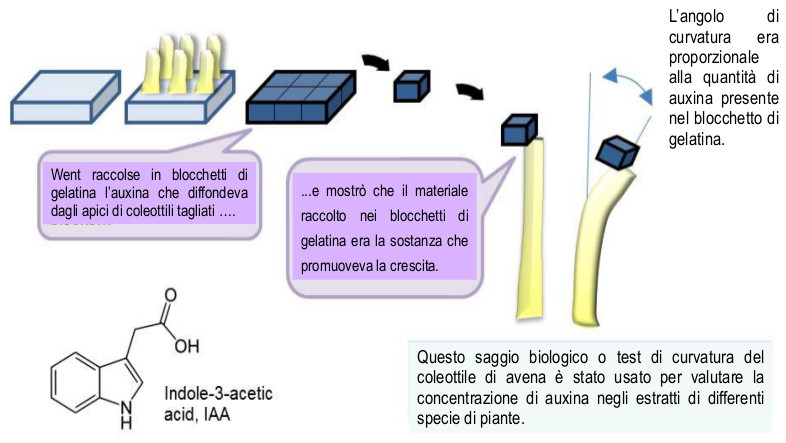
\includegraphics[scale=0.4]{immagini/coleottile.jpg}
\end{figure}
Se siamo in ombra, l'auxina si dispone su tutto il coleottile e non si ha curvatura.

L'auxina è un acido indolico-3 acetico, in cui il gruppo indolico è responsabile dell'attività dell'auxina\footnote{Esistono altre forme di auxina, tutte caratterizzate dalla presenza dell'anello nella struttura}. È una molecola anfipatica.

La distanza tra il gruppo acido e l'azoto di 0,5 nm si pensa sia indicatore della caratteristica che ha l'auxina. La maggior parte sono erbicidi. L'auxina in grande quantità ha un effetto negativo sulla crescita della pianta perchè promuove la produzione di elevati livelli di etilene, che ha efetto erbicida promuovendo la senescenza accelerata, quindi la morte della pianta.

Gli ormoni sono di solito coniugati per essere resi intattivi e trasportabili nei vari tessuti- al sitoo di destinaizone abbiamo enzimi che deconiugano gli ormoni per farli agire. 
\subsection{Biosintesi dell'auxina}
A partire dal triptofano si hanno varie vie di sintesi, di cui la più famosa è la IPA: transaminazione del triptofano con produzione di \emph{acido indol-3 piruvico} (IPA), che viene decarbossilato a indolo 3-acetaldeide (IAld) dall'IPA decarbossilasi, ridotto poi a indolo 3-acido acetico(IAA) dall'enzima IAld-deidrgenasi
\begin{figure}[H]
\centering
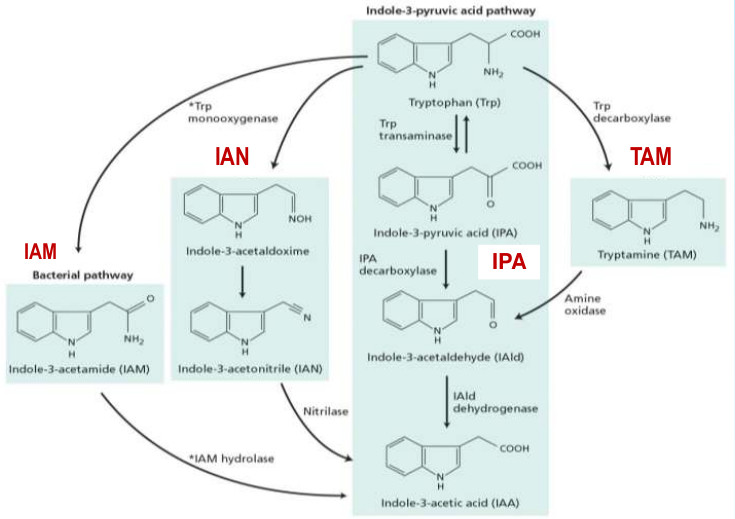
\includegraphics[scale=0.4]{immagini/biosintesi.jpg}
\caption{Vie di biosintesi dell'auxina}
\end{figure}

Nei mutanti di mais \emph{orange pericarp}, alcune cariossidi sono arancioni perchè non in grado di sintetizzare triptofano. Queste cariossidi erano comunque ricche di auxina e ciò ha permesso di identificare un'altra via di produzione dell'auxina, indipendente dal Trp.

L'auxina è sintetizzata in tutti i meristemi, anche se in diverse quantità: nel meristema apicale ne abbiamo di più rispetto al meristema apicale. Questo perchè questi due tessuti sono sensibili diversamente all'auxina.
Per identificarla nel SAM di una foglia apicale, si usa un gene reporter GUS duso ad un promotore della pianta che risponde all'auxina libera nel tessuto. L'auxina, nelle zone che attraversa, promuove il differenziamento vascolare.

L'esistenza di vie multiple per la sintesi dell'ormone
ha un vantaggio evoluzionistico per cui la pianta non
corre mai il rischio di trovarsi priva di auxina; ciò
rimarca ancora una volta il ruolo essenziale di
questo ormone nella vita della pianta stessa.

\subsection{Localizzazione dell'auxina}
Sebbene IAA libero sia la forma biologicamente attiva dell’ormone presente nei meristemi apicali ed in
giovani foglie, gran parte si trova coniugata con proteine e peptidi (coniugati ad alto PM) o esterificata con zuccheri, in particolare glucosio (coniugati a basso PM), con produzione di IAA-glucosio, che è il coniugato più presente, oppure con ammidi, conugati che sono forme inattive dell'ormone.
 \emph{I coniugati
sono biologicamente inattivi}. La loro formazione può essere collegata al trasporto ed alla conservazione
dell’ormone. I coniugati, a seguito di idrolisi enzimatica, rilasciano IAA libero.

L'\emph{auxina coniugato sintetasi} è un gruppo di enzimi che coniuga l'auxina con ammidi. Mutanti per sovraespressione di sintetasi GH3-13 riducono l'accrescimento della pianta. Questi enzimi sono regolati con meccanismo a feedback negativo dai livelli di auxina stessa.

\paragraph{Catabolismo ossidativo dell'auxina} In vitro IAA è facilmente degradato in soluzione acquosa da luce UV e visibile in presenza di pigmenti
fotosensibilizzanti come la riboflavina. Non è chiaro il significato di tale fotoossidazione in vivo. Inoltre IAA
è ossidato enzimaticamente dalla IAA-ossidasi (perossidasi) a 3-idrossimetilossindolo; sono state
scoperte anche altre vie di degradazione dell’ormone, delle quali però si hanno conoscenze limitate.
\subsection{Trasporto di auxina}
L'auxina viene trasportata nel floema in direzione basipeta\footnote{dall'alto verso il basso} (verso i vasi), con un sistema che ne comporta il \emph{trasporto polare}: a breve distanza, l'auxina viene trasportata in direzione basipeta per quanto riguarda le parti verdi della pianta, e in direzione acropeta\footnote{procede verso il basso allontanandosi dal suolo} se avviene a livello della radice, poi torna leggermente verso l'alto. Basipeta ed acropeta sono trasporti verso il basso, ma se il trasporto avviene sopra il suolo è detto vasipeta, se sotto il suolo è detto acropeta.

Se prendiamo un apice di coleottile e lo recidiamo, ponendolo tra due blocchetti contenenti uno auxina e l'altro senza, si nota che l'auxina si muove verso il basso. Se ruotiamo il coleottile e lo mettiamo nelle condizioni precedenti (auxina sopra e no auxina sotto) il trasporto di auxina non avviene. Il trasporto va quindi vero il basso del coleottile, non verso il basso in generale (quindi non si spiega per gravità).

\paragraph{Modello di diffusione chemiosmotica} L'apoplasto ha un pH intorno a 5:  l'auxina, che ha una pK di 4.75, si trova in forma indissociata (solo il 25 ì\% è dissociata): questa forma è diffusibile perchè si crea un gradiente di concentrazione, visto che nel citoplasma il pH è 7 e l'auxina si dissocia. Esiste alla base della cellula un sistema di trasorto che estrude la forma dissociata di nuovo verso l'apoplasto, dove si riprotonerà. Questo dirige il flusso in una direzione precisa grazie ai carrier dell'auxina che si trovano sul lato basale della cellula.
\begin{figure}[H]
\centering
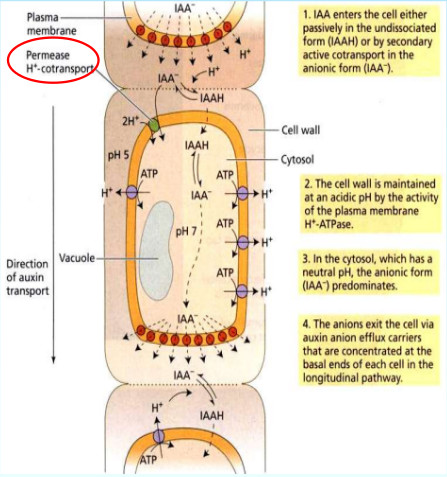
\includegraphics[scale=0.4]{immagini/chemio.jpg}
\caption{Modello di diffusione chemiosmotica}
\end{figure}

Ci sono 3 gruppi di proteine che mediano il passaggio di auxina: 
\begin{enumerate}
\item{ABCB transporters : trasporto di auxina}
\item{AUX 1 e LAX : trasportatori di influsso, mediano l'ingresso di IAA- nel citoplasma}
\item{Proteine PIN : trasportatori di efflusso, si trovano in varie localizzazioni a seconda delle necessità della pianta di localizzare in alcuni punti l'auxina}
\end{enumerate}

Le proteine PIN sono state identificate nei mutanti Arabidopsis in cui l'insufficienza di auxina provoca un'infiorescenza apicale a forma di spillo: PIN1 è uno dei carrier di efflusso per l'auxina posto in posizione basale, guidando la direzionalità del trasporto. È stata trovata anche a livello dell'apice meristematico.

(16.03.2015)

Il trasporto polare dell'auxina è fondamentale in risposte che riguardano sviluppo, accrescimento e morfogenesi. I trasportatori ABCB coadiuvano l'azione delle PIN. Le PIN si trovano anche all'interno del citoplasma e sono coinvolte nella traslocazione dell'auxina nel RE. Ciclo di inserimento delle PIN nella membrana plasmatica a partire dal pool endosomico. Si pensa che l'auxina abbia un ruolo di localizzazione a feedback positivo delle proteine PIN sulla membrana.

\section{Vie di trasduzione dell'auxina : percezione e signaling}
ABP1 è un recettore proteico che determina l'attività di estrusione dei protoni, promuovendo la sintesi di pompe di membrana o attivando quelle vecchie.
La pompa protonica
estrude protoni nello spazio infraparete indebolendo i legami della matrice.
C'è un recettore citosolico solubile TIR1, che a seguito dei legami con l'ormone lega una proteina bersaglio, destinandola all'ubiquitinazione nel proteasoma. È una proteina F-box solubile facente parte del complesso $SCF^{TIR1}$. In generale i complessi SCF
catalizzano il legame covalente dell’ubiquitina a proteine che sono così \emph{segnalate} per la proteolisi.

\paragraph{ABP1}
Sembra legato alla regolazione di risposte auxiniche mediate da trasporto ionico attraverso la membrana; TIR1 è invece legato all'attività di trasfezione dell'auxina. Al legame di auxina con ABP1 si attiva una via di trasduzione che porta alla sintesi e alla localizzazione di pompe protoniche ATPasiche sulla membrana: attivate, promuovono la traslocazione di protoni verso l'apoplasto, mediando le risposte dell'auxina che portano all' acidificazione dell'apoplasto \lfreccia apertura di canali K, il K entra all'interno della cellula insieme ad acqua. L'acidificazione dell'apoplasto porta ad eventi che determinano l'\emph{allentamento della matrice}, costituita da componenti legati da ponti a idrogeno, i quali vengono inibiti dall'acidificazione e dall'attivazione di enzimi che lavorano a pH acido e compromettono questi legami.
\begin{figure}[H]
\centering
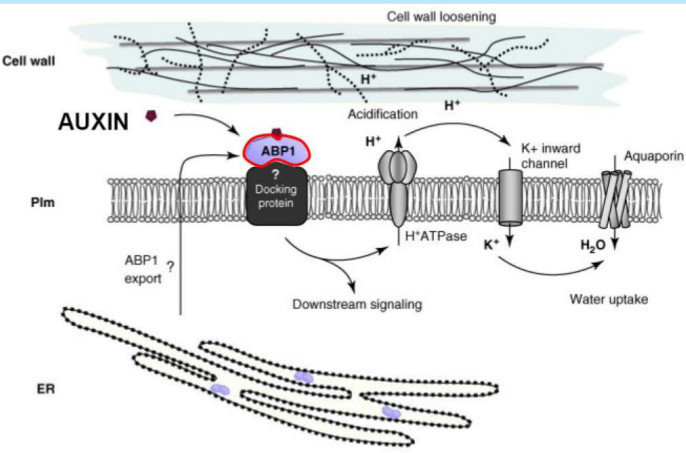
\includegraphics[scale=0.4]{immagini/aux.jpg}
\caption{Azione di ABP1}
\end{figure}

In assenza di auxina, i geni indotti dal segnale auxinico sono repressi alla presenza di AUX/IAA, una proteina repressore.

I complessi $SCF^{TIR1}$ legano l'ubiquitina a proteine bersaglio  che saranno poi degradate: il bersaglio in questo caso è AUX/IAA, proteina repressore della risposta auxinica. È una famiglia di proteine nucleari. Il repressore è omologo nella sequenza alle proteine ARF, che sono dei regolatori positivi della trascrizione genica. AUX/IAA si lega, una volta percepita l'auxina, ad ARF, favorendo la trascrizione dei geni. Il legame di ARF agli elementi che rispondono all'auxina è impedito perchè questi ultimi, in assenza di auxina, si trovano legati alle sequenze geniche del repressore. Quando viene  percepito il segnale auxinico, vengono degradadt TIR1 e AUXIAA: ARF diventa omodimero ARF ARF e si lega alle sequenze geniche, attivando la trascrizione dei geni legati al'auxina.

Quindi, ARF si trova di norma complessato con AUX/IAA: quando arriva il segnale auxinico, AUX/IAA viene degradata ed ARF va ad attivare la trascrizione dei geni auxinici. Ci sono geni precoci e geni tardivi. 

I geni precoci sono AUX/IAA e SAUR e GH3.

I geni tardivi sono quelli che mediano risposte auxiniche a diversi tipi di stress.

\section{Effetti fisiologici dell'auxina}
L'auxina regola moltissime funzioni a livello della pianta: controlla una serie di funzioni fondamentali per sviluppo, formazione e riproduzione della pianta:
\begin{itemize}

\item{Nella radice mantiene il meristema apicale attivo e il centro quiescente tale, in modo da costituire un nucleo di cellule che, man a mano che si allontanano da esso, si differenziano in cellule radicali}
\item{Determina la vascolarizzazione dei vari tessut}
\item{A livello del meristema del germoglo induce la formazione di foglie e fiori}
\end{itemize}
Quando una cellula sotto effetto dell'auxina vede un aumento di dimensioni del vacuolo a causa di un richiamo di acqua, la parete, per effetto dell'auxina, si allenta (grazie ad ABP1) e risponde distendendosi all'aumentata pressione di turgore.

(manca un pezzo, lo ha preso fra)\todo{Chiedi a Fra}

Se forniamo a tessuti escissi auxina in concentrazioni crescenti, osserviamo che all'aumentare della concentrazione c'è un progressivo aumento della crescita fino ad un massimo, oltre il quale ulteriori aggiunte di auxina fanno addirittura contrarre la cellule (si pensa sia dovuto all'effetto dell'auxina sull'etilene, che inibisce la crescita cellulare). A seconda dei tessuti si ha una sensibilità diversa all'auxina: la radice è più sensibile del fusto.

Come fa l'auxina a promuovere la distensione?

Si è divisa la crescita in risposta iniziale e risposta prolungata: nella risposta iniziale, utilizzando inibitori di sintesi ATP e della pompa protonica, non si aveva crescita. Anche non fornendo auxina ma acidificando il pH si ha lo stesso effetto della somministrazione dell'auxina.

La risposta prolungata non dipende dal pH ma richiede che siano presenti saccarosio o osmoliti di diversa natura che, una volta entrati nella cellula, la mantengano distesa mantenendo un alto livello di turgore. Si ha anche sintesi di componenti di membrana che servono per sostenere la distensione. Parallelamente alla crescita si osserva un'estrusione di protoni.

\subsection{Teoria della crescita acida}
L'effetto dell'auxina porta alla secrezione di protoni nell'apoplasto, quindi nella matrice della parete, attraverso sintesi di nuove pompe di membrana: si ha la rottura di legami ad H  grazie all'inacidificazione o all'attività di enzimi. Questa rottura porta all'allentamento della parete che, a seguito dell'aumento del turgore, fa si che la cellula possa distendersi.

Ci sono 2 effetti dell estrusione di H+:
\begin{enumerate}
\item{Allentamento del network della parete}
\item{Degradazione di componenti della parete per effetto delle \textbf{espansine}, proteine con attività enzimatica che richede pH acido}
\end{enumerate}

Un coleottile viene congelato e scongelato, l'epidermide viene erasa e trattata a calore per inattivare attività enzimatiche, poi incubata e soggetta ad una tensione misurata grazie ad un grave applicato al tessuto: ciò permette di misurare la distensione del tessuto. Se nel mezzo di incubazione mettiamo un'estratto dei coleottili escissi, osserviamo una distensione del tessuto: nell'estratto di questo tessuto sono presenti sostanze che hanno bisogno di mantenersi attive.

\subsection{Modello di Cholodny-Went}
Ipotizza che la percezione di uno stimolo luminoso direzionale provochi il trasporto laterale di auxina, causando crescita differenziata. L'auxina si mette sul lato in ombra. Si ha una ridistribuzione del trasporto mediato da PIN3. 

\paragraph{Fototropismo}
Esperimenti su mutanti di Arabidopsis non rispondenti all’illuminazione unilaterale, hanno evidenziato una
mutazione del gene \emph{phot1} codificante per una proteina detta \emph{fototropina}. La fototropina è una
serina/treonina chinasi di membrana con PM 116 kDa. La proteina presenta attività chinasica nella
porzione COOH-terminale, mentre in quella NH2-terminale possiede i siti di legame al flavin
mononucleotide (FMN). A seguito dell’illuminazione con luce blu assorbita dal FMN la fototropina si
autofosforila.
L’autofosforilazione porta al distacco della fototropina dal plasmalemma e alla sua interazione con i
trasportatori di auxina. È stato dimostrato in coleottili che a seguito della illuminazione unilaterale si forma
un gradiente di autofosforilazione della fototropina che sarebbe responsabile del movimento laterale di
auxina.
\begin{figure}[H]
\centering
\includegraphics[scale=0.4]{immagini/fototropina.jpg}
\caption{Fototropismo}
\end{figure}

 
\paragraph{Gravitropismo}
Quando il seme viene ruotato di 90 gradi, si ha un riorientamento della crescita ancora in direzione della luce, mentre la radicicola posta in posizione orizzontale si orienta crescendo verso il basso. Nella radice, l'auxina sta a livello dell'apice radicale, in particolare nel centro quiescente, quando viene posta in posizione orizzontale: l'auxina si distribuisce sul lato inferiore della radice; quando la trattiamo con un inibitore del trasporto auxinico, si ha mancata distribuzione di auxina e mancata risposta gravitopica.

Nella radice, dove si ha accumulo di auxina, si ha una \emph{diminuzione} della crescita. 

\paragraph{}
La percezione della gravità nella radice è dovuta alla \emph{cuffia}: se viene rimossa, non si ha nessuna risposta gravitropica. Lo stimolo della gravità è dato dagli statoliti che si trovano nelle cellule della cuffia:
\begin{itemize}
\item{ Quando la radice è orientata in verticale, gli statoliti si
ridistribuiscono su tutto il RE, esercitando una pressione
uniforme sul reticolo}
\item{ Quando la radice è orientata orizzontalmente, la pressione
esercitata sul RE dagli statoliti appartenenti agli statociti dei
due lati della radice è diseguale}
\end{itemize}
La crescita geotropica causa variazioni di pH nell'apoplasto, dovute ad un aumento dell'attività della pompa protonica, determinando la distensione sul lato verso l'alto della radicicola e un'inibizione della distensione sul lato inferiore.

Il ruolo principale nella crescita geotropica nella radice lo ha \emph{PIN3}, coinvolto nel trasporto dalla zona centrale della radice verso il basso. Nel caso in cui la radice venga riorientata, si dispone sul lato inferiore promuovendo la traslocazione dell'auxina.

\subsection{Effetti dell'auxina sullo sviluppo}
L'auxina è un \emph{morfogeno} nell'\emph{embriogenesi}: si osserva una precisa disposizione dei traslocatori che determina una distribuzione polare dell'auxina già ai primi stadi dell'embriogenesi. L'auxina si concentra nelle zone in cui si formeranno i cotiledoni: si ha un trasporto vasipeto dell'auxina lungo le linee di distribuzione che daranno luogo ai fasci vascolari della pianta.
\begin{figure}[H]
\centering
\includegraphics[scale=0.4]{immagini/morfo.jpg}
\caption{Auxina come morfogeno per l'embriogenesi}
\end{figure}
È anche un morfogeno per lo \emph{sviluppo della radice}: i mutanti \emph{yucca} per una proteina di catabolismo dell'auxina mancano di radici. I mutanti PIN invece vedono perdita di funzione dei trasportatori dell'auxina: si ha completa assenza di forma dell'embrione.

È anche un morfogeno nella \emph{differenziazione dello xilema}: l’auxina
forma un gradiente di
concentrazione
diretto
internamente dal cambio cribro
vascolare verso il floema ed
esternamente verso lo xilema
che si stanno sviluppando.
\begin{figure}[H]
\centering
\includegraphics[scale=0.4]{immagini/morf.jpg}
\caption{Auxina come morfogeno nello xilema}
\end{figure}

È un morfogeno a livello dell'\emph{apice radicale}: dove c'è minor auxina c'è maggior distensione. C'è una zona indifferenziata che si accresce per distensione. Le cellule vicine all'apice sono soggette ad un livello intermedio di auxina: si dividono molto, ma differenziano poco. Le cellule del centro quiescente rimangono tali a causa degli alti livelli di auxina. 

I massimi di auxina sono importanti per il differenziamento di vari organi nella pianta: ad esempio nell'induzione del differenziamento del fiore. Trattando mutanti Pin1 diArabidopsis con alte concentrazioni di auxina in una parte dell'apice vegetativo, si osserva la formazione di un primordio fogliare con sviluppo di infiorescenza. La distribuzione di auxina in punte di massimo nel meristema apicale porta alla formazione di abbozzi fogliari e di infiorescenze.

L'auxina promuove anche la formazione di radici laterali: si ha accrescimento del periciclo che determinerà l'abbozzo della radice: si ha in corrispondeza di un massimo della distribuzione di auxina.

Altro ruolo si ha nella \emph{dispersione del seme}: in Arabidopsis si ha una silica e l'apertura avviene in due zone in corrispondenza di due minimi di concentrazione di auxina.

\paragraph{Dominanza apicale} la gemma apicale controlla lo sviluppo delle gemme sottostanti laterali, inibedole. Se rimossa, si sviluppano le gemme sottostanti. La responsabile è l'auxina prodotta dalla gemma apicale. Si riteneva che l'auxina si spostasse all'interno di queste gemme: in realtà l'auxina non penetra nelle gemme laterali, ma esercita una funzione a distanza a livello dello xilema, del fascio vascolare, che raggiunge la gemma.

\paragraph{}
L'auxina promuove lo sviluppo dei frutti: i semi stessi, producendo auxina, inducono la formazione di espansione del ricettacolo, ottenendo un falso frutto.

(manca una lezione, c'è l'audio)

(23.03.2015)
 
\chapter{Gibberelline}

Le gibberelline si muovono nella pianta anche con il trasporto a lunga distanza, ma non sappiamo se ciò avviene davvero nella pianta.

Quelle prodotte dal fiore maschile servono per lo sviluppo dell'intero fiore, quindi devono essere traslocati nei tessuti adiacenti, ma è un trasporto a breve distanza.

\section{Trasduzione del segnale}
In Arabidopsis sono stati usati esperimenti della crescita del fusto della pianta: un \emph{wt} trattato con gibberelline ha un fusto più lungo. Un mutante che ha meno gibberelline, se somministrate risponde e abbiamo una pianta normale. Un mutante che non risponde al trattamento con gibberelline esogene non dà risposta in termini di accrescimento.
\begin{figure}[H]
\centering
\includegraphics[scale=0.4]{immagini/gib.jpg}
\caption{Risposte al GA in Arabidopsis}
\end{figure}

Altri mutanti interessanti sono i mutanti \emph{slender}: hanno la stessa crescita del fusto sia che si tratti con GA che non si tratti. I livelli di crescita sono quindi troppo elevati: si ha la mancata riduzione dell'inibitore della trascrizione indotta dalle gibberelline. 

Il mutante insensibile alla gibberellina è risultato essere coinvolto nella percezione del segnale ed ha permesso di identificare il recettore per le gibberelline, GID. Questo recettore ci ha permesso di capire quando la proteina è sovraespressa. Aumentare il livello delle gibberelline nel mutante in cui GID è sovraespresso determina un ulteriore aumento dell'accrescimento.

Questa proteina GID funziona quindi da recettore per le gibberelline: in Arabidopsis 3 geni per GID, A B e C, che possono essere espressi contemporaneamente. Se tutti e tre sono mutati, il mutante triplo non cresce. Se ne mutano uno o due invece si ha crescita.

Il mutante privo di GID è insensibile alle gibberelline.

\paragraph{GID} 
Recettore solubile, nucleare, che presenta all'estremità ammino-terminale una gibberellina, LID, che si ripiega sulla tasca. La proteina DELLA, al momento in cui la gibberellina si lega al recettore, subisce una modificazione: la gibberellina si lega al core grazie a molecole di acqua, si ha modificazione conformazionale che determina la chiusura del coperchio. A questo punto DELLA\footnote{Nella mutazione slander non è funzionale} si trova legata al complesso recettore-gibberellina: la proteina ha un dominio GRAS carbossi terminale e una volta che si è legata al recettore cambia conformazione \lfreccia ciò determina suscettibilità ad un complesso SCF che, legandosi al dominio Gras, subisce l'ubiquitinazione: DELLA viene degradata e si chiude il suo effetto inibitorio sulla trascrizione.


DELLA si lega ad un fattore di trascrizione impedendo proprio la trascrizione: quando viene degradata, la trascrizione può avere luogo e si osserva la crescita dello stelo.

\subsection{Cereali}
La cariosside è un frutto secco indeiscente: embrione + tessuto di riserva. Il rivestimento di frutto e seme sono fusi: il pericarpo è fuso con il testa (rivestimento del seme). All'interno c'è un tessuto che si chiama \emph{aleurone}, che produce la crusca. Al di sotto di pericarpo e testa c'è l'\emph{endosperma}, tessuto di riserva che può essere amilaceo (contiene amido) oppure morto, perchè c'è un accumulo elevatissimo di amido in queste cellule in grado di provocare la rottura della membrana. All'esterno dell'endosperma amilaceo c'è l'aleurone, ovvero fra endosperma e testa-pericarpo.
 
 È l'embrione che contiene le gibberelline e all'inizio della germinazione rilascia questi ormoni: vengono percepiti dallo strato aleuronico. Il rilasco di gibberelline nello sperma promuove l'idrolisi delle riserve contenute nell'endorperma amilaceo (amido, proteine di riserva ecc). Le cellule aleuroniche sono in grado di percepire il segnale. Ci sono nell'aleurone dei vacuoli in cui sono conservate grandi quantità di un tipo particolare di proteine di riserva: esse vengono idrolizzate quando arrivano le gibberelline e vengono usate per nuove sintesi, come proteasi, $\alpha$-amilasi (degradazione amido).

La gibberellina promuove la sintesi di \emph{$\alpha$-amilasi}; prima della sintesi di mRNA si osservano alti livelli di GAMYB, un fattore di trascrizione che risponde alla gibberellina. Una delle evidenze è un aumento dei livelli citoplasmatici di Ca: è uno degli effetti delle gibberelline. All'interno del nucleo, la gibberellina di lega al suo recettore. La proteina DELLA viene degradata ed era associata a GAMYB: il promotore di GAMYB è ora libero e si ha la sintesi di GAMYB, che si lega alla sequenza GARE e promuove la trascrizione per la $\alpha$-amilasi. I livelli di Ca avevano la funzione di mediare la secrezione dell'enzima al di fuori dell'aleurone in vescicole.

\section{Effetti fisiologici}
Le gibberelline hanno ruoli in varie fasi dello sviluppo della pianta, soprattutto nella germinazione dei semi. Il seme si dice dormiente, ha attività metaboliche ridotte durante la quiescenza. L'acido abscissico ABA mantiene questo stato: per rompere la dormienza si osserva una diminuzione dei livelli di ABA ed elevati livelli di GA. A questo punto la pianta inizia a crescere, e la crescita è sempre promossa dalle gibberelline.

\subsection{Effetti sull'allungamento del fusto}
Nella barbabietola, servono giornate con lungo periodo di illuminazione. La gibberellina però, a prescindere dal tipo di illuminazione (breve o prolungata), promuove la crescita della pianta. 

Nelle Brassicacee (Arabidopsis), se forniamo GA si osserva anche in brevi fotoperiodi un effetto formidabile di distensione del fusto. In queste piante, fornendo GA esogena si osserva nel meristema apicale una distensione, dovuta ad aumento di attività mitotica.

Le GA agiscono anche a livello del \emph{meristema intercalare del fusto}: si ha la distensione delle cellule di questo tessuto. 

Si ha anche un effetto sull'allungamento dei MT corticali: la distensione è favorita dalla separazione di questi MT e da una classe di enzimi, XET, delle xiloglucano endo-transglicosidasi che agiscono sulle emicellulose della parete staccando frammenti terminali e riarrangiandoli su altre microfibrille di cellulosa, permettendone l'allungamento e la distensione.

In caso di rapido aumento dell'acqua nell'ambiente, come un'inondazione,  le GA aumentano la loro espresisone affichè il fusto si accresca rapidamente e la parte più apicale rimanga emersa. Questo però comporta un richiamo di sostanze per la crescita vegetativa a scapito del seme.

In piante mutate per accumulo di proteina DELLA, si ovvia a questo problema impedendo alla pianta di crescere anche se viene sommersa; se l'inondazione è per breve periodo, la pianta sopravvive.

Il riso transgenico Sub1A è un esempio di questo comportamento.

\subsection{Effetti sul passaggio dalla fase giovanile a quella adulta}
Le GA sono coinvolte in questo passaggio da fase vegetativa a fase rispoduttiva: il trattamento con GA può sovrascrivere il programma di passaggio di fase.

Nello sviluppo dei fiori, una mutazione del gene GAMYB porta a mancato sviluppo di antere \lfreccia sterilità

\subsection{Effetti sulla maturazione del frutto}
Le GA promuovono la crescita dei frutti: se forniamo auxine insieme a GB in fiori non impollinati, si ha lo sviluppo e la crescita dei frutti.

\subsection{Germinazione dell'orzo}
Per fare la birra.

Un buon malto si ha quando la quantità di amido degradato è tale da non venire utilizzata dall'embrione ma da servire per lo sviluppo (quindi abbastanza ma non troppo): nel processo di maltazione le GA vengono fornite per accelerare il processo.

\chapter{Citochinine}
La prima citochinina (CK) fu scoperta mentre
si stavano cercando sostanze che fossero in
grado di stimolare la crescita per divisione in
colture di tessuti vegetali.

Esse infatti promuovono la divisione cellulare. Trattando cellule totipotenti con \emph{chinetina}, dopo la divisione cellulare si aveva anche crescita del fusto. Si trattava comunque di un composto non naturale, ma di un
prodotto di decomposizione del DNA in cui il deossiribosio
dell’adenosina è convertito in furano che è distaccato dalla posizione
9 ed attaccato in posizione 6 dell’adenina.
\begin{figure}[H]
\centering
\includegraphics[scale=0.4]{immagini/chinetina.jpg}
\caption{Struttura della chinetina}
\end{figure}

Trattandole con auxina invece si osservava lo sviluppo di radici. Se le concentrazioni dei due ormoni venivano mantenute uguali, si aveva sviluppo di calli. Auxina e citochinine sono ormoni utilizzati in vitro per riprodurre cloni di piante da cui il tessuto trattato è stato espiantato.
    
\section{Struttura delle citochinine}

Nel 1973 Letham isolò la prima CK naturale da estratti di endospermi immaturi di mais e la chiamò zeatina. La \textbf{zeatina}\footnote{in particolare l'isomero TRANS} è stata individuata in Zea Mays: la sua catena laterale presenta un doppio legame, perciò può esistere nelle configurazioni \emph{cis} e \emph{trans}. Essa è la CK prevalente. Altre due CK sono la \textbf{diidrozeatina} e la \textbf{isopenteniladenina}.
\begin{figure}[H]
\centering
\includegraphics[scale=.35]{immagini/CK.jpg}
\caption{Struttura delle varie citochinine}
\end{figure}
Le citochinine si trovano anche legate al tRNA in corrispondenza di determinati aa: si pensa che possano essere forme di \emph{conservazione} delle citochinine o che derivano dalla degradazione del tRNA, poichè quelle biologicamente attive sono quelle in forma libera.

\section{Biosintesi delle citochinine}
I geni per la sintesi delle citochinine sono stati scoperti grazie all'induzione del tumore del colletto da \emph{Agrobacterium tumefaciens}: il plasmide T contiene T-DNA che contiene geni per i fattori patogenetici e viene utilizzato per la produzione di piante trasngeniche monocotiledoni. La scoperta di questo meccanismo di infezione ha permesso il grande sviluppo di piante trasngeniche. L'agrobacterium induce la sintesi di auxine e citochinine! 

Il gene \emph{IPT} del T-DNA codifica per l’enzima \emph{isopentenil transferasi} (IPT). Inoltre il T-DNA (geni tmr, tumor) contiene due geni codificanti enzimi della biosintesi di auxine (da triptofano ad IAA). I tre geni suddetti
sono chiamati fito-oncogeni poiché possono indurre tumori nelle piante. Essendo i promotori di questi
geni presenti solo nelle piante, non sono espressi nei batteri. La loro trascrizione nelle piante porta alla
produzione di auxina, CK e opine (composti contenenti C e N per la nutrizione dei batteri, ma non delle
piante).

\subsection{Biosintesi della trans-zeatina}

I substrati preferenziali di IPT sono ATP o ADP e DMAPP (dimetilallil difosfato) che deriva dalla biosintesi del MEP (metileritriolo fosfato).
I precursori delle CK biologicamente attive, iPDP o iPTP, possono essere idrossilati dalla \emph{citocromo P450
monoossigenasi} (CYP735A) per produrre tZDP o tZTP, precursori di tZ. Perciò l’attività di CYP735A contribuisce all’
abbondanza relativa di iP oppure di tZ.

\begin{figure}[H]
\centering
\includegraphics[scale=0.4]{immagini/biosintesi2.jpg}
\caption{Biosintesi della trans-zeatina}
\end{figure}

La perdita del ribosio fosfato avviene grazie all'azione dell'enzima \emph{CK riboside 5'-monofosfato-fosforibosio idrolasi}, che è stato scoperto analizzando il mutante di riso log, caratterizzato da meristema apicale difettoso e incapace di funzionare.
\begin{figure}[H]
\centering
\includegraphics[scale=0.4]{immagini/bio3.jpg}
\caption{Azione dell'enzima CK riboside 5'-monofosfato-fosforibosio idrolasi}
\end{figure}

\subsection{Catabolismo}
Il catabolismo dell'inattivazione di questi ormoni avviene per \emph{coniugazione} o \emph{degradazione}. La degradazione è un'inattivazione irreversibile e comporta l'ossidazione dell'ormone da parte della \emph{CK ossidasi}, distribuita in tutti i tessuti della pianta, ma incapace di ossidare le forme coniugate delle CKs. Le forme coniugate si ritrovano spesso con il glucosio.

(25.03.2015)

\section{Trasporto delle citochinine nella pianta}
Sono traslocate a lunga distanza: sia nel succo floematico che nella linfa grezza dello xilema, ma una distribuzione diversa; nel floema ci sono più forme coniugate (isopenteniladelina e cis-pentatina), mente nello xilmena alti livelli di ribosil-trans-zeatina, sintetizzata ad alte concentrazioni nella radice, perchè nelle radici troviamo alti livelli di un enzima che converte in trans-zeatina il precursore della isopenteniladelina.

Il mutante che risulta dalla quadrupla mutazione (ipt1;3;5;7) vede una crescita ridotta e un ridotto accrescimento secondario della pianta. Praticando un innesto con il fusto o con la radice del wild-type, recuperiamo il fenotipo: ciò significa che:
\begin{enumerate}
\item{Le CKs sono trasportate a lunga distanza a partire sia dal fusto che dalla radice}
\item{Le CKs sono essenziali nella differenziazione del cambio}
\end{enumerate}

Trattando specie con una forte dominanza apicale, l'induzione del gene IPT promuove la crescita di gemme laterali, ma solo a livello del nodo indotto. Ciò significa che le citochinine sintetizzate agiscono solo localmente e con un segnale paracrino. Come vengano spostate localmente nel tessuto in cui sono prodotte non si sa: probabilmente c'è un trasportatore, che però non è specifico per le citochinine.

\section{Trasduzione del segnale}
È dipendente da un sistema \emph{fosforelay} in cui anzichè utilizzare una cascata di chinasi e fosforilasi per il trasferimento di gruppi Pi, vede i gruppi Pi trasferiti direttamente da un elemento all'altro del sistema, fino ad attivare i regolatori di risposta.

Questo sistema è omologo a quello dei batteri: abbiamo un sensore per eventi ambientali esterni che risponde attraverso l'autofosforilazione di un residuo di Hys che si trova nella parte sensoria della molecola; trasferisce il Pi su un dominio Asp del regolatore di risposta che viene attivato: nei batteri ciò attiva la trascrizione.

Nelle piante questo componente D del regolatore di risposta si associa al sensore ibrido istidina chinasi, mentre un'altra copia resta associata al regolatore. Questo tipo di percezione del segnale è stato individuato nelle citochine e porta all'attivazione della trascrizione. Il trasferimento del Pi al dominio ricevente D avviene razie al componente HPt (istidina fosfotransferasi).
\begin{figure}[H]
\centering
\includegraphics[scale=0.4]{immagini/sensore.jpg}
\caption{Sistema fosforelay di segnale a due componenti}
\end{figure}

Il sensore ibrido ha una componente che attraversa la membrana e attraverso questo dominio riceve il segnale della citochinina \lfreccia fosforilazione Hys \lfreccia fosforilazione Asp.

L'istidina fosfotrasferasi raggiunge la membrana del nucleo, determinando l'attivazione dei regolatori di risposta:  trasferendo un gruppo fosforico al dominio ricevente D del regolatore di risposta, ne altera
l’attività. In definitiva HPt funziona come un relay azionato da gruppi fosforici che va ad attivare il regolatore di
risposta.

\subsection{Fosforelay in Arabidopsis}
In Arabidospis troviamo 3 recettori per le CHs: AHK2, AHK3 ad AHK4. I recettori di CKs sono di natura proteica, formati da chinasi ibride e presenti come componenti transmembrana. Tutti i
recettori di CKs hanno in comune un dominio *CHASE extracellulare che lega la CK. I tre recettori hanno distinte affinità
per diversi tipi di CKs, suggerendo funzioni distinte nella pianta.

Le piante che presentano mutazioni triple nel recettore della citochinine vivono comunque: ciò suggerisce che ci siano altre proteine analoghe a questi recettori. Tra queste vi sono recettori per la percezione del segnale etilenico, anche se non è chiaro che agiscano da veri recettori del segnale etilenico. 

L’istidina fosfotransferasi (AHP) funziona da navetta tra il citoplasma ed il nucleo. 
La HPt viene fosforilata da AHK, ricevendo il gruppo fosforico dal recettore AHK, e quindi diffonde dal
citoplasma nel nucleo, dove trasferirà il fosfato ad un Asp del dominio ricevente del regolatore di
risposta (ARR).

Gli ultimi componenti del sistema di fosforelay sono i \emph{regolatori di risposta}. Ce ne sono di 3 tipo
\begin{enumerate} 
\item{Tipo B, regolatore positivo} 
\item{Tipi A e C, che sono regolatori negativi}
\end{enumerate}

Un \textbf{regolatore di tipo B} ha il dominio ricevente all'estremità N-terminale, e il dominio di output, che lega il DNA, sta più verso l'estremità C-terminale. La sua sovraespressione rende i tessuti più sensibili alle CKs. Questi ARR di tipo B sono parzialmente ridondanti: mutanti singoli sono sempre sensibili alle CKs, mutanti doppi e tripli invece provocano risposte danneggiate.

Un \textbf{regolatore di tipo A} è rapidamente indotto da CKs. Questi regolatori presentano un solo dominio ricevente contenente aspartato (D). Sono dei regolatori negativi del signaling di CKs: infatti sia che vengono fornite o meno citochinine, l'espressione della luciferasi è ridotta. Questi regolatori competono con i B per l'aquisizione dei gruppi Pi dall'istidina fosfotrasferasi.

I \textbf{regolatori di tipo C} non hanno domini per il legame al DNA, ma somigliano al sensore istidina chinasi, anche se hanno attività fosfatasica: il loro effetto negativo è dovuto alla rimozione di gruppi Pi. Essi non sono indotti dalle CKs.

Questi regolatori quindi, seppur con diverse funzioni, controllerebbero l'espressione dei geni bersaglio.
\begin{figure}[H]
\centering
\includegraphics[scale=0.4]{immagini/ARR.jpg}
\caption{Funzioni dei 3 tipi di ARRs}
\end{figure}

\section{Funzioni}
Mantenimeno dell'attività di divisioni dei meristemi apicale e radicale; sono coinvolte nella determinazione della struttura della pianta insieme alle auxine proprio perchè mantengono attivo il meristema apicale. 

Mantenimeno dell'integrità strutturale; attività morfogenetiche delle cellule in coltura in vitro.

(manca una lezione, c'è la registrazione)

(20.04.2015)
\chapter{Etilene: effetti sullo sviluppo e sulla fisiologia delle piante}
L'etilene è coinvolto nello sviluppo riproduttivo della pianta: controlla la parte della maturazione del frutto. La maturazione del frutto comporta lo sviluppo dell'ovario per produrre tutti i tessuti che circondano il seme maturo e che saranno utilizzati per l'attrazione degli animali che disperdono il seme: questa funzione viene svolta attraverso la produzione di tessuti maturi, che dall'ovario posrtano allo sviluppo del frutto verde (fase regolata dall'auxina). Da qui inizia la vera e propria maturazione che comporta modificazioni ai tessuti sviluppati, i quali sviluppano il colore, attraverso la sintesi di carotenoidi ed antociane; cambiamenti della struttura della parete che compone il seme; sintesi di sostanze volatili, composti aromatici che fungono da attrattori per gli animali che si nutrono del frutto, e la conversione degli zuccheri insolubili (amido) in zuccheri solubili.

Questa parte è a carico dell'\emph{etilene}.

Distinguiamo frutti \emph{ climaterici} dai frutti \emph{non climaterici}: i climaterici presentano durante il ripening un aumento della respirazione, detto picco climaterico
(climaterio dal greco klimacter = scalino). Esso può essere preceduto, concomitante o seguito
dall’aumento della produzione di etilene. Frutti climaterici conservati provocano l'attrazione. I frutti non climaterici non hanno la maturazione regolata dall'etilene, ma comunque esso ha un ruolo per cui porta al de-greening dei frutti degli agrumi, dove si ha la degradazione della clorofilla e sintesi di carotenoidi. L'etilene promuove questo effetto anche nelle foglie.

Un altro ruolo negli agrumi è di promuovere la caspula dei frutticini maturi: un tot di quelli sviluppati verranno indotti a cadere, in modo tale da mantenere un numero contenuto di frutti che possono essere sostenuti dalla pianta nel loro sviluppo.

Nei frutti climaterici la caratteristica principale è il \emph{picco climaterico} respiratorio, picco di rilascio di $CO_{2}$ associato ad un picco di etilene.  

In mutanti in cui è stata alterata la via di segnalazione dell'etilene, si hanno frutti che maturano lentamente e frutti che non raggiungono mai la maturazione.

Nei frutti climaterici esiste un secondo sistema, siovrappostpo al primo, che è autocatalitico: risponde all'arrivo di etilene stimolando a sua volta la sintesi di etilene. Alcune isoforme dell'ACC sintasi rispondono al sistema autoinibitorio, ovvero producono i livelli basali di etilene; altre sono sensibili ai livelli di etilene producendone la sintesi. 

Il ruolo dell'etilene nella maturazione dei frutti ha anche significato commerciale. 

Un altro effetto dell'etilene è legato alla \emph{senescenza}. I fiori producono etilene e stimolano la senescenza del petalo: ciò è un problema per chi comemrcializza fiori recisi. Quando essi sono conservati in presenza di solfato di argento, si ha inibizione della produzione di etilene, in modo tale che abbiano una durata prolungata.

In alcune specie, le \emph{Bromellacee}, promuove la fioritura (promuove anche lo sviluppo del falso frutto, l'ananas).

\paragraph{Epinastia fogliare} quando le radici della pianta sono sommerse, si assiste alla crescita del picciolo in modo ricurvo, in modo che la lamina fogliare si ritrova perpendicolare rispetto al suolo. Viene ridotta l quantità di radiazione solare che arriva alla foglia. La foglia pende quindi verso il basso.

L'etilene prodotto a livello radicale rimane appressato a livello della radice, e in alcune specie ha la funzione di promuovere la morte cellulare o il distanziamento delle cellule fra loro, in modo da creare un parenchima aerifero temporaneo, in modo tale che l'ossigeno disciolto a livello della radice ne favorisca il metabolismo (riduce l'ipossia). In altre specie, l'ACC prodotto in condizioni anossiche a livello della radice, in parte viene convertito in etilene, in parte promuove l'epinastia. 

Il senso è che le piante, in condizioni di anossia o ipossia, non riescono a realizzare una buona attività metabolica: riducendo l'esposizione delle foglie alla radiazione solare, si ha riduzione della produzione di fotosintetati e di danno anossico.

L'etilene da un lato promuove la sintesi di gibberelline e dall'altro stimola la sensibilità delle cellule degli internodi alle gibberelline, che provoca distensione cellulare. 


L'etilene promuove la formazione dell'uncino delle dicotiledoni. Favorisce l'immersione della plantula dal suolo nel caso questa incontri un ostacolo di tipo meccanico. L'accumulo di etilene ha come effetto un aumento del numero di peli radicali e di ramificazioni radicali.
La formazione dell'uncino è stata studiata in mutanti HOOKLESS: in presenza di etilene, il mutante non reisce a dar luogo all'uncino perchè l'acetilasi viene down-regolata. Il ruolo dell'etilene non è quindi diretto ma agisce sulla risposta all'auxina. 

\section{Senescenza fogliare}
L'etilene controlla la senescenza, ma non è chiaro in che termini: sicuramente promuove la degradazione della clorofilla e l'abscissione delle foglie morte. L'abscissione è quel fenomeno per cui ad un certo punto la foglia si stacca dalla pianta.

Il distacco è sotto controllo dell'etilemne: si forma uno strato di abscissione, ovvero cellule che hanno subito idrolisi della parete portando ad un rigonfiamento del protoplasto (turgore). Questo esercita una pressione meccanica sui fasci xilematici, provocandone la rottura: a questo punto è sufficiente l'intervento di vento o pioggia affinchè la foglia cada. Si pensa che l'etilene agisca in modo correlato all'\emph{auxina}: fino a che la foglia è vitale l'auxina, elevata, riduce la sensibilità dello strato di abscissione all'etilene; quando la foglia invecchia, si riducono i livelli di auxina e l'etilene esercita la sua funzione promuovendo la formazione dello strato di abscissione.
\section{Difesa}
L'etilene inoltre media la \emph{difesa} delle piante.\todo{vedi le slides}

C'è l'interferenza di un altro ormone, l'acido jasmonico.

\chapter{Acido Abscissico} 
Le due funzioni principali sono quelle legate alla dormienza ed alla tolleranza allo stress idrico: controlla infatti la chiusura stomatica.

15 C, composto presente in almeno 3 isomeri, due enantiomeri S ed R. Origina a partire dalla zeoxantina, carotenoide a 40 C che viene scisso e va incontro a reazioni di ossadiazione che portano alla produzione di ABA. La biosintesi nelle foglie avviene a livello del plastide, ma anche a livello radicale.

Una volta prodotto, ABA può andare incontro a coniugazione o degradazione.

\section{Catabolismo}
Geni che codificano per varie isoforme dell'enzima 8-idrossilasi (?), che risultano essere up-regolati quando si ha la scomparsa dello stimolo stressante. In condizioni di stress idrico, ABA deve essere attivo e l'enzima è assente. Quando invece deve essere degradato, compaiono le varie isoforme dell'enzima.

Si può avere coniugazione reversibile con zuccheri tramite la $\beta$-glucosidasi.


\section{Movimenti di ABA nella pianta}
ABA si trova in circolazione sia attraverso lo xilema che il floema e, nelle forme coniugate, si trova anche nel vacuolo.

Per quanto riguarda lo stress idrico, si ha chiusura stomatica e si osserva un aumento significativo di ABA in circolo nello xilema (aumento fino a 3000 volte), che così raggiunge le foglie. Si osserva un aumento del pH dell'apoplasto sotto stress idrico: aumenta la forma dissociata di ABA che, grazie a trasportatori specifici, può essere traslocata nelle cellule di guardia. Questo aumento di pH fa si che la maggior parte dell'ABA non sia più a isposizione delle cellule del mesofillo, ma sia presente solo per le cellule di guardia, al cui interno aumenterà i propri livelli e promuove la chiusura stomatica.

Una volta entrato nella cellula di guardia, i recettori PYL, che son solubili e si trovano nel citosol ed hanno alta affinità per ABA, ABA si lega a PY, che interagisce con la fosfatasi PP2C: essa defosforila delle proteine chinasi, rendendole inattive. Al momento del legame ormone-recettore, PP2C è inibita e la chinasi si autofosforila, divenendo capace di fosforilare proteine a valle e canali ionici che vengono regolati attraverso questo meccanismo di fosforilazione.

Molti messaggeri secondari partecipano alla via di sengalazione di ABA.

Parallelamente all'aumento dei livelli di ABA si ha un aumento dei livelli di Ca nelle cellule di guardia.

Tra i geni la cui espressione è rpomossa da ABA ce ne sono alcuni che permettono alla pianta di sostenere meglio lo stress: sono proteine osmoprotettori, tendono a favorire il richiamo di acqua, sono sintetizzate anche proteine che permettono risposta allo stress ossidativo.

(22.04)
\chapter{Fisiologia dello stress}
Lo \emph{stress} è un qualsiasi fattore esterno che esercita influenza negativa sulla pianta. Per \emph{tolleranza allo stress} si intende la capacità della pianta di affrontare lo stress \lfreccia è così che le piante sono sopravvissute fino ai giorni nostri.

Le piante sono frequentemente sottoposte a stress: i fattori ambientali che possono diventare stressanti sono molti e possono esserlo in tempi diversi. La temperatura in pochi minuti, il contenuto idrico del suolo in giorni o settimane.

Stress abiotici come siccità, salinità e temperature estreme causano ogni anno una perdita media del 50\% delle piante coltivate. È essenziale comprendere i meccanismi che regolano la risposta delle piante a questi stress.

Lo stress biotico è dovuto all'attacco di microbi patogeni, insetti e allelopatia, che è la capacità di alcune piante di condizionare la crescita di piante vicine. Gli stress abiotici possono essere la quantità di acqua, la temperatura (per le basse, chilling è una bassa temperatura non congelante, freezing invece quando la temperatura è inferiore allo 0), la luce, fattori di tipo chimico come alcalinità, salinità, insetticidi-erbicidi, inquinamento dell'aria.

L'ambiente può diventare spesso stressante: dopo la germinazione le piante non possono evitare di essere sottoposte a stress. Come rispondono agli stress ha implicazioni nella distribuzione delle piante nell'ambiente, nella produttività (crop science), nel metabolismo e nell'espressionen genica delle piante.

La resistenza o suscettibilità allo stress dipende dalla severità dello stress, dalla durata e dalle esposizioni. Dipende sia dalle caratteristiche dello stress che dalla pianta: organi e tessuti diversi hanno sensibilità diversa nei confronti dei vari stress. Un seme può permanere allo stato secco per un lunghissimo periodo.

Suscettibilità significa che la pianta può addirittura morire.

\section{Meccanismi di resistenza allo stress}
Si parla di avoidance (evitamento): le piante cercano di prevenire gli stress. Alcue piante invece lo affrontano e riescono ad acclimatarsi, se le condizioni di stress sono raggiunte progressivamente.

L'avoidance è reso possibile anche attraverso \emph{adattamenti morfologici}.

\paragraph{Fuga dallo stress} piante che regolano il proprio ciclo vitale per sfuggire dallo stress. Ad esempio le piante effimere, che germinano, crescono e fioriscono molto velocemente nel periodo in cui l'acqua è presente, poi formano semi disidratati che possono restare nel suolo per periodi molto lunghi.
\paragraph{}

Dobbiamo distinguere due meccanismi diversi:
\paragraph{Adattamento} modificazioni ereditabili per accrescere la fitness. Alcune piante hanno cambiato la propria morfologia e la propria biologia, come le piante CAM.

\paragraph{Acclimatazione} non ereditabile, riguarda la pianta stessa che ha subito il processo. Un esempio è il cold hardering, che si ha grazie all'esposizione graduale a chilling.

\paragraph{}

Le molecole segnale coinvolte nella risposta allo stress sono l'ABA, conosciuto come l'ormone dello stress.

Lo stress causa:
\begin{itemize}
\item {Danni primari: danno diretto (danno di membrana) o indiretto (disfunzione del metabolismo)}
\item{Danni secondari: stress salino}
\end{itemize}

\subsection{Bio-membrane}
 Sono target di stress.
 Si osservano cambiamenti a livello della permeabilità della membrana, dei costituenti della membrana e della fase della membrana.
 
Se i ROS\footnote{specie reattive dell'ossigeno} a livelli bassi sono importanti perchè segnalatori di stress, e un aumento controllato segnala situazioni di stress, quando arrivano a livelli troppo elevati possono essere dannosi.

\section{Stress da carenza idrica} 
Se ne parla quando l'ambiente non contiene una quantità d'acqua sufficiente a svolgere le reazioni metaboliche primarie della pianta.

Le situazioni ambientali che portano a questo tipo di stress sono la siccità, le condizioni ipersaline, le basse temperature, le elevate temperature (perdita di turgore). I fattori sono la velocità di insorgenza, la durata della crenza idrica e l'eventuale acclimatazione della pianta allo stress.

(27.04)
 
La principale risposta a breve termine è la \emph{chiusura dello stoma}. A lungo termine si ha un \emph{aumento della crescita radicale} e \emph{diminuzione della crescita di foglie e fusto}; dal punto di vista biochimico si ha una sovraespressione dei geni per molecole antiossidanti e l'accumulo di soluti. 
 
La chiusura idropassiva degli stomi si ha quando le cellule di guardia perdono turgore anche per evaporazione diretta dell'acqua. Questo avviene in condizioni di bassa umidità nell'aria e la perdita di acqua è troppo veloce.

Gli aumentati livelli del Ca attivano canali anionici e si ha una depolarizzazione delle cellule diguardai, che porta al blocco dell'entrata di ioni K. Aumenta il potenziale idrico delle cellule di guardai e quindi fuoriesce acqua. 
 
L'acido abscissico promuove la tolleranza dell'embrione allo stress idrico. I semi ortodossi si disidratano alla fine della loro maturazione, ad esempio quelli delle Graminacee, e rimangono vivi in condizioni anche fortemente disidratate. Durante la disidratazione, i tessuti vivi all'interno del seme devono acquisire la tolleranza alla disidratazione: l'ABA induce la sintesi di \emph{proteine LEA} coinvolte in questa tolleranza. Insieme alle proteine RAB e DHN sono ricche di aa idrofili e povere di aa idrofobici: proprio per questo proteggono le membrane.

Le attività turgore-dipendenti, come l'\emph{espansione fogliare} e l'allungamento radicale, sono sensibili allo stress idrico. L'espansione cellulare è finemente regolata dal turgore: la velocità di crescita si esprime come
\begin{equation}
\centering
GR=m(\Psi_{p}-Y)
\end{equation}
dove m è una costante di estensibilità della parete, $\Psi_p$ il turgore e Y la soglia di cedevolezza. In condizioni normali, Y è di poco minore di $\Psi_{p}$ (di solo 0.1-0.2 MPa). Lo stress idrico riduce il turgore ma aumenta Y.

m è maggiore quando la parete cellulare è debolmente acida: quando siamo in condizioni di stress idrico la parete è più acida ed m diminuisce \lfreccia diminuzione della crescita.

L'espansione cellulare condiziona quella fogliare. In questo modo si ha meno superficie traspirante! Il deficit idrico prolungato stimola \emph{l'abscissione} delle foglie.

Le parti della radice che stanno nelle zone secche del suolo deteriorano: si ha una crescita preferenziale della radice verso le zone umide del suolo.

Il deficit idrico \emph{limita la fotosintesi}. 

Già a bassi livelli di stress idrico la pianta perde la capacità di espandere le foglie, mentre la fotosintesi viene persa in maniera più graduale man a mano che lo stress idrico aumenta.
\begin{figure}[H]
\centering
\includegraphics[scale=.4]{immagini/stress.jpg}
\caption{Effetti dello stress idrico sulla fotosintesi e sull'espansione fogliare nel girasole}
\end{figure}
\subsubsection{Aggiustamento osmotico}
Sia in condizioni di salinità che di siccità le cellule della pianta effettuano l'\emph{aggiustamento osmotico}: in condizioni di stress idrico, il potenziale idrico del suolo diventa sempre più negativo. La pianta però può continuare ad assumere acqua dal suolo fino a che il suo potenziale idrico è minore di quello del suolo. Per mantenerlo tale, si ha accumulo di soluti all'interno delle cellule\footnote{senza concomitante diminuzione
in turgore o diminuzione in volume cellulare}. Si può avere un abbassamento di potenziale idrico di 0.2-0.8 MPa. Ci sono piante che fanno aggiustamento osmotico e piante che non lo fanno.
\begin{figure}[H]
\centering
\includegraphics[scale=.4]{immagini/aggiustamento.jpg}
\caption{Aggiustamento osmotico}
\end{figure}

L'aggiustamento osmotico è quindi l'\emph{aumento
netto di soluti nella cellula indipendente
da cambiamenti di volume risultanti da
perdite di acqua}.

Una pianta in grado di farlo mantiene la propria pressione di turgore. Una pianta che non è in grado di farlo perde acqua e quindi perde il turgore: la concentrazione dei soluti aumenta in entrambe i casi, ma sono due condizioni opposte.

Nelle cellule vengono accumulati zuccheri, aa, acidi organici, ioni inorganici, in particolare il potassio. C'è differenza tra cosa si accumula nel citoplasma o nel vacuolo: gli enzimi infatti sono molto sensibili all'ambiente ionico e grandi concentrazioni di ioni nel citosol potrebbero alterare l'attività degli enzimi. Gli ioni vanno quindi nel vacuolo. Nel citoplasma ci stanno solo gli osmoliti compatibili: aa, ad esempio la prolina, che si accumula in condizioni di stress idrico o salino, le ammine quaternarie, sorbitolo e mannitolo.

Ioni come Na+ o Cl- possono interagire con l'acqua: scompaiano il guscio di idratazione intorno alle proteine, e la proteina potrebbe venir denaturata.

Lo stress idrico cerca di limitare al massimo la traspirazione: le foglie diventano più piccole e si ricoprono di una spessa \emph{cuticola}, con riduzione della traspirazione cuticolare.

Il deficit idrico interagisce anche con la capacità di dissipare \emph{energia} da parte delle foglie. Quando gli stomi sono chiusi, si hanno una serie di conseguenze non proprio belle come l'aumento della temperatura\footnote{Perchè la traspirazione abbassa la temperatura fogliare}. 

\paragraph{Sensible heat loss} circolazione di aria intorno alla foglia rimuove calore dalla superficie fogliare se la temperatura fogliare è più alta di quella dell'aria.
\begin{figure}[H]
\centering
\includegraphics[scale=.4]{immagini/heat.jpg}
\end{figure}

\subsubsection{Proteine LEA}
Geni che codificano per proteine LEA (Late Embryogenesis Abundant) sono up-regolati durante lo stress idrico. Le proteine LEA sono proteine idrofile che legano fortemente $H_{2}O$:
\begin{itemize}
\item{Identificate in embrioni che si disidratano
durante maturazione dei semi}
\item{Si accumulano in tessuti vegetativi durante
stress osmotico}
\end{itemize}
Probabili funzioni sono la protezione di membrane cellulari e loro
stabilizzazione e la protezione di proteine ed altre molecole
durante disidratazione.


\paragraph{}
\begin{figure}[H]
\centering
\includegraphics[scale=.4]{immagini/EF.jpg}
\end{figure}
In questa immagine vediamo l'estrazione di semi di grano (prime 3 corsie) durante la maturazione. La 4  è il passaggio da maturazione a maturo. È un western blot: aumentano in quantità e in varietà durante la maturazione.

Geni che rispondono allo stress possono essere attivati anche in organismi ABA-indipendenti.

\section{Stress salino}
Le piante incontrano condizioni di elevata concentrazione di sali nel suolo. Il problema è però quello che sta nell'acqua, come al mare: le piante che vivono nelle parti più avanzate del litorale, oppure infiltrazioni di sale da sedimenti geologici marini.

Il problema maggiore è però \emph{l'irrigazione}. Questo stress è uno dei fattori che più limitano la produttività. Essa porta all'accumulo di sali solubili come Na, Ca, Mg ecc. Tali sali diminuiscono il turgore delle piante.

Per definizione suoli salini sono quelli che hanno
conducibilità elettrica dell’estratto di suolo > 4 dS/m
a 25\textcelsius (Richards 1954).

Non tutte le piante sono ugualmente sensibili al sale: 
\begin{itemize}
\item{Alofite : riescono a completare il proprio ciclo vitale in suoli salini, vi crescono preferenzialmente}
\item{Licofite : sono poco in grado di resistere al sale}
\end{itemize}

Il danno non è limitato al fatto che aumenta il Na, ma anche che diminuisce il K. In condizioni elevate di Na, il Na può sostituirsi al Ca nelle pareti \lfreccia perdita di K. La fotosintesi è inibita ad alte concentrazioni di Na e Cl nei cloroplasti: il trasporto elettronico fotosintetico non è molto sensibile ai livelli di sale. Quando si fa un'estrazione degli enzimi della specie tollerante e di quella sensiblile, gli enzimi sono ugualmente sensibili al sale.

Il Na può essere recuperato dallo xilema.

Alcune piante resistenti al sale lo accumulano in apposite \emph{ghiandole saline} sulla superficie fogliare: gli ioni sono trasportati in queste ghiandole, dove il sale cristallizza e non è più dannoso per la pianta. Molto importante è la possibilità di aggiustamento osmotico.

Le piante possono \emph{acclimatarsi}: riescono ad adattarsi riducendo l'area fogliare e perdendo le foglie per abscissione. Si hanno inoltre cambiamenti nell'espressione genica.

Una pianta capace di accumulare Na nel vacuolo, ha buona possibilità di superare lo stress salino. Il Ca innalza la selettività del trasportatore nei confronti del K. 

\paragraph{Esperimento} si cerca di interferire sulla sensibilità al sale di una pianta modello, Arabidopsis. Si è cercato di interferire sulla capacità della pianta di recuperare parte del Na caricato nello xilema.
 
(29.04.15)
La distribuzione del sale all'interno della pianta dipende da diversi tipi di trasportatori. In questo sedimento, che coinvolgeva un trasportatore specifico, la possibilità di esprimerlo nella corteccia radicale portava un miglioramento della tolleranza nelle piante transgeniche, cosa che non succedeva nelle piante ingegnerizzate per esprimerlo in tutte le parti della pianta. 

In molte piante, la capacità di tollerare il sale (NaCl) implica che esso non arrivi al germoglio. Ci sono molti trasportatori coinvolti in ciò:
\begin{itemize}
\item{HKT: scaricano il Na nello xilema (interessano l'esprerimento qui sopra)}
\item{SOS1: trasportatore di plasma membrana (antiporto Na/H) che media l'efflusso energia dipendente del Na da citosol, ovvero estrude attivamente Na all'esterno della cellula\footnote{L'energia per questo trasporto secondaria deriva dal gradiente di H+}}
\item{NHX1: è un antiporto Na/H, permette il trasporto di Na all'interno del vacuolo}
\end{itemize}

Sia SOS1 che NHX1 hanno la finalità di allontanare Na dal citoplasma.

Il trasportatore HKT, la cui sovraespressione determina una maggiore cattura di Na nella radice, evitando che arrivi al germoglio, è stato usato per costruire piante transgeniche. Il promotore costitutivo non ha dato risultati positivi: al germoglio arrivava ancora più Na.

Nel caso di promotore tessuto-specifico invece il risultato fu positivo: 2 tipi di Arabidopsis che potevano far esprimere i geni inseriti o a livello del genotipo (J2731) o in tessuti diversi dal periciclo, ma sempre nella radice (il secondo e il quarto della tabella). Si ha un aumento dei livell di Na nella radice (1548 contro 751).

Si ha un effetto diametralmente opposto sul K, i cui livelli sono aumentati nelle piante trasformate. 

Percentuale sdi tolleranza alla salinità: più è vicino al 100\%, più è intollerante.

Per il pomodoro, si è provato con l'ingegnerizzazione in modo che esprimesse più trasportatore NHX1. sI otteneva una pianta OGM intollerante al sale, il quale si accumulava nelle foglie ma non nel frutto. In questa pianta, nel western blot, nella 1 e nella 4 ci sono la pianta wt e quella geneticamente modificata: c'è più espressione del trasportatore a livello del vacuolo \lfreccia giusto posizionamento del trasportatore.

Per la Canola, nelle piante ingegnerizzate si otteneva un diverso livello di espressione del trasportatore. L'espressione crescente di questo trasportatore corrisponde ad una capacità della pianta di crescere meglio. La pianta così modificata produceva olio di buona qualità.

Anche il riso è stato ingegnerizzato per aumentare la tolleranza al sale: il riso è sensibile al sale durante la formazione della pannocchia. I genotipi tolleranti riescono  mantenere minori livelli di Na nel germoglio. 
Durante quella fase infatti la maggior espressione di trasportatore nelle piante tolleranti avviene, nelle altre fasi no.
Il gene SKC1 di un riso giapponese tollerante al sale è in gradi di controllare la quantità di sale acucmulata nella pianta quando sottoposta a stress salino. se messo in una pianta con bassa tolleranza al sale la concentrazione di Na diminuisce e migliora quella del potassio.

Nel caso di stress salino quindi è importante mantenere bassi livelli di Na perchè elevati livelli di Na danno fastidio all'omeostasi del potassio, la quale è importantissima per la tolleranza al sale, come abbiamo visto da questi esperimenti.

\section{Stress da calore}
La maggior parte delle piante non sopravvive per periodi lunghi a temperature superiori a 45\textcelsius.   I semi secchi invece possono sopportare anche 120\textcelsius.

Quando la pianta è esposta ad alte temperature, ha una serie di risposte che sono comuni a tutti gli organismi viventi:
\begin{itemize}
\item{Riduzione della sintesi di proteine}
\item{Trascrizione delle heat shock proteins}
\end{itemize}

Si può andare da una crescita rallentata, a danno grave a morte della pianta. Queste condizioni, nelle foglie, si hanno quando la traspirazione è insufficiente e quando gli stomi sono chiusi.

Le piante possono acclimatarsi: possono sviluppare \emph{teremotolleranza} se sottoposte ad alte temperature non letali o permissive. Ad esempio tenerle a 45\textcelsius  per 2 ore: se prima le abbiamo tenute a 38\textcelsius per 1 ora e mezzo sopravvivono e crescono, altrimenti no.
Durante l'acclimatazione si ha la produzione di nuove proteine.

\subsection{Piante a metabolismo diverso}
Nelle CAM, molte sono succulente, quindi adattate alle alte temperature. Esse chiudono gli stomi durante il giorno: non possono traspirare, quindi cercano di perdere calore per conduzione.

Le C3 e le C4 invece si raffreddano grazie alla traspirazione.

In condizioni di shock termico, la fotosintesi e la respirazione vengono inibite, in particolare la fotosintesi, che è più sensibile.
Il \emph{punto di compensazione} è quando la $CO_{2}$ fissata dalla fotosintesi è uguale a quella persa con la respirazione. Sopra questo punto però la fotosintesi non riesce a compensare i valori della respirazione, e ciò è negativo soprattutto nelle piante coltivate, in cui le riserve di carboidrati diminuiscono, perchè utilizzati dalla pianta. I frutti possono perdere il loro sapore dolce.

Durante l'acclimatazione, nell'oleandro si ha un aumento della saturazione degli acidi grassi nella membrana, e questa diveniva meno fluida. C'è anche una diminuzione della forza del legame idrogeno: scompaginamento della membrana che porta a perdita di ioni da parte della cellula. Facendo un esperimento di \emph{leakage}, si prendono pezzettini di foglie, si mettono in acqua deionizzata e dopo 25 ore si misura la conducibilità. Una foglia che aumenta la conducibilità dell'acqua è una foglia in cui le membrane sono state danneggiate, perchè altrimenti non perderebbe elettroliti! Si prendono le foglie, si bollono per mezz'ora, e si valuta di nuovo la quantità di elettroliti persi: si fa un rapporto tra la conducibilità iniziale e quella adesso e si parla di \emph{danno percentuale}. 

La perdita di ioni inizia ad aumentare a temperature più basse in A. Sabulosa, abituata a T più basse, rispetto a T.oblongifolia, che resiste a temperature più elevate.

Sia la RuBisCO che altri enzimi della fotosintesi sono più sensibili nelle piante meno tolleranti alle temperature più elevate.
 
(4.05.15)

Ci sono adattamenti che riescono a proteggere le foglie contro l'eccessivo riscaldamento. Molti adattamenti si ritrovano in piante che vivono in ambienti aridi:
\begin{itemize}
\item{Cere fogliari}
\item{Orientamento verticale delle foglie}
\item{Crescita di foglie pinnate} 
\end{itemize}

Servono per minimizzare lo spessore delle piante limite. \emph{Encelia farinosa} ha foglie diverse in estate e in inverno: è un adattamento stagionale.

\emph{Calluna vulgaris} è un'eritacea che vive in ambiente geotermico: riesce a crescere quasi sul bordo delle fumarole. Questi ambienti sono estremi per il pH. Un campo geoterimico è una situazione in cui ci sonoo inquinanti, come metalli pesanti, e impevedibili sbuffi ad alta temperatura che contengono sostanze tossiche. Il pH e la temperatura del suolo diventano ancora più estremi.

Sono state prese piante a diversa distanza dalla fumarola (gradiente di stress): sulla fumarola si hanno temperatura dai 38 ai 45 \textcelsius e un pH 1.8 circa.


All'aumentare del livello dello stress c'è un progressivo aumento dello spessore della cuticola e una diminuzione della densità di peli radicali; nelle piante vicine c'era un particolarmente basso numero di peli e molti stomi.

Il contenuto relativo di acqua nelle piante vicine è intorno a 70: la pianta è sofferente, ma accetta questa parziale sofferenza per evitare i danni che si avrebbero altrimenti. Troviamo quindi piante che vanno incontro alla regola generale per cui la pianta cerca di mantenere il proprio bilanciamento idrico.

L'ascorbato è coinvolto nella chiusura degli stomi.

\section{Heat shock proteins}
Funzionano come chaperonine e sono coinvolte nel ripiegamento di proteine denaturate dal calore. È un gruppo di proteine molto vario, ma le principali sono 5 classi distinte in base al peso molecolare:
\begin{itemize}
\item{HSP100 : una sottofamiglia di questa famiglia è fondamentale per indurre la termotolleranza.
Intervengono nella disaggregazione dele proteine e potrebbero collaborare con le HSP70.}
\item{HSP90 :necessaria la loro presenza a qualsiasi temperature, anche alle normali}
 \item{HSP70: chaperone molecolari ATP-dipendenti. Durante lo stress in nucleolo vengono redistribuite nel citoplasma}
 \item{HSP60 : chaperone molecolari presenti nel citosol di batteri, nei mitocondri e nello stroma dei cloroplasti. Coinvolte nell'assemblaggio di proteine come la RuBisCO}
 \item{smHSP : sembrano coinvolte nella termotolleranza, ma non nelle normali funzioni. Non richiedono ATP.}
 \end{itemize}
 
 L'espressione dei geni HSP è controllata da un fattore di trascrizione, HSF, sempre presente nelle cellule, che deve essere attivato dalle alte temperature per legarsi sul DNA bersaglio. L'essere sempre presente è importante per la \emph{veloce risposta allo stress}. È presente come monomero, ma in condizioni di shock termico passa in forma di trimero, e così può legarsi al DNA.
 
In forma trimerica, una volta legato al DNA, si fosforila e l'attività dei geni correlati porta alla sintesi delle heat shock proteins. HSP70 si lega al fattore di trascrizione e ne provca il distacco: si staccano i trimeri e l'HSP70 e il fosfato e si rigenerano i monomeri. 

\section{Chilling e freezing}
Per chilling  si intende le basse temperature non congelanti, ma troppo basse per avere la crescita della pianta.
Piante come mais, fagiolo, pomodoro ecc sono molto suscettibili al danno da basse temperature: se vengono raffreddate a 10-15 gradi, si hanno danni da chilling.

Se si ha sofferenza anche a livello radicale, la pianta può appassire.

L'effetto si vede bene nella piantina di riso: esposta a -2\textcelsius per 12 ore e rimessa in temperature ottimali per una settimana, la crescita è comunque ridotta: le foglie sono molto più piccole. 

Diverse popolazioni di semi che hanno diversa origine possono avere una diversa resistenza al freddo. Esperimento su semi di pianta selvatica di pomodoro: presi a diverse altitudini del Sudamerica. Sulle plantuline si fa trattamento per 7 giorni a 0 \textcelsius e poi 7 gg a temperatura ottimale: i semi che erano a più elevate altitudini stanno meglio rispetto alle altre.

C'è comunque la possibilità, in alcune piante, di renderle più resistenti alle basse temperature grazie ad un periodo di \emph{acclimatazione}: se prendo delle piante e le tengo a temperature basse non congelanti per lunghi periodi, posso anche sottoporle dopo a t congelanti .

Cold shock: esposizione improvvisa a temperature basse, aumenta la probabilità di danno alle foglie.
\paragraph{}
Per freezing si intende temperature congelanti: espongo le piante a temperature al di sotto dello 0. È possibile indurre la tolleranza delle piante: in seguito al trattamento a basse temperature, il sito più sensibile è la membrana plasmatica.

Grano duro \emph{Triticum durum}: vediamo il danno di membrana sulle foglie di plantule trattate alle basse temperature, con il freezing test a temperature da -2 a -11, con diversi periodi di acclimatazione (0, 2, 7 gg ecc). È stato fatto anche un trattamento con ABA, che riesce a migliorare la resistenza della pianta. Solo le piante acclimatate per 7 e 14 gg riuscivano ad arrivare a -11 \textcelsius, anche se con notevole danno. Per il freezing test: vedi slides.

C1= conducibilità iniziale.

Cw= conducibilità dell'acqua.

C2= conducibilità dell'acqua dopo aver fatto bollire le foglie per un'ora.

La conducibilità dipende dalla temperatura: si è visto che l'acclimatazione delle piante era utile per avere un miglioramento della resistenza.

Nelle piante sensibili, il doppio strato lipidico è ricco di \emph{acidi grassi saturi}, perchè sono membrane che tendono a solidificare a temperature sopra lo 0. Senza doppi legami, o con doppi legami in trans, c'è un impaccamento molto stretto dei lipidi e quindi della membrana.  L'acido oleico e l'acido sterico, a 17\textcelsius, sono diversi pechè l'oleico ha un doppio legame in cis che permette una diversa configurazione alla coda, che permette di avere una membrana meno impaccata.
Ciò è importante perchè una membrana meno fluida inibisce tutte le funzioni associate alle membrane, come l'$H^+$-ATPasi.
In foglie sensibili a chilling esposte a chilling con alti flussi
fotonici si ha \emph{fotoinibizione} con danno acuto a macchinario fotosintetico.


Lipidi di membrana di foglie resistenti a chilling hanno maggiore
quantità di acidi grassi insaturi e durante acclimatazione grazie a maggiore attività di \emph{desaturasi}
aumentano proporzione di lipidi insaturi. Sono membrane che rimangono fluide alle temperature più basse. In condizioni di basse temperature c'è la possibilità di aumentare il grado di saturazione.

\emph{Arabidopsis} trasformata con gene di E.coli che aumentava la proporzione di lipidi saturi di membrana cresceva con maggiore sensiblità al freddo.

Durante il freezing, si formano cristalli di ghiaccio e si ha stress da disidratazione, che possono portare alla morte delle cellule. Esise una gran variabilità per quanto riguarda piante diverse e tessuti diversi della stessa pianta. Le cellule vegetative riescono a mantenere la vitalità solo con un \emph{rapido raffreddamento}.

In condizioni naturali è difficile che si abbia un rapido raffreddamento così da evitare la formazione di piccoli cristalli di ghiaccio. Il potenziale idrico del ghiaccio è minore di quello dell'acqua liquida: l'acqua si muove secondo gradiente dalla cellula verso gli spazi extracellulari, dove va ad aumentare la quantità d'acqua congelabile \lfreccia disidratazione.

Si può avere anche un \emph{sovraraffreddamento}, ad esempio nel cetriolo. Nei piccoli picchi vediamo un piccolo aumento della temperatura perchè si è formato il ghiaccio nella cellula, che poi morirà.

Acclimatazione in alcune specie permette di
sopprimere nucleazione con notevole
sovraraffreddamento: riescono a raggiungere -40\textcelsius, perchè a quel punto il ghiaccio inizia a formarsi anche in assenza di nucleazione. Alcune piante riescono a tollerare temperature inferiori.

La limitazione della formazione del ghiaccio contribuisce alla tolleranza: ci sono proteine specializzate, \emph{antifreeze proteins}, che aiutano a contrastare la formazione di ghiaccio. Sono proteine indotte dalle basse temperature che si legano ai cristalli di ghiaccio e ne impediscono l'ulteriore crescita.
Piante che sono state acclimatate hanno bisogno di esposizione a temperature basse affichè si abbia sviluppo della resistenza. La resistenza al freezing coinvolge sovraraffreddamento e lenta disidratazione. L'acclimatazione viene anche persa velocemente quando si ha la ripresa della crescita in primavera.

L'ABA sembra essere coinvolto nell'acclimatazione al freezing. La tolleranza è aumentata sia con ABA esogeno che da cold acclimatation: esse cambiano il pattern di espressione di proteine.

I mutanti di Arabidospis sono utili per vedere l'importanza di ABA: mutanti insensibili all'ABA mostrano che la freezing tollerance è inducibile solo in essi.

In alcuni casi la tolleranza al freezing viene indotta iteramente da ABA.

(6.05.15)

In condizioni di cold sterss, il cambiamento dell'espressione genica non è così drammatico come per lo stress ad alte temperature: è vero che c'è sintesi di nuove proteine, ma continua in parallelo la sintesi delle proteine normalmente espresse (housekeeping).

La sintesi di HSP e chaperonine molecolari sono sovraregolate in entrambe le condizioni (cold stress ed heat stress), perchè in entrambe i casi si ha disorganizzazione delle proteine.
Molti geni sono indotti anche dallo stress idrico e dall'ABA.
 	
Se faccio delle piante di Arabidopsis OGM che esprimono costitutivamente la proteine COR15, hanno maggior resistenza al freezing. Si è ipotizzato che questa proteina interagisca con la membrana del cloroplasto, alterandone la curvatura e rendendola più resistente. Queste proteine si ritrovano anche nel grano: piante di controllo e piante acclimatate per 14 gg a 4 \textcelsius: vediamo l'espressione di COR14, che è assente in condizioni di controllo.

Esistono le \emph{Antifreeze proteins}: inibiscono la crescita di cristalli di ghiaccio in modo non colligativo  e prevengono il danno da ghiaccio alle temperature intermedie, non solo a quelle estreme, conferendo alle soluzioni acquose l'\emph{isteresi termica}: la transizione liquido-solido avviene a T più bassa che al transizione solido-liquido. Sono definite anche proteine di isteresi termica. Molte di queste si accumulano in monocotiledoni invernali, acclimatate al freddo e resistenti. Tutte appartengono a proteine come le endochitinasi e le endoglucanasi. In seguito all'attacco di patogeni si ha l'espressione di pathogenesis-related proteins.

C'è anche la sovraespressione di proteine associate allo stress osmotico, indotte da cold-stress:
\begin{itemize}
\item{Proteine coinvolte nella sintesi da osmoliti: per meglio trattenere acqua nella cellula}
\item{Proteine coinvolte nella stabilizzazione della membrana}
 \item{Proteine LEA}
\end{itemize}

Ci sono dei fattori di trascrizione che si legano a sequenze vicino al promotore del gene e ne inducono la trascrizione (indotta dal freddo).

\section{Stress da metalli pesanti}
I metalli pesanti sono metalli o metalloidi che hanno una densità atomica >5g/$cm^{3}$ e un peso atomico >20. Alcuni sono micronutrienti per la pianta, ma devono essere mantenuti entro una certa soglia. Troviamo di solito piombo, cromo, arsenico, zinco..

Vengono rilasciati nell'ambiente in seguito ad attività antropogeniche. I microbi riescono però solo ad intervenire sui contaminanti organici per detossificarli: i metalli pensanti non sono invece biodegradabili e, una volta nell'ambiente vi possono permanere per lungo tempo.

Già a concentrazioni molto basse si ha inibizione della crescita sia della parte epigea che della parte ipogea (già a 60 $\mu M$). La pianta cerca di rispondere a questa esposizione: ad esempio tramite associazioni miccorrizziche, che riescono a mantenere la tolleranza. Tramite le radici le piante rilasciano moltissime sostanze quali aa, acqua, ioni, zucchero, siderofori, composti allopatici e, in generale \emph{essudati radicali}.

La pianta riesce sia ad evitare l'assorbimento, ma anche a tollerare i metalli pesanti: immobilizzarli mediante aa, proteine o peptidi, per evitare che arrivino all'interno delle cells e mantenerli nello spazio extracellulare, oppure legandoli in modo da non renderli più tossici. Le \emph{pectine} sono importanti perchè hanno gruppi CO- che agiscono da scambiatori cationici: i metalli quindi vengono legati da questi gruppi carbossilici e restano nella parete.
 
I metalli tossici vengono anche inattivati dalle \emph{fitochelatine} (PCs), peptidi che sono essenziali per la tolleranza ai metalli pesanti, in particolare al cadmio. Esse, come gli acidi organici, complessano i metalli pesanti, che vengono trasportati nel vacuolo dove si accumulano (insieme alle metallotioneine).  Sono costuituiti da 3 aa (Glu-cys-gly). Derivano dal \emph{glutatione}: due molecole di glutatione si uniscono e perdono la gly...
 C'è un legame tra la fitochelatina e il metallo: i gruppi tiolici li rendono solubili in acqua e per questo il complesso riesce ad entrare nel vacuolo, o con antitrasportatori che buttnao fuori H+ e fanno entrare il complesso, o tramite i trasportatori ABC (ATP binding cassette).
 
Una volta entrati nel vacuolo, questi complessi incorporano solfuro inorganico e ioni solfito: diventano più stabili e rendono possibile la dissociazione del metallo dal complesso. Le fitochelatine quindi sono degradate e gli aa vanno nel citoplasma.
  
(11.05.15)
Oltre alle fitochelatine vengono indotte varie proteine tra cui le \emph{metallo tioneine}, piccole proteine da stress. Esse vengono indotte da vari tipi di stress e riescono a legare ioni metallici grazione alla presenza di gruppi tiolici.
In molti casi, diversi tipi di stress abiotico sono n grado di indurre la sintesi di ROS: in presenza di metalli pesanti quindi c'è l'attivaizone di sistemi di difesa. Alcune HSPs sono indotte in condizione di stress da metalli. Queste proteine riparano e difendono la membrana plasmatica e le consentono di funzionare come barriera per l'ingresso di metalli pesanti. C'è comunque bisogno di un controllo della loro presenza all'interno del citoplasma: serve un controllo molto fine perchè, se alcuni sono tossici, altri invece sono micronutrienti e servono in piccolissime quantità. Le HSP sono chaperone molecolari, agiscono sul folding: esse riparano le proteine.

ROS è importante per la difesa antiossidante: molti tipi di stress infatti inducono nella pianta stress ossidativo con proudzione di specie reattive dell'ossigeno, in particolare H2O2, che ha non solo funzione negativa di induzione di stress, ma anche importanza fondamentale come molecola segnale. L'aumento della concentrazione di H2O2 è importante per l'attivazione della \emph{risposta antiossidante}. Si scatena una reazione che porta allo scavening di ROS: quando la pianta riesce ad attuare un'efficace risposta antiossidante, è in grado anche di resistere meglio ai metalli pesanti.

Anche gli ormoni svolgono ruolo importante: l'acido iasmonico aumenta la capacità di sintesi di glutatione; l'cido salicilico attiva geni correlati alla difesa e inibisce la catalasi ed ascorbato perossidasi\footnote{ciò favorisce l'aumento di H2O2, substrato di questi enzimi}.

Esistono meccanismi di avoidance e di tolleranza. Le piante si suddividono in: indicatori, excluders, accumulatric, iperaccumulatrici.

Le indicatrici assumono il metallo dal suolo e lo traslocano nella pianta: hanno dei sintomi tossici, la pianta infatti cresce molto meno all'aumentare della quantità del metallo nel suolo.

Le excluders limitano l'uptake di metalli nella parte aeree. Il metallo infatti viene trattenuto nelle radici. Queste piante sono usate per stabilizzare il suolo, visto che assorbono il metallo ma non lo trasferiscono alle parti aeree.

Le accumulatrici assumono il metallo pesante e lo concentrano, e riflettono la concentrazione nel suolo, ma non mostrano alcun sintomo tossico poichè in grado di tollerare.

Le iperaccumulatrici accumulano il metallo pesante fino a 5 volte di più rispetto alle accumulatrici, soprattutto nel germoglio. Una pianta iperaccumulatrice deve:
\begin{itemize}
\item{Fattore fi trasferimento >1}
\item{Coefficiente di estrazione >1: il metallo pesante a livello dello shoot è diverso rispetto a quello nel suolo}
\item{Livelli di metalli pesanti da 10 a 500 volte maggiore risetto alle piante normali}
\item{...}
\end{itemize}

Le piante devono solubilizzare il MP, che nel suolo è presente in forma non solubile; devono esserci meccanismi di trasporto per assumere il MP nella radice; deve esserci la posibilità, da parte della pianta, di annullare l'effetto tossico del MP chelandolo e compartimentalizzandolo nel vacuolo (e non solo) \lfreccia si può trasportare anche nel germoglio.

Le iperaccumulatrici secernono essudati che acidificano la rizosfera: ciò determina la solubilizzazione e rende possibile la chelazione grazie agli acidi mugineico ed aleico, ricch di gruppi tiolici.

Una volta entrato, MP deve essere trasferito per via simplastica o apiplastica: la prima barriera è data dal fatto che a livello della parete della radice esistono gruppi carbossilici carichi negativamente che potrebbero legare il metallo. Un altra barriera è lo strato impermeabile di suberina dell'endoderma: l'unica strada quindi è la via simplastica, che è possibile grazie al gradiente elettrochimico che rende possibile l'ingresso dei meralli pesanti. Può succedere che il MP interagisca con le pareti dei vasi xilematici: nelle iperaccumulatrici ciò non succede perchè i MP vengono chelati da sostanze a basso peso molecolare e riescono a raggiungere le foglie. Una volta alle foglie, il MP arriva nelle cellule.

Queste piante vengono anche usate per depurare suoli contaminati: servono però sempre nuove piante iperaccumulatrici perchè, a lungo andare, iniziano a sentire gli effetti di tossicità e crescono meno.

\section{Stress ossidativo}
Formazione di specie reattive dell'ossigeno. Può portare a morte della pianta. 

ROS sono molecole segnali per scatenare risposte di difesa dallo stress.

Il \emph{ciclo ascorbato glutatione} comprende enzimi e molecole antiossidanti: APX, GR, DHAR. MDHAR e ascorbato e glutatione. Come antiossidanti troviamo anche i fenoli, che sono donatori di idrogeno (e quidni agenti riducenti), e la prolina, soluto compatibile che contribuisce non solo all'aggiustamento osmotico, ma alla detossificazione delle ROS.

Il glutatione è un precursore delle fitochelatine: la sua produzione sarà quindi lefgata alla sintesi delle fitochelatine.

\chapter{Ecofisiologia della fotosintesi}
L'ecofisiologia studia la risposta fisiologica della piante ai fattori ambientali. Si parla di \emph{global warming}.

Da oltre un secolo in tutto il pianeta stiamo osservando un aumento delle temperature. È un fenomeno passeggero? È  già successo in passato? Chissà. 

L'andamento dell'estensione della calotta artica è facilmente visibile\footnote{copre il mare, mentre la calotta antartica copre la terra}: sia l'estensione che lo spessore sono in forte diminuzione (sono registrate durante l'estate). Ci sono dei fenomeni di \emph{parziale recupero}: nell'estate 2013 l'estensione è risultata superiore all'anno precedente. Non si può però valutare in base ad un solo anno.

In Europa, nell'ultimo anno la media delle temperature tra settembre-novembre hanno mostrato valori superiori alla media. Verso la fine dell'anno siamo sempre sopra la media (circa 3\textcelsius). A gennaio, nell'ex-unione sovietica si hanno valori superiori alla media di tantissimo e così tra febbraio-aprile in tutto l'est e nord-est Europa.

A livello globale il problema è più complesso. Ci sono zone più calde, ma anche zone più fredde della media. In un periodo più breve, anche a livello dell'europa ci sono dati preoccupanti: caldo anomalo a gennaio 2014 nelle prime due settimane.

IPCC ente che pubblica rapposti sull'andamento del clima.

Il riscaldamento è dovuto dall'\emph{effetto serra}: a seconda della $\lambda$ i fotoni hanno diversa capacità di passare attraverso il tetto della serra. Esso non filtra gli infrarossi ma solo le $\lambda$ molto molto alte: riscalda quello che c'è all'interno della serra e riemette la radiazione, che però contiene meno energia. Questa è quindi più ricca di fotoni, che vengono bloccati dal tetto \lfreccia l'aria all'interno della serra si riscalda. Così agisce l'atmosfera: essa è soggetta ad un crescente effetto serra. Il tetto è creato da alcuni gas, la cui concentrazione risulta essere in aumento.

Questi gas sono risultato di varie attività antropiche. L'aumento di gas serra può ance derivare da cambiamenti a livello ambientale, come la deforestazione, che abbassa la capacità di bloccaggio della $CO_{2}$. L'aumento della $CO_{2}$ porta all'aumento di fotosintesi?

L'aumento della $CO_{2}$ è più evidente rispetto all'aumento della temperature; inoltre essendo un gas causa un vero cambiamento globale ed uniforme. Questo aumento è parzialmente tamponato dall'aumeto dell'acqua: i gas nell'aria infatti sono in equilibrio con quelli disciolti. La $CO_{2}$ tende a sciogliersi nell'acqua dell'oceano e facendolo subisce dei cambiamenti: si pone in equilibrio con altre forme del carbonio organico che si trovano disciolte. Viene stabilito equilibrio tra $CO_{2}$, acido carbonico e bicarbonato (a seconda del pH).

(13.05.15)

L'aumento della $CO_{2}$, certificato all'osservatorio di Mauna Loa\footnote{Montagna delle Hawaii, dove c'è aria pulita}, è sia una manfestazione del global change che un innesco. L'aumento della $CO_{2}$ è un fattore inconfutabile.

\begin{figure}[H]
\centering
\includegraphics[scale=0.4]{immagini/CO2.jpg}
\end{figure}

Ciò ha conseguenza sia sulla temperatura dell'atmosfera che sulla composizione ed ecologia dei mari.
L'aumento nei mari porta ad una diminuzione del pH negli oceani: la $CO_{2}$ è in equilibrio con altre forme di C organico, come HCO3- e anione carbonato. A quei valori di pH la $CO_{2}$ si mette in equilibrio col bicarbonato.
 
I dati raccolti a Mauna Loa sono una sottostima, perchè ci sono zone in cndizioni peggiori (sud della Cina ad esempio).
\begin{figure}[H]
\centering
\includegraphics[scale=0.4]{immagini/mauna.jpg}
\end{figure}


Un fenomeno interessante è che, mentre nel grafico la linea scura rappresenta l'andamento medio delle concentrazini di $CO_{2}$, i dati veri e propri sono quelli della linea rossa, che mostrano un oscillazione data dai ritmi di fotosintesi delle foreste boreali. Il picco minimo si ha durante la nostra estate, in cui l'attività fotosintetica è al massimo. 
Nel nostro emisfero le terre emerse sono più abbondanti, quindi la produttività fotosintetica è maggiore. 
 
La tendenza mostrata dai dati e dai modelli matematici di IPCC è molto chiara: continuo aumento della concentrazione atmosferica di $CO_{2}$.
 
L'uomo modifica in misura piccola ma inesorabile il ciclo del C nell'atmosfera, nel terreno e nelle acque. 
Ogni anno vengono fisstate migliatia di tonnellate di carbonio da parte della pianta. Ogni anno gli oceani si arricchiscono di carbonio inorganico. Circa 3 miliardi di tonnellate vanno oa finire nella biomassa delle pianta; 2 miliardi vengono assorbiti dagli oceani. Anche con piccole quantità immesse dall'uomo, si crea uno sbilancio enorme.

La fotosintesi delle piante terrestri è il sink più importante per la $CO_{2}$: per valutare questo effetto dobbiamo considerare la fotosintesi come un processo che dà un certo valore di produttività, intesa come carbonio fissato, organicato. La produttività (NPP) è data dalla produttività primaria lorda (GPP) meno l'attività respiratoria (R).

Anche le radici della pianta effettuano resppirazione, così come gli orgnaismi nel terreno: produzione si $CO_{2}$.
 
I vari osservatori sparsi per il mondo sono in contatto fra loro ed inviano continuamente dati. Una stazione si trova a san Rossore, è una torre di tipo Eddy Covariance. Gli strumenti più importanti sono un analizzatore a infrarossi e un anemomentro 3D, che serve per combinare i dati. Da questi si ricava la concentrazioni media di $CO_{2}$. 

\section{Fotosintesi: fisiologia ed ecofisiologia} 
 (Photosynthesis, light reaction, Calvin cycle, electron trans video su youtube)
 
Può essere che l'aumento della CO2 causi l'abbassamento della conduttaza stomatica. Trarre conclusioni sono sulla base di modell imatematici è rischioso.
 
(18.05.15) 

 $CO_{2}$ e T interagiscono non solo con la velocità di fotosintesi. Dobbiamo tener conto degli effetti stomatici, non solo di quelli sulla RuBisCO e del ciclo di Calvin.Un aumento della T nelle ore centrali della giornata determina abbassamento della conduttanza stomatica: il consumo di  $CO_{2}$ è forte e viene limitato il rifornimento di  $CO_{2}$. La T non è solo un catalizzatore dell'attività fotosintetica, ma può rallentarla.

Qual è l'effetto della temperatura sui diversi tipi di metabolismo?

Il fosfoglicolato, essendo una molecola molto ossidata, ha un'energia libera bassa: non può essere metabolizzato per produrre energia. Deve essere quindi recuperato.

Le C4 e le CAM concentrano la  $CO_{2}$ nello stroma dei cloroplasti:  se aumenta la T ma non la  $CO_{2}$, si ha un più alto rapporto tra fotorespirazione e fotosintesi. Se aumenta anche la  $CO_{2}$, il processo è a favore della fotosintesi. Ciò avviene per effetti diretti ed indiretti:
\begin{itemize}
\item{Effetti indiretti: ad alte T aumenta il deficit di pressione di vapore (domanda evaporativa dell'atmosfera) \lfreccia chiusura degli stomi (riduzione conduttanza stomatica) con conseguente abbassamento della pressione della  $CO_{2}$ negli spazi intercellulari della foglia \lfreccia meno fotosintesi e più fotorespirazione}    
\item{Effetti diretti: sono 2, uno di tipo fisico; con l'aumento della T qualunque gas sciolto in un liquido vede ridotta la propria solubilità.  $CO_{2}$ ed ossigeno competono per il sito attivo della RuBisCO: le interazioni avengono in soluzione acquosa; aumentando la T, la solubilità dei due gas diminuisce, ma quella della  $CO_{2}$ diminuisce ad un ritmo più elevato rispetto all'ossigeno \lfreccia rapporto Ossigeno- $CO_{2}$ è ulteriormente sbilanciato a favore dell'ossigeno. L'altro effetto è sulle proprietà catalitiche della RuBisCO: con le alte T diminuisce la sua affinità per la  $CO_{2}$\footnote{Sia nelle C3 che nelle CAM e C4} (aumenta la Km)}
\end{itemize}
 
Per le C4, nelle cellule della guaina del fascio, molto lontane dagli stomi e dagli spazi intercellulari rispetto alle cellule3 del mesofillo, la concentrazione di  $CO_{2}$ può superare quella dell'ossigeno.  Le pareti suberificate di queste cellule impediscono alla  $CO_{2}$ di sfuggire\footnote{La  $CO_{2}$ arriva come composto a 4 atomi di C, il malato}.

Per ogni  $CO_{2}$ le C3 spendono 3 ATP e 2 NADPH, mentre le C4 spendono 5 ATP e 2 NADPH: ciò pesa molto alle latitudini in cui la radiazione solare è meno intensa (ecco perchè il mais, una C4, viene coltivato d'estate).

Per le CAM questa separazione delle carbossilazioni è temporale, non spaziale. Le CAM hanno maggiori costi energetici in ATP rispetto alle C3 e alle C4: questo metabolismo limita l'accrescimento. Per funzionare devono fissare più $CO_{2}$  possibile, perchè di giorno gli stomi sono chiusi. Le CAM devono usare riserve di PEP e di C per sintetizzare il malato, le  C4 invece riciclano continuamente il C. Le CAM quindi non possono usare il C per l'accrescimento!

La rigenerazione dell'amido è problematica e dispendiosa in termini di energia. Il piruvato infatti non può essere accumulato (è un acido!) ma deve essere riconvertito in amido: l'amido si forma per gluconeogenesi e riformarlo a partire da piruvato costa tantissimo ATP. L'ATP viene poi rigenerato la notte, ma di giorno no. Il costo netto è 7 ATP ogni 2 molecole di piruvato (3 ATP più della C4).

Come questi metabolismi rispondono all'aumento di $CO_{2}$  atmosferica?

Rispondono tutte in modo diverso.

Noi dobbiamo anche affrontare cosa avviene a livello dell'intera foglia: una risposta all'aumento di $CO_{2}$  atmosferica è una diminuzione della conduttanza stomatica. Ciò rallenta la traspirazione (termoregolazione della foglia).

Si possono fare studi sperimentali a vari livelli: i sistemi FACE assomigliano molto a cosa avviene in natura. Si ha arricchimento di $CO_{2}$  in ambiente aperto. Questi sistemi vengono costruite intorno alle piante e per mettono di effettuare studi su larga scala e prolungati nel tempo. La fotosintesi risponde in modo positivo all'aumento di $CO_{2}$  nelle varie specie. Sembra che il vantaggio sia dovuto soprattutto alla \emph{sopressione della fotorespirazione}. Per questi esperimenti, la scala dimensionale è grande e quella temporale è breve: nel lungo periodo invece queste cose possono cambiare, in particolar eper le specie con ciclo poliennale. 

Alcune C4 rispondono in modo positivo: si ipotizza un effetto indiretto. La $CO_{2}$, riducendo la conduttanza stomatica, porta a riduzione della traspirazione \lfreccia se è causata da aumento della $CO_{2}$ atmosferica, la pianta si trova in condizioni più favorevoli: maggior disponibilità di $CO_{2}$ e minor consumo di acqua :D Miglior bilancio idrico = maggiore crescita.
    
(20.05.15)    
    
\section{Acclimatazione}
Cosa accade nel lungo periodo?

In risposta ad aumento di $CO_{2}$  atmosferica, con il passare degli anni la fotosintesi fa scherzi strani. In alcuni casi porta anche ad effetti negativi. Questi effetti hanno una base fisiologica, perchè hanno un significato evolutivo ben preciso.

\begin{enumerate}
\item{Riduzione della conduttanza stomatica: sia nel breve che nel lungo periodo. Tende a limitare l'accelerazione della fotosintesi}
\item{Effetti diretti sull'attività fotosintetica}
\end{enumerate}
Le piante mantengono memoria delle condizioni a cui sono state esposte: nel grafico sono riassunti risultati di diversi studi che mostrano come, al variare della concentrazione di $CO_{2}$  nella foglia, con l'aumento abbiamo una diminuzione della conduttanza stomatica, che però avviene in misura diversa a seconda di come è stata trattata la pianta in precedenza.

\begin{figure}[H]
\centering
\includegraphics[scale=0.4]{immagini/acclimatazione.jpg}
\end{figure}

Ciò accade per avere un più efficiente metodo di sfruttamento di acqua. Per evitare di trovarsi in carenza di acqua, viene utilizzata in modod più efficiente e conservativo. Una riduzione della conduttanza stomatica può maniferstarsi con la minor apertura degli stomi o con la produzione di foglie che hanno una minore densità stomatica.


Abbiamo anche acclimatazione a livello di fotosintesi:la fotosintesi funziona in modo diverso in piante che sono state esposte ad elevati livelli di $CO_{2}$.

Le curve rappresentano la relazione tra velocità di fotosintesi (misurata come velocità di fissazione della $CO_{2}$) e concentraizone di $CO_{2}$ negli spazi intercellulari della foglia. I motivi per cui cambia l'andamento della curva è perchè è influenzato da 3 processi:
\begin{itemize}
\item{Capacità di carbossilazione : dipende dall'attività della rubisco}
\item{Velocità di rigenerazione del RuBP : è l'accettore primario della $CO_{2}$ }
\item{Feedback di accumulo di prodotti}
\end{itemize}
Un effetto importante è dato dall'accumulo di triosi fosfati nel cloroplasto e carenza di Pi nel cloroplasto. Durante il ciclo di Calvin c'è un continuo scambio di triosi fosfati in uscita (da cloroplasto a citosol) con antiporto di Pi. L'accumulo di triosi-P è un feedback:
(metti immagine)

Il RuBP viene rigenerato nel ciclo di Calvin il quale, per funzionare, ha bisogno di ATP e di NAPDH, che vengono utilizzati in diverse reazioni. Questi due carburanti sono prodotti dalla fase luminosa della fotosintesi: quindi, in ultima analisi, la velocità di rigenerazione del RuBP dipende dalla velocità con cui procede la fase luminosa della fotosintesi.

Questi 3 effetti limitanti dipendono dalla concentraizone intercellulare di $CO_{2}$  nella foglia. Al variare di essa, nella prima parte della curva (più ripida) vediamo la parte che subisce l'effetto limitate in misura maggiore della capacità di carbossilazione: in questa fase la fotosintesi è limitata in massima parte dall'attività della RuBisCO. La fotosintesi risponde in modo intenso anche a piccoli aumenti di $CO_{2}$. Nela seconda parte questa sensibilità alla $CO_{2}$  diminuisce: subentra l'azione limitante di un altro fattore limitante, la velocità di rigenerazione del RuBP. È limitata quindi dalle reazioni dei tilacoidi. Nell'ultima fase si sente come fattore limitante l'accumulo dei triosi-P.

Dobbiamo anche tener conto degli effetti sugli stomi. Per studiare la risposta della fotosintesi all'aumento di $CO_{2}$ si utilizzano modelli matematici. L'approccio è stato di tipo economico: domanda e offerta (teorema della ragnatela).
Una curva di domanda rappresenta la velocità di assimilazione della $CO_{2}$ in relazione alla concentrazione della $CO_{2}$ nell'atmosfera. La curva di offerta descrive come varia la concentraizone di $CO_{2}$  al variare della velocità di fotosintesi e della conduttanza stomatica:
\begin{equation}
\centering
C_{i}=C_{a} - \frac{P_n}{g_s}
\end{equation}
dove $C_{i}$, la concentraizone di $CO_{2}$ negli spazi intercellulari della foglia, è ricavata dalla $C_{a}$ misurata e tiene conto della conduttanza stomatica. Se la conduttanza stomatica è molto alta, ci sarà intenso rifornimento di $CO_{2}$  dall'atmosfera alla foglia. 

L'intersezione tra la curva di domanda e quella di offerta determina la velocità di fotosintesi. Quel punto è unico per un determinato stato fisiologico della pianta. Esso separa due zone: nella prima la velocità è limitata dalla RuBisCO, nella seconda dalla fase luminosa. Nessuno dei due processi, alle \emph{velocità ottimale di equilibrio} della fotosintesi, è più limitante dell'altro.

Queste limitazioni sono state studiate mediante modelli matematici. La curva azzurra simula la risposta dela fotosintesi come s eil fattore limitante fosse solo la velocità della fase luminosa:questa curva è corretta solo ad alte concentrazioni di $CO_{2}$ . 

Cosa succede quando cambia la concentrazione atmosferica della $CO_{2}$?

Succede qualcosa ai fattori limitanti della curva: la curva cambia andamento e forma, si sposta; non è l'unica: una pianta, esposta a diverse concentraizoni atmosferiche di $CO_{2}$ ,tende a mettersi in equilivrio con queste concentraizoni. Se cambia l'andamento della curva di domanda e la pianta tende spontaneamente a raggiungere un nuovo equilibrio, significa che cambia anche la curva dell'offerta.

Si avrà quindi un nuovo punto ottimale (vedi foto sul cell).

Anche la capacità di carbossilazione cambia al cambiare dell'attività della RuBisCO.

Come cambia la curva di fotosintesi/$CO_{2}$ nelle piante C3?

(25.05.15)

Fra la $CO_{2}$ nell'atmosfera e negli spazi intercellulari c'è la barriera degli stomi: A basse concentrazioni di $CO_{2}$ la fotosintesi è limitata dalla $CO_{2}$ stessa. Misurando la velocità di fotosintesi e la conduttanza stomatica, oltre alla concentrazione intercellulare di $CO_{2}$, possiamo descrivere la curva.

Cosa succede quando aumenta la concentrazione atmosferica di $CO_{2}$? Di solito aumenta l'attività fotosintetica. Ciò avviene perchè si verificaun fenomeno di \emph{acclimatazione}, che dipende dal cambiamento dell'andamento della curva di domanda. Per cambiare l'andamento può cambiare la capacità di carbossilazione (parte iniziale della curva) o cambiare la parte finale della curva, in cui la concentrazione di $CO_{2}$ è più elevata, o entrambi.
La capacità di carbossilazione dipende dall'attività della RuBisCO.

Quando cambia la capacità di carbossilazione, nella prima parte della curva, cosa succede? Esposizione improvvisa della pianta ad una concentrazione di $CO_{2}$ molto più alta di quella atmosferica: immediatamente la semiretta di offerta si sposta, si ha abbuffata di $CO_{2}$ per la pianta, la quale diffonde velocemente verso gli stomi \lfreccia aumenta la velocità di fotosintesi. Questa risposta viene frenata dalla \emph{riduzione della conduttanza stomatica}, che graficamente si vede come una riduzione della pendenza della semiretta di offerta. Il punto intercettato però non è stabile quanto quello di equilibrio: siamo in una zona in cui la fotosintesi è fortemente limitata dalla velocità di rigenerazione del RuBP. Se la fotosintesi si stabilizzasse in un punto in cui essa è limitata soprattutto da una delle due fasi, significa che l'altra fase è in eccesso, e si ha uno \emph{spreco di RuBisCO}. La pianta sarebbe in grado di fissare troppa $CO_{2}$ rispetto alla velocità di rigenerazione del RuBP.  

La soluzione migliore nel lungo periodo è \emph{ridurre la capacità di carbossilazione} riducendo prima l'attività dell'enzima e poi la concentrazione dell'enzima. fino a che la curva raggiunge il caso in cui il punto ottimale cade nella zona in cui la fotosintesi è limitata dalla velocità di riduzione di RuBP. 

Quindi, in risposta all'aumento della $CO_{2}$ c'è un minor investimento della pianta nell'attività della RuBisCO. Questo è il meccanismo più frequente.

Le C4 mostrano una risposta inferiore, perchè hanno un meccanismo interno di concentrazione della $CO_{2}$.

L'altra risposta può essere un \emph{aumento della velocità di rigenerazione del RuBP}: l'acclimatazione della fotosintesi dipende solo in pochi casi dal cambiamento della velocità di trasporto degli elettroni. Esposizione di piantite acclimatate al livello di $CO_{2}$ normale, che hanno il punto di equilibrio in a, ad alta concentrazione di $CO_{2}$: la pianta mantiene elevata conduttanza stomatica (rispetto alla risposta che riduce la capacità di carbossilazione). Sulla curva non tratteggiata si ha un punto instabile: la pianta risponde aumentando la velocità di rigenerazione del RuBP in modo tale che la semiretta di offerta individui un nuovo punto di equilibrio. La risposta è opposta a prima. La pianta però deve sintetizzare molti più enzimi del ciclo di Calvin (eccetto la RuBisCO) e trasportatori di elettroni, per avere più ATP e NADPH. La pianta quindi spende di più, accelera sia la fase luminosa che il ciclo di Calvin, mentre la capacità di carbossilazione resta invariata.

Si ha la spesa di C ed N: il N però può essere una risorsa limitante, perchè è presente nel suolo, ma la sua concentrazione non varia molto. Ecco perchè questa risposta è più rara: si può avere solo se la pianta dispone di abbondanza di acqua e nutrienti minerali, in particolare azoto, nel terreno. 

Quando riportiamo la pianta a condizioni normali di concentrazione della $CO_{2}$, in alcuni casi la pianta torna velocemente alle condizioni preesistenti l'esperimento. In altri casi invece questo periodo di acclimatazione lascia dei segni: la pianta, riportata in condizioni normali, mostra minore velocità fotosintetica. 
Nel caso dell'aumento della capacità di rigenerazione di RuBP, la pianta si riabitua subito alle condizioni normali di $CO_{2}$: la velocità di fotosintesi torna sui livelli pre-esperimento perchè non è variata la capacità di carbossilazione, la RuBisCO funziona sempre nello stesso modo, e non è variata la conduttanza stomatica (pendenza della semiretta di offerta). Nel caso della riduzione della capacità di carbossilazione, più frequente, la velocità fotosintetica diminuisce. Questo è un tipo di risposta conservativo.

\subsection{Meccanismi biochimici}
Risposta a feedback. Interessa cosa accade a livello della capacità di carbossilazione e della velocità di rigeneerazione del RuBP. Ciò si ripercuote sui geni della fotosintesi: la loro trascrizione dipende dalla disponibilità di tante risorse, tra cui la $CO_{2}$.

La limitazione della capacità di carbossilazione si ottiene agendo sulla RuBisCO: la sua concentrazione dipende dalla disponibilità di C, N es ATP e NADPH, ma soprattutto dalla presenza di N\footnote{perchè in condizioni di alta $CO_{2}$ il C è più facilmente reperibile}. Le C3 limitano l'assorbimento del N in alte concentrazioni di $CO_{2}$, perchè hanno bisogno di meno RuBisCO. L'N richiede per la sua assimilazione il 25\% di tutti i consumi energetici della pianta. Assorbire il nitrato dal terreno, ridurlo a nitrito, poi ad ammonio e incorporarlo negli aa richiede molta energia e potere riducente (8 elettroni per 1 N).

Le piante coltivate rispondono tutte con aumento di velocità di rigenerazione di RuBP? Non tutte! alcune abbassano la velocità di carbossilazione, riducendo l'assorbimento e l'assimilazione di N, penalizzando anche altri enzimi e proteine, oltre alla RuBisCO, alcune delle quali sono \emph{proteine di riserva}, che fanno da nutrimento.

Ci sono diverse specie arboree in cui, in risposta ad aumento di $CO_{2}$ atmosfera, aumenta la crescita di nuovi organi, come la superficie fogliare e le radici sottili, in cui c'è maggior velocità di assorbimento.

Si ha anche interazione tra $CO_{2}$ e fattori ambientali, abiotici e biotici: riduzione della sintesi di molti metaboliti secondari azotati, che comprendono anche molte sostanze di difesa.












\end{document}
